\tikzstyle{mybox} = [draw=gray, fill=gray!10, very thick,
rectangle, rounded corners, inner sep=10pt, inner ysep=20pt]
% Da aggiungere al preambolo?
\chapter{Limiti e colimiti}\label{chap_limiti_colimiti}
\epigraph{Più recentemente, la ricerca degli universali ha assunto anche una svolta concettuale, nella forma della Teoria delle Categorie.}{F.\ W.\ Lawvere, \cite{lawvere1969adjointness}}

\section{Tre versioni sui limiti}
Anche questo capitolo inizia raccogliendo degli esempi che la nozione di limite e di colimite organizzeranno come casi particolari di una stessa teoria, al cui cuore sta la nozione di \emph{proprietà universale}. Essa si riassume in modo estremamente conciso, mediante le nozioni di inizialità e terminalità che sono già state accennate rapidamente in \ref{def_cono_su_C}:
\begin{definition}\label{def_ogg_init_term}\index{Oggetto!---	iniziale}\index{Oggetto!--- terminale}
	Sia \(\ctC\) una categoria. Un oggetto \(\init_\ctC\in\ctC_0\) si dice \emph{iniziale} in \(\ctC\) se soddisfa la seguente proprietà:
	\begin{quote}
		Per ogni \(C\in\ctC_0\), esiste una e una sola freccia \(\init_\ctC \to C\).
	\end{quote}
	Dualmente, un oggetto \(\term_\ctC\in\ctC_0\) si dice \emph{terminale} in \(\ctC\) se soddisfa la seguente proprietà:
	\begin{quote}
		Per ogni \(C\in\ctC_0\), esiste una e una sola freccia \(C\to\term_\ctC\).
	\end{quote}
\end{definition}
\begin{lemma}\label{init_ha_solo_id}
	Sia \(\ctC\) una categoria. Se \(\term\) è un oggetto terminale, l'unica freccia \(\term\to\term\) è l'identità \(\id_{\term}\). Se \(\init\) è un oggetto iniziale, l'unica freccia \(\init\to\init\) è l'identità \(\id_{\init}\).
\end{lemma}
\begin{proof}
	Evidentemente, deve esistere \emph{almeno} l'identità \(\id_{\term} \colon \term\to\term\), e del resto non può esistere nessun'altra freccia. Del tutto analoga è la dimostrazione per \(\init\).
\end{proof}
La natura duale dei due enunciati che compongono \ref{init_ha_solo_id} è un fatto molto generale. Evidentemente, la proprietà di essere iniziale in \(\ctC\) è precisamente la proprietà di essere terminale in \(\ctC^\op\), e viceversa, la proprietà di essere terminale in \(\ctC\) è precisamente la proprietà di essere iniziale in \(\ctC^\op\). La maggior parte dei risultati che vedremo nel capitolo sono dualizzabili; per ragioni pedagogiche insisteremo a enunciare le due forme duali dei primi risultati per poi lasciare la dualizzazione come un (quasi sempre semplice) esercizio per chi legge. Imparare a dualizzare un enunciato, e a farlo correttamente (si veda \ref{ocio_al_duale}), è una parte inevitabile del percorso di apprendimento di chi studia la teoria delle categorie.
\paragraph*{Proprietà universali.}\index{Proprietà!--- universale}\index{Proprietà!--- couniversale}
In maniera molto informale, si dice \emph{universale} la proprietà di essere terminale in una opportuna categoria, e dualmente avere una proprietà \emph{couniversale} significa essere iniziale.

Chiaramente questo è impreciso (gli oggetti sono sempre tipati dalla categoria cui appartengono, si veda la nota \ref{fn_tipati} a pagina \pageref{fn_tipati} nel capitolo precedente), e fuorviante se preso troppo alla lettera; si dovrebbe dire che un oggetto \(X\in\ctC_0\) è universale in \(\ctC\) quando è possibile costruire un certo diagramma, e da esso un `cono' la cui `origine' è \(X\), la cui forma somiglia a
\begin{equation}\label{cone}\vcenter{\xymatrix@R=0mm{
	& Di \\
	X \ar@{->}[ru] \ar@{->}[r] \ar@{->}[rdd] & Dj \\
	& \vdots \\
	& Dk
	}}
\end{equation}
che è terminale in una categoria i cui oggetti sono questi `coni' della stessa forma. Al variare del diagramma \(D\) (quanto è complesso il suo dominio, quanto è complessa la sua azione su oggetti e frecce dello stesso), varia la complessità interna dell'oggetto terminale, che riesce a descrivere oggetti molto strutturati (i nuclei di omomorfismi, si veda \ref{ex_lim_kernel}; i grafici di funzioni reali o complesse, si veda \ref{ex_lim_grafici}; ma anche i numeri \(p\)-adici, si veda \ref{ex_lim_padici}; alcuni frattali, si veda \ref{ex_lim_frattali}; etc). L'oggetto \(X\) si dice allora il \emph{limite} del diagramma \(D\).

Dualmente, un oggetto \(X\in\ctC_0\) è \emph{co}universale in \(\ctC\) quando è il bersaglio di un \emph{co}cono \emph{iniziale},
\begin{equation}\label{cocone}\vcenter{\xymatrix@R=0mm{
	Di \ar@{->}[rd] &  \\
	Dj \ar@{->}[r] & X \\
	\vdots &  \\
	Dk \ar@{->}[ruu] &
	}}\end{equation}
ossia di un oggetto iniziale in una categoria di coconi per \(D\). L'oggetto \(X\) si dice allora il \emph{colimite} del diagramma \(D\). Anche i colimiti riescono a descrivere oggetti molto strutturati (i numeri naturali, si veda \ref{ex_colim_nat}; i prodotti liberi di gruppi e monoidi, si veda \ref{ex_colim_liberi}; le liste a valori in un alfabeto \(S\), si veda \ref{ex_colim_liste}; i cosiddetti \emph{catamorfismi}, si veda \ref{ex_colim_cata};\dots).
\paragraph*{Problemi di minimo-massimo.}
Il punto di vista appena esposto, seppure profondamente utile, tuttavia non è l'unico, né il più pedagogicamente efficace in assoluto. Sarebbe altrettanto valido introdurre la nozione di limite e di colimite come `soluzione' a un problema di `ottimizzazione', o di minimo-massimo:
\begin{itemize}\index{Estremo inferiore}\index{Estremo superiore}
	\item Il limite del diagramma \(D \colon \ctJ\fun\ctC\) è il `massimo dei minoranti' tra diagrammi della forma \eqref{cone} (dove le frecce sono disuguaglianze); in effetti, in un insieme ordinato (che sappiamo essere una categoria per \ref{ord_sonocat}), l'estremo inferiore di un sottoinsieme \(S\subseteq P\) è un elemento \(\inf S\) con la proprietà
	      \[\forall s\in S : \inf S \le s\qquad \forall s\in S : y\le s \Rightarrow y\le \inf S\]
	\item Dualmente, il colimite del diagramma \(D \colon \ctJ\fun\ctC\) è il `minimo dei maggioranti' tra diagrammi della forma \eqref{cocone} (dove le frecce sono disuguaglianze); in effetti, in un insieme ordinato l'estremo superiore di un sottoinsieme \(S\subseteq P\) è un elemento \(\sup S\) con la proprietà
	      \[\forall s\in S : s\le\sup S \qquad \forall s\in S : s\le y \Rightarrow \sup S\le y.\]
\end{itemize}
\begin{remark}\label{supinf_are_univ}
	Chi legge dovrebbe ricordare quando nei primissimi minuti di un corso di analisi è stata introdotta la proprietà dell'estremo superiore/inferiore per un sottoinsieme \(S\subseteq\bbR\); \emph{quella} è una particolare proprietà (co)universale.
\end{remark}
In ogni insieme ordinato, quindi, la nozione di (co)limite nella associata categoria-preordine si riduce alla proprietà dell'estremo superiore	o inferiore. La descrizione di limiti e colimiti in una categoria-preordine nel senso generale verrà delineata più in dettaglio in \ref{}, ma invitiamo già chi legge a immaginare come essa si possa sviluppare.\footnote{Un semplice esercizio per cui non serve alcun prerequisito	non elementare, è mostrare i fatti seguenti, che comunque verranno ripetuti più avanti: se \(\le\) è un preordine su \(P\), un oggetto iniziale della categoria \((P,\le)\) è un elemento \(\le\)-minimo di \(P\) o equivalentemente è, quando esiste, \(\sup \varnothing\); dualmente, un oggetto terminale di \((P,\le)\) è un elemento \(\le\)-massimo di \(P\), o equivalentemente è, quando esiste, \(\inf\varnothing\); se l'ordine è antisimmetrico, poi, \(\sup\varnothing\) e \(\inf\varnothing\) sono \emph{strettamente} unici quando esistono.}

La teoria dei limiti e dei colimiti si può vedere come la teoria di `estremi superiori e inferiori' per categorie che non sono preordini.

\medskip
Questa filosofia sui limiti tuttavia va al di là della `pura' teoria degli insiemi; la nozione di proprietà universale spiega infatti il motivo per cui (ad esempio) nel definire una topologia sul prodotto Cartesiano di due spazi \(X,Y\) la scelta `naturale' sia la topologia prodotto: non è una scelta di comodo né dettata dalla consuetudine, ma \emph{l'unica risposta giusta} se si desidera che lo \emph{spazio} \(X\times Y\) abbia la proprietà universale di un prodotto nella categoria \(\ctTop\). Allo stesso modo, la definizione di proprietà universale spiega
\begin{itemize}\index{Gruppo!--- topologico}\index{Limite!--- di catena}\index{Numeri \(p\)-adici}\index{aaa_Zp@\(\bbZ_p\)}
	\item il motivo per cui quando si definisce un `gruppo topologico' (per esempio i gruppi di Lie che sono ubiquitari in fisica matematica) le operazioni di gruppo, moltiplicazione e inversione, devono essere continue. È certamente una scelta `ovvia', ma essa è anche \emph{obbligata} dal fatto che la moltiplicazione deve essere una freccia della categoria \(\ctTop\ctGrp\), cioè \emph{sia} una freccia di \(\ctTop\), quando si dimentica la struttura di gruppo, sia una freccia di \(\ctGrp\), quando si dimentica la topologia;
	\item il motivo per cui su certi oggetti complicati, ad esempio il gruppo profinito degli interi \(p\)-adici (con \(p\) un numero primo) è il limite \(\bbZ_p\) della catena
	      \[\xymatrix{
		      0 & \ar[l]_-{\varphi_1} \bbZ/p\bbZ & \bbZ/p^2\bbZ \ar[l]_-{\varphi_2} & \bbZ/p^3\bbZ \ar[l]_-{\varphi_3} & \bbZ/p^4\bbZ \ar[l]_-{\varphi_4} & \cdots \ar[l]_-{\varphi_5}
		      }\]
	      dove ciascuna mappa \(\varphi_n \colon \bbZ/p^n\bbZ \to \bbZ/p^{n-1}\bbZ\) è la mappa di riduzione modulo \(p\), suriettiva e di nucleo \(p^{n-1}\bbZ/p^n\bbZ\); la topologia naturale su \(\bbZ_p\) (che lo rende uno \emph{spazio di Stone} oltre che un gruppo topologico) è universale a rendere continue tutte le proiezioni canoniche \(\bbZ_p \to \bbZ/p^n\bbZ\), e quindi che conferisce a \(\bbZ_p\) la proprietà universale di limite in \(\ctTop\); su certi oggetti quindi compare una topologia non discreta \emph{anche se tutte le componenti del diagramma sono spazi discreti}. Gli elementi di \(\bbZ_p\) si possono vedere come `serie di potenze nella variabile \(p\)' nel senso che un elemento \(x\in\bbZ_p\) è una successione	\(\overline x = (x_0,x_1,x_2,x_3\dots)\) tale che per ogni \(n\ge 0\) si abbia \(x_n\equiv x_{n+1}\pmod{p^n}\); del resto, se \(x_0 = k_0+x_1\), \(x_1 = k_1p+x_2\), \(x_2 = k_2p^2+x_3\), \dots, si ha che
	      \[\overline x \approx k_0 + k_1p + k_2p^2 + k_3p^3 + k_4p^4 + k_5p^5 + \dots \]
\end{itemize}
\paragraph*{Natura relazionale delle categorie.}
Uno dei paradigmi essenziali della teoria delle categorie vuole che, per indagare le proprietà di un determinato oggetto \(X\in\ctC_0\), si debba guardare al modo in cui esso interagisce con gli altri oggetti di \(\ctC\); anche questa è una maniera valida di introdurre la teoria dei limiti e dei colimiti, e lo scopo principale di questo capitolo sarà di conciliare queste tre prospettive.

Data una famiglia di oggetti di \(\ctC\), soggetta a determinate relazioni (il `diagramma'), si può trovare `l'oggetto più grande che è soluzione delle equazioni imposte dalla relazioni'? (E qual è il significato di questa qualificazione?) Dualmente: si può trovare `l'oggetto più piccolo in cui le equazioni imposte dalle relazioni sono verificate'?
\Todo{}
Esempi essenziali di limiti e colimiti nella categoria \(\ctSet\) di insiemi e funzioni coinvolgono le costruzioni fondamentali di \emph{sottoinsieme} e di \emph{insieme quoziente} (rispetto a una relazione di equivalenza):
\begin{itemize}\index{Equalizzatore}\index{Coequalizzatore}
	\item l'equalizzatore di due funzioni \(f,g \colon A \to B\), definito come
	      \[E(f,g) \defeq  \{ a \in A \mid fa = ga\} \subseteq A\]
	      che in virtù di questa definizione ha la proprietà per cui ogni funzione \(h \colon X \to A\) tale che \(f\cmp h = g\cmp h\) assume valori in \(E\), ciò si fattorizza in modo unico come
	      % https://q.uiver.app/#q=WzAsNCxbMCwxLCJFKGYsZykiXSxbMiwxLCJBIl0sWzEsMCwiWCJdLFszLDEsIkIiXSxbMiwxLCJoIl0sWzAsMSwiIiwyLHsic3R5bGUiOnsidGFpbCI6eyJuYW1lIjoiaG9vayIsInNpZGUiOiJ0b3AifX19XSxbMiwwLCJcXGJhciBoIiwyLHsic3R5bGUiOnsiYm9keSI6eyJuYW1lIjoiZG90dGVkIn19fV0sWzEsMywiZyIsMix7Im9mZnNldCI6Mn1dLFsxLDMsImYiLDAseyJvZmZzZXQiOi0yfV1d
	      \[\begin{tikzcd}
			      & X \\
			      {E(f,g)} && A & B
			      \arrow["{\bar h}"', dotted, from=1-2, to=2-1]
			      \arrow["h", from=1-2, to=2-3]
			      \arrow[hook, from=2-1, to=2-3]
			      \arrow["g"', shift right=1, from=2-3, to=2-4]
			      \arrow["f", shift left=1, from=2-3, to=2-4]
		      \end{tikzcd}\]
	\item il coequalizzatore di due funzioni \(f,g \colon A \to B\), definito considerando la relazione di equivalenza \(\sim_{f,g}\) su \(B\) generata dalle coppie \((fa,ga)\) per ogni \(a\in A\) (si veda \ref{rel_equiv_generata}), e ponendo poi \(Q(f,g) \defeq  B/_{\!\sim_{f,g}}\); per definizione, la proiezione canonica \(\pi \colon B \to Q(f,g)\) ha la proprietà seguente: ogni funzione \(h \colon B \to Y\) tale che \(h\cmp f = h\cmp g\) `scende al quoziente' (perché è costante sulle classi di equivalenza di \(\sim_{f,g}\)) si fattorizza in modo unico come
	      \[\begin{tikzcd}
			      & X \\
			      {Q(f,g)} && B & A
			      \arrow["{\bar h}"', dotted, to=1-2, from=2-1]
			      \arrow["h", to=1-2, from=2-3]
			      \arrow[two heads, to=2-1, from=2-3]
			      \arrow["g"', shift right=1, to=2-3, from=2-4]
			      \arrow["f", shift left=1, to=2-3, from=2-4]
		      \end{tikzcd}\]
\end{itemize}
Risulta allora evidente il senso di un'idea su esposta: l'equalizzatore di \(f,g\) consiste del più grande \emph{sottoinsieme} di \(A\) dove l'equazione \(f=g\) è valida. Invece, il coequalizzatore delle stesse \(f,g\) consiste del più piccolo \emph{quoziente} di \(B\) rispetto alla relazione più piccola dove viene imposta l'uguaglianza \(f=g\) (chi legge ed è familiare con la nozione di classe laterale, o con la più semplice definizione di spazio vettoriale quoziente, rifletta sul modo in cui \(V/W\) si realizza a questa maniera, e confronti \ref{quozienti_in_vect} con la sua idea). Limiti e colimiti sono nozioni duali; nella categoria degli insiemi, l'equalizzatore di due funzioni è un limite, e il coequalizzatore è un colimite. Dunque, fattorizzare una funzione attraverso un sottoggetto del suo codominio, e farla scendere ad un quoziente del suo dominio, sono in un certo senso operazioni duali.
\begin{remark}\label{minimo_dei_minoranti_is_boring}
	Una importante osservazione (che sebbene del tutto elementare, confonde molta gente\dots) è questa: ovviamente, il minimo sottoinsieme dove l'equazione \(f=g\) è valida è facile da determinare: è il vuoto, dove l'antecedente in \(\forall a\in\varnothing.(fa=ga)\) è banalmente vero. Altrettanto semplice è determinare il \emph{massimo} quoziente di \(B\) dove le immagini di \(f\) e \(g\) coincidono: è il quoziente banale \(B/_{\!\sim} = \singleton\) dove ogni elemento di \(B\) è equivalente a ogni altro elemento di \(B\). Perciò, queste due combinazioni di massimo/minimo e sottoinsieme/insieme quoziente non sono interessanti: vanno considerati \emph{tutti} gli elementi \(a\) tali che \(fa=ga\), e vanno identificati \emph{solo} gli elementi della chiusura riflessiva, simmetrica e transitiva di \((fa,ga)\subseteq B\times B\).
\end{remark}
\Todo{}
Questi, e molti altri concetti, appariranno più chiari quando avremo delineato la teoria generale.
\Todo{}
\begin{hExamples}[Alcuni esempi di oggetti iniziali e terminali]{fund}\label{ex_ogg_init_term}
	Raccogliamo alcuni esempi di oggetti iniziali e terminali in alcune categorie studiate nel capitolo precedente.
	\begin{enumtag}{it}
		\item\label{it_1} Nella categoria \(\ctSet\) di \ref{ex_cat_insiemi}, fatta da insiemi e funzioni, l'insieme vuoto \(\emptyset\) (senza elementi) è iniziale, dato che la condizione
		\[\forall S\in\ctSet_0 \text{ esiste uno e un solo sottoinsieme } f\subseteq \emptyset\times S \]
		è realizzata (banalmente) solo dall'insieme vuoto dato che \(\emptyset\times S = \emptyset\). Per contro, si osservi che una funzione \(S \to \emptyset\) esiste se e solo se \(S=\emptyset\). Ragionando in modo simile si ottiene che anche nella categoria di spazi topologici l'insieme vuoto \(\emptyset\), con l'unica topologia possibile, è un oggetto iniziale. Dualmente, ogni insieme \(\{\bullet\}\) che abbia un solo elemento è terminale, dato che per ogni \(S\in\ctSet_0\), esiste un'unica possibile funzione \(f \colon S \to \{\bullet\}\) che mappa tutto \(s\in S\) in \(\bullet\). Analogamente, nella categoria degli spazi topologici di \ref{}, per ogni spazio topologico \((X,\tau)\) esiste un'unica funzione continua \(X \to \{\bullet\}\) quando il codominio ha la topologia banale (che coincide con quella discreta).
		\item\label{it_2} Nella categoria di modelli di una segnatura algebrica \(\Sigma\) (come in \ref{}) che contiene solo una operazione binaria, l'insieme vuoto (definendo l'operazione come la funzione vuota) è un oggetto iniziale, e lo stesso accade se l'operazione è associativa o commutativa; le cose cambiano non appena la segnatura contiene una \emph{costante}, perché questo obbliga ogni modello a contenere una interpretazione di almeno quella costante, e quindi ogni supporto del modello deve contenere almeno un elemento (questo è il caso dei monoidi, dei gruppi, gruppi abeliani, insiemi puntati\dots --in questi ultimi l'unica operazione è proprio una costante). Nella categoria dei gruppi abeliani è il gruppo banale \(\init_\ctAb=\{0\}\) a essere iniziale, ma accade qualcosa di peculiare: \(\init_\ctAb\) è anche \emph{terminale} (è quello che si dice un \emph{oggetto zero}).
		\item\label{it_3} Nella categoria degli anelli unitari \(\ctRing_1\) di \ref{varie_categorie_nella_pratica} (in cui \(0\ne 1\) e gli omomorfismi rispettano entrambi, di modo che non esiste l'anello \(\{0\}\)), l'oggetto iniziale è l'anello degli interi \(\bbZ\): dato un anello unitario \(R\), un omomorfismo di anelli \(\varphi \colon \bbZ \to R\) deve mandare \(0\) in \(0_R\) e \(1\) in \(1_R\); del resto deve anche essere tale che \(\varphi(n) = \varphi(n\cdot 1) = n \cdot 1_R = \iter[1][+]1\) ed è quindi definito su tutti gli altri interi. Nella sottocategoria degli anelli con divisione, però, un oggetto iniziale non esiste: per quale motivo? (per chi vuole un suggerimento: se un oggetto iniziale esiste, quale ne deve essere la caratteristica?)
		\item\label{it_4} Nella categoria delle algebre di Boole di \ref{varie_categorie_nella_pratica}, l'oggetto iniziale è l'algebra con due elementi \(\bbB=\{\bot < \top\}\) (con le operazioni di congiunzione, disgiunzione e complemento usuali): se \(H\) è un'altra algebra di Boole, dato che un omomorfismo di algebre di Boole/Heyting deve mandare \(\bot\) in \(\bot\) e \(\top\) in \(\top\), deve esistere un unico \(\bang_H \colon \bbB \to H\). Un oggetto terminale è invece dato dall'algebra di Boole banale (con un solo elemento \(\bot=\top\)); sebbene l'interesse logico per un oggetto del genere sia praticamente nullo, questo è l'unico modo di garantire che per ogni algebra di Boole \(H\) esista un \emph{unico} omomorfismo \(H \to \term_\ctBAlg\). L'insieme \(\Hom{\ctBAlg}(H,\bbB)\) è interessante, ma lungi dall'essere un singoletto: si veda \ref{ex_21_1}.
		\item\label{it_5} Nella categoria dei sistemi dinamici di \ref{ex_cat_dyn} succede qualcosa di interessante, osservato nell'esercizio \ref{ex_monepi_3}: l'oggetto iniziale è il sistema dinamico \(\bsN=((\bbN,0),s)\) dove \(s \colon \bbN \to \bbN\) è la funzione successore \(n\mapsto 1+n\);
		%; infatti, 
		% \begin{itemize}
		per ogni sistema dinamico \(((X,x_0),f)\) esiste un unico omomorfismo \(u_f \colon \bbN \to X\), definito `per induzione' dalla regola
		\[u_f(0) \defeq  x_0 \qquad u_f(1+n) \defeq  f(u_f(n))\]
		che quindi evidentemente è definito in modo tale che
		\[\xymatrix{
				\singleton\ar[r]^{0}\ar[dr]_{x_0} & \bbN\ar[r]^s\ar[d]_{u_f} & \bbN \ar[d]_{u_f}\\
				& X \ar[r]_f & X
			}\]
		commuti in tutte le sue parti. Si noti che è essenziale che gli insiemi in questione siano puntati (quindi, non vuoti). Ammettendo sistemi dinamici con supporto vuoto, infatti, sarebbe l'insieme \(\emptyset\) (con l'unica azione possibile \(\id_\emptyset \colon \emptyset \to \emptyset\)) ad essere iniziale.
		% 	\item se esiste un altro	omomorfismo \(v \colon \bbN \to X\), per definizione si ha che \(v(0) = x_0\) e \(v(s(n))=v(1+n) = f(v(n))\); perciò, per induzione su \(n\), si ottiene che \(v(n) = u_f(n)\) per ogni \(n\in\bbN\), e quindi \(v = u_f\).
		% \end{itemize}
		\item\label{it_6} Data una categoria \(\ctC\), la categoria incubo \(\ctC/X\) sopra un oggetto possiede sempre un oggetto terminale, e la succuba sotto un oggetto \(X/\ctC\) possiede sempre un oggetto iniziale: la freccia identità di \(X\). Infatti (si ragiona dualmente per \(X/\ctC\)), se \(u \colon A \to X\) è un oggetto della categoria incubo su \(X\), la stessa \(u\) è l'unica freccia \(u \colon (A,u) \to (X,\id_X)\). Leggermente più in generale, un oggetto \(t \colon T \to X\) dell'incubo \(\ctC/X\) è terminale se e solo se \(t\) è un isomorfismo in \(\ctC\). In un verso, la cosa è ovvia. Di converso, se \(t\) come appena definito è terminale, allora esiste un'unica freccia \(k \colon X \to T\) tale che \(t\cmp k = \id_X\); quindi \(t\cmp k \cmp t = t\), e allora (per unicità) anche \(k\cmp t\) è uguale a \(\id_T\).
		\item\label{it_7} In un preordine guardato come categoria, un oggetto iniziale consiste di un elemento \(\bot\in P\) con la proprietà che per ogni \(x\in P\) si abbia \(\bot\le x\); quindi un oggetto iniziale è un elemento \emph{minimo}. Dualmente, un oggetto terminale è un massimo \(\top\), con la proprietà che per ogni \(x\in P\) si abbia \(x\le \top\). L'ordine stretto e totale \((\bbN,\le)\) ha iniziale/minimo ma non terminale/massimo, e altrettanto è vero per \(\bbR_\ge \defeq  [0,\infty)\); L'ordine stretto e totale \((\bbZ,\le)\) non ha né minimo né massimo; l'ordine di divisibilità \((\bbN,\div)\) accennato in \ref{alcuni_es_ordini} ha per oggetto iniziale \(1\) (ogni \(m\in\bbN\) è tale che \(m = 1\cdot m\)) e \(0\) per oggetto terminale (ogni \(m\in\bbN\) è tale che \(0 = m\cdot 0\)). L'ordine stretto e parziale sull'insieme delle parti \(PS\) di un insieme \(S\) ha il sottoinsieme vuoto come minimo/iniziale e il sottoinsieme \(S\subseteq S\) come massimo/terminale.
	\end{enumtag}
\end{hExamples}
\begin{lemma}\label{equivs_preservano_init_term}
	Se \((F,G,\eta,\epsilon)\colon\ctC\simeq\ctD\) è un'equivalenza di categorie come in \ref{funtore_equcat}, e \(\init\in\ctC_0\) è un oggetto iniziale, allora \(F\init\in\ctD_0\) è un oggetto iniziale di \(\ctD\). Dualmente, se \(\term\in\ctC_0\) è un oggetto terminale, allora \(F\term\in\ctD_0\) è un oggetto terminale di \(\ctD\).

	Similmente, se \(\init\in\ctD_0\) è un oggetto iniziale, allora \(G\init\in\ctC_0\) è un oggetto iniziale di \(\ctC\), e se \(\term\in\ctD_0\) è un oggetto terminale, allora \(G\term\in\ctC_0\) è un oggetto terminale di \(\ctC\).
\end{lemma}
\begin{proof}
	Tutti e quattro gli enunciati si dimostrano allo stesso modo, \emph{mutatis mutandis}. Quindi dimostriamo solo il primo, e in effetti facciamo uso solo del fatto che \(F \colon \ctC \fun \ctD\) è un'equivalenza debole di categorie. In quanto tale, è pienamente fedele; allora, dato un oggetto \(D\in\ctD_0\), esiste un oggetto \(C\in\ctC_0\) tale che \(FC\) è isomorfo a \(D\), con un isomorfismo \(k \colon FC \cong D\). Dunque in \(\ctC\) esiste un'unica \(\bang_C \colon \init \to C\); ma allora,
	\begin{itemize}
		\item \(k\cmp F(\bang_C)\) è una freccia \(F\init \to FC \xto k D\);
		\item se si trova un altro oggetto \(C'\) con un isomorfismo \(h \colon FC'\cong D\), il quadrato
		      \[\xymatrix{
			      F\init\ar[r]^-{F\bang_C}\ar[d]_{F\bang_{C'}} & FC \ar[d]^k_\wr \\
			      FC' \ar[r]_-h^-\sim & D
			      }\]
		      sta nell'immagine di \(F\) (perché è pienamente fedele), ed è commutativo in \(\ctC\); allora è commutativo anche in \(\ctD\), di modo che fissato \(D\in\ctD_0\), per ogni \(C\in \ctC_0\) e ogni isomorfismo \(k \colon FC \cong D\), esiste un'unica freccia \(F\init\to D\).
	\end{itemize}
	Questo conclude la dimostrazione.
\end{proof}
I due esempi che seguono sono importanti per fissare l'idea in chi legge che un oggetto iniziale o terminale può essere `grande' o `complicato' e che sebbene la sua definizione sia semplice, in molti casi concreti la sua esistenza è un fatto altamente non banale.
\begin{proposition}\label{init_term_elements}
	Sia \(\ctC\) una categoria. Le condizioni seguenti sono equivalenti, per un funtore \(F \colon \ctC \fun\ctSet\):
	\begin{itemize}
		\item Esiste un isomorfismo naturale \(F\natIso \Hom{\ctC}(X_F,\blank)\) (cioè, nella terminologia di \ref{def_rappre_fun} \(F\) è corappresentabile da un oggetto \(X_F\));
		\item la categoria degli elementi \(\Elts{\ctC}F\) ha un oggetto iniziale \((\init,h\in F\init)\).
	\end{itemize}
	Dualmente, le condizioni seguenti sono equivalenti, per un funtore \(G \colon \ctC^\op \fun\ctSet\):
	\begin{itemize}
		\item Esiste un isomorfismo naturale \(G\natIso \Hom{\ctC}(\blank,Y_G)\) (cioè, nella terminologia di \ref{def_rappre_fun} \(G\) è rappresentabile da un oggetto \(Y_G\));
		\item la categoria degli elementi \(\Elts{\ctC}G\) ha un oggetto terminale \((\term,b\in G\term)\).
	\end{itemize}
\end{proposition}
\begin{proof}
	Dimostriamo la prima equivalenza, la seconda è duale.

	Se \(F\natIso \Hom{\ctC}(X_F,\blank)\), allora \(\Elts{\ctC}F\) è isomorfa alla categoria succuba \(X_F/\ctC\), che per \ref{elts_rappre} ha un oggetto iniziale \((X_F,\id_{X_F})\). Dunque, anche \(\Elts{\ctC}F\) ha un oggetto iniziale in virtù di \ref{equivs_preservano_init_term}.

	L'implicazione non ovvia è l'altra: supponiamo che \(\Elts{\ctC}F\) abbia un oggetto iniziale \((\init,h\in F\init)\), e ci proponiamo di costruire un isomorfismo naturale \(F\natIso \Hom{\ctC}(\init,\blank)\).
\end{proof}
\begin{proposition}\label{term_coalgebra_maybe}
	L'oggetto terminale della categoria delle \(S\)-coalgebre, dove \(S=1+(A\times\blank) \colon \ctSet\fun\ctSet\), esiste ed è dato da \(\term=(A^\omega,\xi_! \colon A^\omega \to 1+A\times A^\omega )\), dove \(A^\omega \defeq  A^\bbN + A^* = A^\bbN + \{\emptyList\} + A + (A \times A) + (A\times A\times A) + \dots\) è l'insieme delle liste (potenzialmente infinite) di \(A\) (composto dalla unione disgiunta delle liste propriamente dette, \(A^*\), e degli \emph{stream} \(A^\bbN \defeq  \prod_{n\in\bbN} A\)) e
	\[\xi_!(\emptyList) \defeq  \bullet \in \singleton \qquad \xi_!(a\cons as) = (a, as) \in A\times A^\omega.\]
\end{proposition}
\begin{figure}
	\begin{center}
		\begin{tikzpicture}[
				x=4em, y=4em,
				dot/.style={
						circle,
						fill=#1,
						draw=black,
						inner sep=0pt,
						outer sep=2pt,
						minimum size=4pt,
						draw=none,
					},
				wrap/.style={
						inner sep=0,
						fill=black!5,
						rounded corners,
						inner sep=1em,
					},
			]
			\begin{scope}[xshift=-4cm]
				\fill[lightgray!70]
				(0,0)
				.. controls (-1.2,0.2) and (-1.3,1.2) .. (-0.7,1.4)
				.. controls (-1.1,2.2) and (-0.6,2.6) .. (-0.2,1.8)
				.. controls (-0.1,2.0) and (0.1,2.0) .. (0.2,1.8)
				.. controls (0.6,2.6) and (1.1,2.2) .. (0.7,1.4)
				.. controls (1.3,1.2) and (1.2,0.2) .. (0,0)
				-- cycle;
			\end{scope}
			%
			\foreach \i/\x in {10/0,20/1,40/2,60/3} {
					\begin{scope}[xshift=1.5*\x cm,yshift=-0.25*\x cm]
						\fill[lightgray!\i]
						(0,0)
						.. controls (-1.2,0.2) and (-1.3,1.2) .. (-0.7,1.4)
						.. controls (-1.1,2.2) and (-0.6,2.6) .. (-0.2,1.8)
						.. controls (-0.1,2.0) and (0.1,2.0) .. (0.2,1.8)
						.. controls (0.6,2.6) and (1.1,2.2) .. (0.7,1.4)
						.. controls (1.3,1.2) and (1.2,0.2) .. (0,0)
						-- cycle;
					\end{scope}
				}
			\node[dot] (x0) at (-2.5,1) {};
			\node[font=\footnotesize] (x1) at (-.5,1) {$(a_1,x_1)$};
			\node[font=\footnotesize] (x2) at (.5,1.5) {$(a_2,x_2)$};
			\node[font=\footnotesize] (x3) at (1.35,.275) {$(a_3,x_3)$};
			\node[font=\footnotesize] (x4) at (2.5,.725) {$(a_4,x_4)$};
			\draw[-latex] (x0) -- (x1)
			(x1) -- (x2)
			(x2) -- (x3)
			(x3) -- (x4);
			\draw (-.75,-1) -- ++(3.25,0);
			\fill ($(x1 |- 0,-1)$) circle (2pt) node[below] {$a_1$};
			\fill ($(x2 |- 0,-1)$) circle (2pt) node[below] {$a_2$};
			\fill ($(x3 |- 0,-1)$) circle (2pt) node[below] {$a_3$};
			\fill ($(x4 |- 0,-1)$) circle (2pt) node[below] {$a_4$};
			\draw[dotted] (x1) -- ($(x1 |- 0,-1)$);
			\draw[dotted] (x2) -- ($(x2 |- 0,-1)$);
			\draw[dotted] (x3) -- ($(x3 |- 0,-1)$);
			\draw[dotted] (x4) -- ($(x4 |- 0,-1)$);
			\node (beh) at (4.5,-1) {$(a_1,a_2,a_3,a_4)$};
			\draw[|->,shorten <=1em,shorten >=.5em] ($(x4 |- 0,-1)$.east) -- node[below,font=\footnotesize] {$b_{(X,\alpha)}$} (beh);
		\end{tikzpicture}
	\end{center}
	\caption{Evoluzione di un punto iniziale in una \(S\)-coalgebra \((X,\alpha)\), se \(SX = 1+A\times X\); in questo esempio \(X\) è un insieme a forma di gatto, e il comportamento \(b_{(X,\alpha)} \colon X \to A^\omega\) esibisce la freccia universale verso l'oggetto terminale di \(\fcoalg S\).}
	\label{fig_term_coalgebra_maybe}
\end{figure}
\begin{remark}
	Si noti che non è possibile derivare \ref{term_coalgebra_maybe} da \ref{init_term_elements} come caso particolare quando \(\ctC=\ctSet\), perché \(S\) è covariante e quest'ultimo risultato garantirebbe l'esistenza di un oggetto \emph{iniziale} in \(\Elts{\ctSet}S\). Tuttavia con strumenti appena più sofisticati (si veda \ref{rep_preservano_lim}) possiamo dimostrare che \(S\) non può essere rappresentabile --e dunque nella sua categoria degli elementi manca un oggetto iniziale.
\end{remark}
\begin{proof}[Dimostrazione di \ref{term_coalgebra_maybe}]
	Consideriamo una generica altra \(S\)-coalgebra \((X, \alpha \colon A \to SX)\): adottiamo la stenografia
	\[\begin{cases}
			x \overset a\leadsto x' & \text{ se } \alpha(x) = (a,x')   \\
			x  \leadsto \bullet     & \text{ se } \alpha(x) = \bullet.
		\end{cases}\]
	Così risulta chiaro come dare senso a scritture del tipo
	\begin{equation}\label{iter_coalgebra}
		x_0 \overset{a_0}\leadsto
		x_1 \overset{a_1}\leadsto
		x_2 \overset{a_2}\leadsto
		\dots\overset{a_{n-1}}\leadsto
		x_n \overset{a_n}\leadsto \dots
	\end{equation}
	(al netto del fatto che queste concatenazioni possono avere lunghezza infinita, ma questo è semplice da precisare). Allora esiste un'unica freccia \(b_{(X,\alpha)} \colon X \to A^\omega\) (detta \emph{comportamento} della coalgebra) definita come segue:
	\[
		b_{(X,\alpha)}(x) =
		\begin{cases}
			\emptyList                     & \text{ se } x\leadsto\bullet                                                                                                  \\
			(a_1,a_2,\dots, a_n)           & \text{ se } x \overset{a_1}\leadsto x_1 \overset{a_2}\leadsto\dots \leadsto x_{n-1} \overset{a_n}\leadsto x_n\leadsto \bullet \\
			(a_0,a_1,a_2,\dots, a_n,\dots) & \text{ se } x \overset{a_1}\leadsto x_2 \overset{a_2}\leadsto x_3 \overset{a_3}\leadsto
			\dots
			\overset{a_{n-1}}\leadsto x_n \overset{a_n}\leadsto \dots
		\end{cases}\]
	Va ora dimostrato che il quadrato di insiemi e funzioni
	\[\xymatrix{
		X\ar[r]^{b_{(X,\alpha)}}\ar[d]_\alpha & A^\omega \ar[d]^{\xi_!}\\
		1+A\times X \ar[r]_-{1+A\times b_{(X,\alpha)}} & 1+A\times A^\omega
		}\]
	è commutativo:
	\begin{itemize}
		\item se \(x\leadsto\bullet\) la condizione esprime il fatto che \(\xi_!(b_{(X,\alpha)}(x)) = \alpha(x) = \bullet\); questo è vero.
		      % \[\xymatrix@R=1cm@C=1cm{
		      %  x \ar@{|->}[r]^{b_{(X,\alpha)}}\ar@{|->}[d]_\alpha& \emptyList \ar@{|->}[d]^{\xi_!}\\
		      %  \bullet \ar@{|->}[r]_-{\id_\bullet}& \bullet
		      %  }\]
		\item Se \(x \overset{a_1}\leadsto x_1 \overset{a_2}\leadsto\dots \leadsto x_{n-1} \overset{a_n}\leadsto x_n\leadsto \bullet\), la condizione esprime il fatto che coincidono le due composizioni
		      \[\xymatrix@R=0mm@C=1cm{
			      x \ar@{|->}[r]\ar@{|->}[dddd]& (\tup an,) \ar@{|->}[ddd]\\
			      &\\
			      &\\
			      & (a_1;\tup[2] an,)\\
			      (a_1;x_1) \ar@{|->}[r]& (a_1;b_{(X,\alpha)}(x_1))
			      }\]
		      e anche questo è vero. Similmente si ragiona nell'ultimo caso e questo conclude la dimostrazione.\qedhere
	\end{itemize}
\end{proof}
\begin{remark}\label{intuition_su_comportamento}
	Il nome `comportamento' per la freccia universale \(b_{(X,\alpha)}\) è dovuto al fatto che si può pensare alla successione \eqref{iter_coalgebra} come a una vera e propria traiettoria nello `spazio' \(A\times X\), tale che
	\[\xymatrix@R=-1mm{
		x \ar@{|->}[r]^-\alpha& a_1\\&x_1 \ar@{|->}[r]^-\alpha& a_2\\&&x_2 \ar@{|->}[r]^-\alpha& \\&&&\dots &
		}\]
	La Figura \ref{fig_term_coalgebra_maybe} chiarisce questa idea intuitiva.
\end{remark}
Il seguente risultato merita il nome di \emph{teorema fondamentale sulle proprietà universali}, dato che pressoché ogni invocazione di una proprietà universale ne fa uso più o meno diretto.\footnote{L'idea che chi legge dovrà trattenere fino a \ref{}, in cui avrà un enunciato preciso e una dimostrazione, è: un oggetto universale \(X_u\) di \(\ctC\) è terminale in una certa categoria \(\Pi\ctC\) costruita a partire da \(\ctC\). Più complicata è \(\Pi\ctC\), più sofisticata la proprietà posseduta da \(X_u\): la proprietà di \(X_u\) (essere terminale) non cambia mai, quello che cambia è la complessità dell'\emph{ambiente} dove esso è terminale.}
\begin{hProposition}[TFPU]{fund}\label{tfpu}\index{Teorema fondamentale sulle proprietà universali}
	Sia \(\ctC\) una categoria. Se \(\term,\term'\) (risp., \(\init,\init'\)) sono entrambi oggetti terminali (risp., iniziali) di \(\ctC\), allora esiste un \emph{unico} isomorfismo \(\term\cong\term'\) (risp., \(\init\cong \init'\)).
\end{hProposition}
Si noti l'aggettivo \emph{unico} nell'enunciato: se tra \(\term\) e \(\term'\) esiste uno e un solo isomorfismo, essi non sono uguali, ma (per così dire) `traducibili uno nell'altro in un unico modo'. Non va però frainteso questo punto (ad esempio pensando stranezze come: ci sono solo due oggetti terminali, connessi da un unico isomorfismo). L'isomorfismo è unico \emph{solo una volta fissati \(\term\) e \(\term'\)} e varia insieme ad essi.

La dimostrazione ricorda, in spirito, l'argomento che mostra che l'elemento neutro in un monoide (o l'identità \(\id_X\) di un oggetto in una categoria) è unico, ma ne è una versione `mollificata' per così dire dal fatto che l'unicità stretta dell'elemento neutro di un monoide viene qui rimpiazzata dal fatto che la sottocategoria piena formata da tutti gli oggetti terminali (risp., iniziali) di \(\ctC\) è un gruppoide caotico (quindi, \emph{equivalente}, e non isomorfa, alla categoria singoletto).
\begin{proof}
	Siccome \(\term\) è terminale, esiste un'unica freccia \(u \colon \term'\to \term\), e siccome \(\term'\) è terminale, esiste un'unica freccia \(u' \colon \term\to\term'\). Del resto ora per \ref{init_ha_solo_id} concludiamo che le composizioni \(u'\cmp u\) e \(u\cmp u'\) sono rispettivamente le identità di \(\term'\) e di \(\term\).
\end{proof}
\begin{example}\label{init_strict_term_many}
	Nella categoria \(\ctSet\) di insiemi e funzioni di \ref{ex_cat_insiemi}, l'assioma di estensionalità implica che esiste un solo oggetto iniziale (l'insieme vuoto), laddove \emph{ogni} insieme con un solo elemento è un oggetto terminale, non importa `quale sia l'elemento', e ve ne sono in effetti molti diversi: gli insiemi
	\[\{\emptyset\},\{\{\emptyset\}\},\{\{\{\emptyset\}\}\},\dots\]
	sono tutti terminali a due a due distinti. C'è quindi una sottigliezza di cui tenere conto qui: la teoria degli insiemi postula che esista un unico insieme vuoto, e per contro non si cura di creare, iterando l'operazione \(y\mapsto\{y\}\), una molteplicità di insiemi singoletti tutti isomorfi tra loro (molteplicità illusoria nel linguaggio di questo libro, perché la teoria delle categorie non sa stabilire una differenza che sia `interna' a due di loro, può vederli solo da fuori, mediante frecce che ci puntano o ne escono).

	Questo è un pregio o un difetto del formalismo categoriale? Come in ogni cosa, dipende: qual è il `significato' delle variabili che denotano gli elementi di un insieme? Esiste una proprietà che l'insieme \(\{\emptyset\}\) soddisfa, che l'insieme \(\{\{\emptyset\}\}\) non soddisfa?
\end{example}
\begin{remark}[Notazioni alternative per oggetti iniziali e terminali]\label{notazioni_init_term}
	La varietà di situazioni in cui un oggetto iniziale o terminale può dover essere identificato comporta una uguale varietà di notazioni diverse per evitare confusioni:
	\begin{itemize}
		\item Se si vuole creare un parallelo con la teoria degli ordini o la logica, le notazioni \(\bot,\top\) sono comuni; del resto,
		\item `\(0\)' e `\(1\)' possono facilmente essere confusi con il numero zero e con un'identità (moltiplicativa o per composizione);
		\item una notazione troppo vicina a `\(\emptyset\)', `\(\bullet\)' potrebbe suggerire che un oggetto iniziale è sempre concettualizzabile come vuoto (e questo è falso, ce ne sono di infiniti: \ref{} e \ref{}), e che un terminale è sempre concettualizzabile come un singoletto (e questo è falso, ci sono oggetti terminali molto grandi, \ref{} e \ref{}).
	\end{itemize}
\end{remark}
Le sezioni che seguono un primo gruppo di esercizi si sviluppano così: vengono analizzati il prodotto Cartesiano e l'unione disgiunta di insiemi con la loro proprietà universale: la seconda costruzione è duale alla prima e si chiama \emph{coprodotto}. Vengono fatti esempi di prodotti e coprodotti in diverse categorie di insiemi strutturati, come gruppi, anelli, algebre, spazi topologici e ordinati. Vengono poi analizzate costruzioni universali più complesse, nella categoria \(\ctSet\) e in altri costrutti, dette \emph{equalizzatori} e \emph{coequalizzatori}. La Sezione \ref{} studia la proprietà universale di prodotti e somme in una categoria astratta, e \ref{} analizza `altre forme di limiti e colimiti': prodotti e somme di famiglie arbitrariamente grandi (ma limitate da un insieme) di oggetti, (co)equalizzatori in categorie astratte.

La sezione \ref{} raccoglie esempi di limiti e colimiti che descrivono oggetti matematici che chi legge ha certamente incrociato; questo serve a dimostrare l'ubiquità della nozione di proprietà universale in matematica. Su questa stessa nota, la sezione \ref{} mostra come diverse costruzioni del capitolo precedente sono limiti o colimiti: un esempio su tutti è il funtore dei sottogetti di \ref{}, la cui esistenza nella categoria degli insiemi è facilmente giustificabile da un punto di vista elementare, ma che in una categoria astratta generica richiede la presenza di prodotti fibrati.

Il resto del capitolo è occupato dalla teoria generale dei (co)limiti: teoremi di struttura come \ref{}, e controesempi all'esistenza di `tutti' i limiti \ref{} sono importanti pietre angolari della teoria. Alcuni funtori sono `continui' (mandano limiti in limiti) o `cocontinui' (mandano colimiti in colimiti), o hanno maniere di interagire coi colimiti più sofisticate. La questione viene analizzata nella sezione \ref{}.
\begin{esercizi}
	\item \label{ex_21_1} Nella notazione di \ref{}, ricordando che il gruppo additivo degli interi \(\bbZ\) e l'algebra \(\bbB\) dei Booleani \(\{\texttt{true},\texttt{false}\}\) sono iniziali, rispettivamente, nella categoria degli anelli unitari e delle algebre di Boole, caratterizzare gli insiemi
	\[\Hom{\ctRing_1}(R,\bbZ) \qquad \Hom{\ctBAlg}(H,\bbB)\]
	per \(R\) un anello (commutativo e) unitario, e \(H\) un'algebra di Boole. (`Caratterizzare' significa qui descrivere esplicitamente quali sono le funzioni che appartengono a questi insiemi, e mostrare che sono tutte e sole quelle descritte).
	\item \label{ex_21_2} Dimostrare il \emph{lemma di Lambek}: se \(F \colon \ctC \fun\ctC\) è un endofuntore,
	\begin{itemize}
		\item qualora \(\ctAlg(F)\) abbia un oggetto iniziale \((I,\xi \colon FI \to I)\), la sua mappa strutturale \(\xi\) è un isomorfismo in \(\ctC\). Dualmente,
		\item qualora \(\ctcoAlg(F)\) abbia un oggetto terminale \((T,\sigma \colon T \to FT)\), la sua mappa strutturale \(\sigma\) è un isomorfismo in \(\ctC\).
	\end{itemize}
	\item \label{ex_21_3}
	\item \label{ex_21_4}
	\item \label{ex_21_5}
\end{esercizi}

\section{Prodotti e somme in \(\ctSet\)}
Le operazioni insiemistiche di somma e prodotto sono già state impiegate diverse volte nel capitolo \ref{chap_cat_fun_nat} in una versione intuitiva, che dopotutto è quella con cui sono state introdotte in algebra o analisi; lo scopo di questa prima sezione è `ristrutturarle' in prospettiva categoriale, e descriverle come primi importanti esempi di costruzioni universali. Nel dover dimostrare le proprietà di unicità per insiemi e funzioni, ci avvarremo del principio di estensionalità per le funzioni, che è un assioma di ZF(C) (dunque implicito nelle nostre assunzioni di base): due funzioni	\(f,g \colon A\to B\) sono uguali se e solo se sono uguali le immagini \(f(a),g(a)\) per ogni \(a\in A\). In questo modo, quando si dovrà dimostrare che una certa funzione di insiemi \(f \colon A\to B\) è l'unica con una certa proprietà \(\mathcal{P}\), dimostreremo che, se \(g \colon A \to B\) è un'altra funzione con la proprietà \(\mathcal{P}\), allora \(f(a)=g(a)\) per ogni \(a\in A\).
\subsection{Prodotti in \(\ctSet\)}\label{prod_in_Set}
Per produrre un \emph{prodotto Cartesiano} \(A\times B\), viene costruito un insieme di coppie ordinate di elementi presi da due \emph{fattori}  \(A,B\). Come ogni insieme, \(A\times B\) è caratterizzato da quali sono i suoi elementi. Le regole di `introduzione' di un tipo/insieme permettono di costruire un suo elemento a partire da dati più semplici; le regole di `eliminazione' lo destrutturano nelle sue componenti; una o più regole di `computazione' prescrivono il modo in cui introduzione ed eliminazione si annullano a vicenda.
\begin{hExample}[Regole di introduzione ed eliminazione per il prodotto Cartesiano]{fund}\label{intro_elim_prodotto}
	Dati due insiemi \(A\) e \(B\), il loro \emph{prodotto Cartesiano} \(A\times B\) consiste nell'insieme di tutte le coppie ordinate di elementi di \(A\) e di \(B\):\footnote{Il prodotto è chiamato così in onore del filosofo francese Pierre Descartes (\(*\)1596-\(\dag\)1650) che per primo si accorse (si dice, osservando il soffitto dove si era posata una mosca) che un punto del piano può essere univocamente determinato da una coppia di coordinate \((x,y)\in\bbR\times\bbR\).}
	\[
		A\times B= \{\pair ab \mid a\in A, b\in B\}
	\]
	Per chi è familiare con questa nomenclatura, \(A\times B\) è il `tipo' i cui `termini' sono destrutturabili come coppie: le seguenti `frazioni'
	\[\frac{t \in A\times B}{\pi_A\, t \in A}\qquad \frac{t \in A\times B}{\pi_B\, t \in B}\qquad \frac{a \in A\quad b \in B}{\pair ab \in A\times B}\qquad \frac{t \in A\times B}{t = \pair{\pi_A\, t}{\pi_B\, t}}\]
	si leggono come deduzioni (supponendo che <numeratore>, allora <denominatore>), e dicono quattro cose:
	\begin{itemize}
		\item ogni volta che viene dato un elemento \(t \in A\times B\), si ottiene un elemento \(\pi_A t\) la `prima componente di \(t\)';
		\item ogni volta che viene dato un elemento \(t \in A\times B\), si ottiene un elemento \(\pi_B t\) la `seconda componente di \(t\)';
		\item ogni volta che vengono dati due elementi \(a \in A, b \in B\), si ottiene un elemento \(\pair ab \in A\times B\);
		\item ogni elemento \(t \in A\times B\) è della forma \(\pair{\pi_A\, t}{\pi_B\, t}\).
	\end{itemize}
	L'ultima di queste condizioni a sua volta dice due cose:
	\begin{itemize}
		\item in \(A\times B\) non ci sono che elementi della forma \(\pair ab\) per qualche \(a \in A\) e \(b \in B\);
		\item le uguaglianze in \ref{}, \ref{}, \ref{} valgono per `lambda-astrazione' di \(t\), cioè
		      \[\pair{\pi_A}{\pi_B} = \id_{A\times B} \]
	\end{itemize}
\end{hExample}
In questi termini, il prodotto è descritto come una operazione di costruzione di un insieme a partire da due dati: questo è ragionevole, dato che abbiamo già visto in \ref{} che esiste un funtore
\[\dmFun{\blank\times\blank}{\ctSet\times\ctSet}{\ctSet.}\]
Come già detto, il piano Cartesiano ortogonale della geometria analitica può essere identificato con \(\bbR^2=\bbR\times\bbR\), l'insieme delle coppie \emph{ordinate} (questa condizione è cruciale) di numeri reali.

L'esempio \ref{} lascia poi intendere che ci si debba più correttamente riferire al prodotto \(A\times B\) come la terna
\[
	A\times B\,,\quad \pi_A\colon A\times B\to A\,,\quad \pi_B\colon A\times B\to B\,,
\]
specificata insieme alle funzioni \(\pi_A,\pi_B\) di \emph{proiezione} sui due fattori \(A\) e \(B\), definite in \ref{}.

Anche il prodotto Cartesiano di insiemi può essere caratterizzato da una proprietà che non riguarda direttamente i suoi elementi, ma li caratterizza in termini delle funzioni verso \(A\times B\) (gli elementi di \(A\times B\) essendo i \emph{punti} della forma \(\pair ab \colon \singleton \to A\times B\)). Per chiarire questo aspetto, consideriamo una funzione che ha \(A\times B\) come codominio, cioè della forma
\[\label{prodotti_h}
	h\colon X\to A\times B
\]
per qualche insieme \(X\). Essa può essere composta con le proiezioni \(\pi_A,\pi_B\) per ottenere due funzioni
\[\label{prodotti_f_e_g}
	\pi_A\cmp h\colon X\to A \qquad \pi_B\cmp h\colon X\to B
\]
che determinano univocamente \(h\). Infatti, si osservi come
\begin{itemize}
	\item grazie a \ref{eq_comprule} l'immagine di \(h(x)\) può essere \emph{ridotta} alla coppia ordinata
	      \[\pair{(\pi_A\cmp h)(x)}{(\pi_B\cmp h)(x)};\]
	\item comunque siano date due funzioni \(f \colon X\to A\) e \(g \colon X \to B\), è possibile \emph{costruire} la coppia ordinata \(\pair{f(x)}{g(x)}\) e la funzione \(f\pmap g\) che abbiamo già introdotto in \ref{puniv_prodotto_naturale} che ne risulta è l'immagine di \(\pair fg\), nell'insieme a sinistra, rispetto alla biiezione naturale (già dimostrata in \ref{})
	      \[\Hom{\ctSet}(X,A\times B)\cong\Hom{\ctSet}(X,A)\times\Hom{\ctSet}(X,B).\]
\end{itemize}
Queste due corrispondenze di riduzione e costruzione, o introduzione ed eliminazione, che sono inverse una dell'altra, stanno alla base del ragionare mediante proprietà universali.
\begin{remark}[Proprietà universale del prodotto Cartesiano]\label{rmk_prodotto}
	Questa proprietà è `caratterizzante' nel senso che segue: una terna costituita da un insieme \(P\) e due funzioni \(p_1,p_2\) del tipo
	\[
		(P,\,  p_1\colon P\to A,\,  p_2\colon P\to B)
	\]
	si dice un \emph{prodotto Cartesiano} di \(A\) e \(B\), se, e solo se, per ogni insieme \(X\) e per ogni coppia di funzioni \(f \colon X \to A\) e \(g \colon X \to B\) come in \eqref{prodotti_f_e_g}, esiste un'unica funzione \(f\pmap g \colon X \to P\) come in \eqref{prodotti_h} tale che
	\[
		p_1\cmp (f\pmap g) = f\,,\qquad p_2\cmp (f\pmap g)=g.
	\]
\end{remark}
In effetti, è immediato verificare che \(A\times B\) e le proiezioni canoniche \(\pi_A,\pi_B\) soddisfano questa proprietà. Ma se \(P\) soddisfa questa proprietà, possiamo dimostrare quanto segue.
\begin{lemma}\label{prodotto_unico_upto_iso}
	Siano \((P,p_1,p_2)\) e \((Q,q_1,q_2)\) due prodotti	cartesiani di \(A\) e \(B\). Allora esiste un unico isomorfismo \(u= p_1\pmap p_2 \colon P\to Q\) di inversa \(u^{-1} = q_1\pmap q_2\). In particolare, se \((P,p_1,p_2)\) è un prodotto Cartesiano di \(A\) e \(B\) come in \ref{rmk_prodotto}, allora esiste un'unica biiezione \(P\cong A\times B\), che rende \(P\) `essenzialmente' composto dalle coppie \(\pair ab\) come in \ref{}.
\end{lemma}
Si osservi di nuovo il ruolo dell'aggettivo \emph{unica}: fissate le terne \((P,p_1,p_2)\) e \((Q,q_1,q_2)\) (e solo allora), la biiezione possibile tra \(P\) e \(Q\) è \emph{solo una}. In termini più semplici, ci possono essere biiezioni tra \(P\) e \(Q\) che non rendono commutativi i diagrammi di \ref{rmk_prodotto}, ma ce n'è una sola che li rende commutativi, e questa è quella cui ci si riferisce nelle discussioni su oggetti universali. Identiche considerazioni valgono per i prodotti	in categorie astratte, e per tutti gli altri oggetti universali che incontreremo.
\begin{proof}
	Dato che \(Q\) è un prodotto, esiste un'unica	funzione \(u \colon P \to Q\) che fa commutare i due triangoli del diagramma
	\[\xymatrix{
			& P \ar@{.>}[d]^{u} \ar[dl]_{p_1} \ar[dr]^{p_2}\\
			A & Q \ar[r]_{q_2}\ar[l]^{q_1}& B
		}\]
	Di converso, dato che	\(P\) è un prodotto, esiste un'unica funzione \(v \colon Q \to P\) che fa commutare i due triangoli del diagramma
	\[\xymatrix{
			& Q \ar@{.>}[d]^v \ar[dl]_{q_1} \ar[dr]^{q_2}\\
			A & P \ar[r]_{p_2}\ar[l]^{p_1}& B.
		}\]
	Del resto, \(v\) deve essere l'inversa di \(u\), perché le composizioni \(v\cmp u\) e \(u\cmp v\) fanno commutare i due triangoli dei diagrammi
	\[\xymatrix{
			& P \ar@{.>}[d]^{vu} \ar[dl]_{p_1} \ar[dr]^{p_2}\\
			A & P \ar[r]_{p_2}\ar[l]^{p_1}& B
		}\qquad\qquad \xymatrix{
			& Q \ar@{.>}[d]^{uv} \ar[dl]_{q_1} \ar[dr]^{q_2}\\
			A & Q \ar[r]_{q_2}\ar[l]^{q_1}& B.
		}\]
	proprietà che esse hanno in comune con	le identità di \(P\) e \(Q\); dunque, per unicità, si ha \(v\cmp u = \id_P\) e \(u\cmp v = \id_Q\).
\end{proof}
Si osservi che in particolare, istanziando la proprietà di \ref{rmk_prodotto} quando \(X = \singleton\) è un insieme con un solo elemento, le funzioni \(g\colon \singleton\to B\), \(f\colon \singleton\to A\) scelgono rispettivamente un elemento \(g(\bullet) = b \in B\) e \(f(\bullet) = a \in A\); la funzione \(f\pmap g\colon \singleton\to P\) sceglie a sua volta un elemento \((f\pmap g)(\bullet) = t \in P\), che però ora deve essere della forma \(\pair{p_1 t}{p_2 t}\).

La proprietà di \ref{} si traduce allora in: per ogni coppia di elementi \(a\in A\) e \(b\in B\), esiste (suriettività) un unico (iniettività) elemento \(c\in P\) tale che \(p_1 c=a\) e \(p_2 c=b\). Questo è un modo alternativo di stabilire una biiezione \(\tau \colon P\to A\times B\) soggetta alla proprietà addizionale di commutare con le proiezioni, cioè tale che \(\pi_A\cmp \tau =p_1\) e \(\pi_B\cmp \tau =p_2\). La biiezione è poi unica, ossia non solo è possibile identificare un prodotto Cartesiano \(P\) ad un insieme di coppie, ma questa identificazione si fa in un unico modo.

In sintesi, abbiamo enunciato e dimostrato la
\begin{definition}\label{pruniv_prodotto_tfae}
	Siano \(A,B\) due insiemi. Il \emph{prodotto Cartesiano} \(A\times B\) di \(A\) e \(B\) è un insieme \(A\times B\) con due funzioni di \emph{proiezione}
	\[\xymatrix{
			A & A\times B \ar[r]\ar[l]& B
		}\]
	tali che una di queste proprietà, equivalenti tra loro, è soddisfatta:
	\begin{itemize}
		\item (proprietà universale diagrammatica) per ogni spanna
		      \[\xymatrix{
				      A & A\times B \ar[r]\ar[l]& B
			      }\]
		      esiste un unico omomorfismo di spanne denotato \(\pair fg\)	che rende commutativo il diagramma
		      \[\xymatrix{
			      & X \ar@{.>}[d]|{\pair fg} \ar[dl]_f \ar[dr]^g\\
			      A & A\times B \ar[r]_{p_2}\ar[l]^{p_1}& B
			      }\]
		\item (proprietà universale mediante rappresentabilità) Per ogni \(X\), la funzione
		      \[\xymatrix@R=0cm{
			      \varpi_X : \Hom{\ctSet}(X,A\times B) \ar[r]& \Hom{\ctSet}(X,A)\times\Hom{\ctSet}(X,B)\\
			      h \ar@{|->}[r]& (\pi_A\cmp h, \pi_B\cmp h)
			      }\]
		      è una biiezione naturale in \(X\) (cioè, l'insieme \(A\times B\) rappresenta il funtore \(\Hom{\ctSet}(\blank,A)\times\Hom{\ctSet}(\blank,A) \colon \ctSet^\op \to \ctSet\) che manda \(X\) in \(\Hom{\ctSet}(X,A)\times\Hom{\ctSet}(X,B)\)).
	\end{itemize}
\end{definition}
\begin{remark}\label{tediosi_ma_anche_no}
	È probabile che questi argomenti risultino persino troppo pedanti per chi legge; tuttavia, ragionare in questi termini è il cuore della teoria delle proprietà universali, che `si dimostrano tutte allo stesso modo'. Ancorare la tecnica di dimostrazione a un esempio estremamente banale è uno strumento pedagogico che permette di non oscurare la tecnica	con i dettagli specifici di una costruzione più complessa (che andrebbe capita e motivata\dots).
\end{remark}
Altrettanto probabilmente, chi legge avrà intuito che c'è una somiglianza tra il modo di ragionare appena descritto, e il TFPU di \ref{tfpu}, e ancor prima di \ref{init_ha_solo_id}; questa non è una coincidenza. La dimostrazione del seguente fatto consiste nel notare che le due condizioni di \ref{rmk_prodotto} sono esattamente le condizioni che rendono \(P\) un oggetto terminale.
\begin{proposition}\label{prodotto_terminal_span}
	Si rammenti la definizione della categoria \(\ctSpan(A,B)\) in \ref{}, delle spanne di insiemi, che ha
	\begin{itemize}
		\item per oggetti i diagrammi \(\xymatrix{ A & X \ar[r]^-r \ar[l]_-l & B }\);
		\item per frecce le funzioni \(f \colon X\to Y\) che rendono commutativi i diagrammi
		      \[\xymatrix{
			      X\ar[dr]_f \ar[r]^-l\ar[d]_r & A \\
			      B & Y. \ar[l]^-{r'}\ar[u]_-{l'}
			      }\]
	\end{itemize}
	Un oggetto \(\xymatrix{ A & P \ar[r]^-{p_B}\ar[l]_-{p_A} & B }\) è allora terminale in \(\ctSpan(A,B)\) se e solo se \((P,p_A,p_B)\) è un prodotto Cartesiano di \(A\) e \(B\).
\end{proposition}
Siamo pronti per enunciare la proprietà universale del prodotto (di due oggetti) in una categoria \(\ctC\); seguiranno molti esempi di prodotti binari nelle categorie definite nel capitolo precedente, così come diversi controesempi che mostrano come alcune categorie non abbiano prodotti, o non li abbiano per ogni coppia di oggetti. La sezione \ref{} si occuperà di tracciare le prime conseguenze della definizione, e le sue proprietà elementari.
\begin{definition}[Prodotto binario in \(\ctC\)]\label{def_prodotto_in_una_cat}
	Sia \(\ctC\) una categoria e \(A,B\in\ctC_0\) due oggetti. Un oggetto \(P\) di \(\ctC\) è un prodotto di \(A\) e \(B\) se una delle seguenti condizioni equivalenti è soddisfatta:
	\begin{enumtag}{pd}
		\item\label{pd_1} per ogni diagramma \(A \xot{z_A} Z \xto{z_B} B\), esiste un'unica freccia \(\pair{z_A}{z_B} \colon Z\to P\)	che rende commutativi i due triangoli del diagramma
		\[\xymatrix{
			& Z \ar@{.>}[d]|{\pair{z_A}{z_B}} \ar[dl]_{z_A}\ar[dr]^{z_B}\\
			A & P \ar[r]^{p_2}\ar[l]_{p_1} & B
			}\]
		\item\label{pd_2} la spanna \(\xymatrix{
		A & P \ar[r]^-{p_B}\ar[l]_-{p_A}& B
		}\) è un oggetto terminale in \(\ctSpan_\ctC(A,B)\) (la categoria delle spanne di \(\ctC\) tra \(A\) e \(B\) definita in \ref{});
		\item\label{pd_3} l'oggetto	\(P\) rappresenta (nel senso di \ref{}) il funtore \(\varpi_{AB}=\Hom{\ctC}(\blank,A)\times\Hom{\ctC}(\blank,B) \colon \ctC^\op \to \ctSet\) che manda \(X\) in \(\Hom{\ctC}(X,A)\times\Hom{\ctC}(X,B)\).
	\end{enumtag}
\end{definition}
\begin{remark}[Alcune osservazioni sulla nozione generale di prodotto]\label{rmk_prodotto_gen}
	Se una qualsiasi di queste condizioni	è soddisfatta, si dice che \(P\) è un prodotto di \(A\) e \(B\), e si denota con \(A\times B\). Dire `\(P\) è un prodotto' in effetti è una denominazione ambigua; il prodotto è, per definizione, \emph{l'intera spanna} \((P,p_A,p_B)\), e l'oggetto \(P\) ne è l'apice. Ma è consuetudine ammettere questo lieve abuso di terminologia. In questo modo, quando si dice che `\(P\) è un prodotto', solitamente si intende che le braccia della spanna \(p_A \colon P\to A\) e \(p_B \colon P \to B\) esistono ed è ovvio determinarle dal contesto del problema.

	Allora diremo che \(\ctC\) `ha prodotti' o `è una categoria con prodotti' se per ogni \(A,B\in\ctC_0\) esiste il prodotto \(A\times B\).

	Si osservi che la condizione \ref{pd_3} sembra non fare menzione della spanna di apice \(P\); in realtà però la sua esistenza è implicata dalla condizione di rappresentabilità: se \(P\) rappresenta il funtore \(\Hom{\ctC}(\blank,A)\times\Hom{\ctC}(\blank,B)\), allora esiste una biiezione naturale
	\[\alpha_P : \Hom{\ctC}(P,P)\cong\Hom{\ctC}(P,A)\times\Hom{\ctC}(P,B)\]
	e l'immagine di \(\id_P\) mediante \(\alpha_P\) consta di due frecce \(p_1 \colon P\to A\) e \(p_2 \colon P\to B\), che rendono \(P\) un prodotto di \(A\) e \(B\) secondo la prima condizione. Questa è semplicemente una maniera di rifrasare il fatto che l'oggetto \((P,p_1,p_2)\) è terminale nella categoria degli elementi di \(\varpi_{AB}\), come definita in \ref{}, che coincide esattamente con \(\ctSpan_\ctC(A,B)\).

	Considerazioni del tutto analoghe saranno valide per la nozione generale di limite, che sarà definita in \ref{}; considerazioni del tutto analoghe, dualizzate, saranno valide per la nozione generale di colimite, che sarà definita in \ref{}.
\end{remark}
\subsection{Prodotti in altre categorie `concrete'}
I primi corsi di algebra hanno presentato diverse classi di strutture algebriche come monoidi, gruppi, anelli, e a volte reticoli algebrici, grafi, etc.; in ciascuna di queste strutture esiste una nozione di prodotto tra due oggetti, che è caratterizzata da una proprietà universale del tutto analoga a quella del prodotto Cartesiano di insiemi. Cioè: il prodotto di due gruppi (o anelli, spazi vettoriali, reticoli, grafi\dots) \(G\) e \(H\) si definisce ponendo sul prodotto Cartesiano \(G\times H\) degli insiemi sottostanti una operazione componente per componente, non perché questa definizione sia ovvia, ma perché è l'unica che soddisfa la giusta proprietà universale.
\begin{hExample}[Prodotti in categorie di insiemi strutturati]{fund}\label{prodotti_cat_strutturate}
	Raccogliamo vari esempi, tutti formalmente analoghi, di prodotti in categorie di insiemi con struttura.
	\begin{itemize}
		\item Il prodotto di due gruppi \(G,H\) si costruisce ponendo sul prodotto Cartesiano \(G\times H\) la moltiplicazione definita componente per componente,
		      \[(g,h) \cdot_{G\times H} (g',h') \defeq (g\cdot_G g', h\cdot_H h');\]
		      l'identità è ovviamente \((1_G,1_H)\), l'inverso di \((g,h)\) è \((g^{-1},h^{-1})\). Similmente si procede per definire il prodotto di due gruppi abeliani, di due spazi vettoriali \(V,W\), di due anelli, et cetera, fino al punto che è facile sospettare ci sia un teorema generale che afferma che in ogni categoria di modelli di una segnatura algebrica (come in \ref{}), il prodotto di due modelli	\(A\) e \(B\) si costruisce ponendo sul prodotto Cartesiano (fatto in \(\ctSet\)) dei loro supporti, una struttura definita componente per componente. Questo è vero.
		\item \Todo{}
		\item \Todo{}
	\end{itemize}
\end{hExample}
\begin{hExample}[Prodotti nella categoria degli spazi topologici]{fund}\label{ex_prodotti_in_top}
\end{hExample}
\begin{hExample}[Prodotti in categorie di insiemi ordinati]{fund}\label{ex_prodotti_in_pos}
	L'esempio degli insiemi ordinati è particolarmente interessante, perché mostra che ci sono due maniere di porre sul prodotto Cartesiano \(A\times B\) di due ordini parziali \((A,\le), (B,\preceq)\) un ordine;
	\begin{itemize}
		\item uno è l'ordine prodotto: \((a,b)\le_\times (a',b')\) se e solo se \(a\le a'\) in \(A\), e \(b\preceq b'\) in \(B\);
		\item uno è l'ordine lessicografico: \((a,b)\le_\text{lx} (a',b')\) se e solo se vale
		      \[(a\le a') \text{ oppure } \bigl( (a=a') \land (b\preceq b') \bigr).\]
	\end{itemize}
	La prima definizione è quella `giusta' dato che soddisfa la proprietà universale come enunciata in \ref{}; la seconda no --e quindi, in particolare, sebbene esista una ovvia biiezione monotòna \((A\times B,\le_\times) \cong (A\times B,\le_\text{lx})\), i due ordini non sono isomorfi.

	Ad esempio, se \(A=B=\{0\le 1\}\) si ha che \((A\times B,\le_\times)\) è l'ordine a quattro elementi isomorfo a \(P[2]\) (come in \ref{fig_n_cubo}), mentre \((A\times B,\le_\text{lx})\) è l'ordine totale \(\{(0,0) \le (0,1) \le (1,0) \le (1,1)\}\). Come è semplice verificare nel caso in cui \(B=\{x<y<z\}\) poi, la proiezione \(\pi_B \colon A\times B \to B\) sul secondo fattore non è monotòna.
\end{hExample}
\begin{hExample}[Prodotti in categorie della forma \(\presh\ctC\)]{fund}\label{ex_prodotti_in_presh}
	\Todo{e in particolare nelle categorie di funtori che hanno una presentazione `concreta', come i grafi diretti.}
\end{hExample}
La proprietà universale del prodotto è una maniera molto utile di determinare `isomorfismi canonici' tra oggetti: un esempio semplice ma illustrativo è il seguente.
\begin{lemma}\label{inrel_cop_isprod}
	Dati due insiemi \(A,B\), esiste una spanna di insiemi
	\begin{equation}
		\label{pow_cop_isprod}\xymatrix{
			\pow A & \ar[r]^{p_B}\ar[l]_{p_A}\pow{A+B} & \pow B
		}
	\end{equation}
	determinata dalle funzioni \(p_A= \pow{\iota_A}\) e \(p_B=\pow{\iota_B}\), dove \(\iota_A \colon A \to A+B\) e \(\iota_B \colon B \to A+B\) sono le inclusioni nell'unione disgiunta di insiemi. Esplicitamente, se \(U\subseteq A+B\),  \(p_A(U)= A \cap U\) e \(p_B(U)= B \cap U\).

	La spanna così definita soddisfa la proprietà universale del prodotto, e dunque esiste un `isomorfismo canonico'\footnote{Chi legge potrà trovare con piacere che questo implica che le cardinalità di questi insiemi sono uguali, e dunque che le `proprietà delle potenze' imparate alle scuole medie valgono in forza del fatto che il diagramma in \eqref{pow_cop_isprod} soddisfa la proprietà universale del prodotto. In particolare, non c'è niente di speciale nell'insieme `2' e analoghi isomorfismi del tipo \(X^{A+B}\cong X^A\times X^B\) valgono per ogni insieme \(X\).} tra \(\pow{A+B}\) e \(\pow A \times \pow B\), cioè una biiezione (che, in più, si può mostrare essere naturale in \(A,B\); si veda \ref{iso_aritmetici})
	\[\pow{A+B} \cong \pow A \times \pow B.\]
\end{lemma}
\begin{proof}
	La dimostrazione consiste nella verifica della proprietà universale per la spanna in \eqref{pow_cop_isprod}: dati un insieme \(X\) e una qualsiasi altra spanna
	\[\xymatrix{
			\pow A & \ar[r]^{f_B}\ar[l]_{f_A} X & \pow B
		}\]
	è possibile definire una funzione \(X \to \pow{A+B}\)	che rende commutativo il diagramma
	\[\xymatrix{
		&X\ar@{.>}[d]\ar[dr]^{f_B}\ar[dl]_{f_A}&\\
		\pow A & \ar[r]_-{p_B}\ar[l]^-{p_A} \pow{A+B} & \pow B
		}\]
	La funzione \(\pair{f_A}{f_B}\) è definita da \(\iota_A(f_A(x)) + \iota_B(f_B(x))\) per ogni \(x\in X\). La verifica che questa funzione rende commutativo il diagramma è semplice, e la lasciamo a chi legge. Per mostrare he \(\pair{f_A}{f_B}\) è l'unica definizione possibile, si renda precisa questa idea: se \(r \colon X \to \pow{A+B}\), allora \(r(x) = E+F\) per un'unica coppia di insiemi \(E\subseteq A,F\subseteq B\) (usando \ref{}); allora se \(p_A(r(x))=	f_A(x)\) e \(p_B(r(x)) = f_B(x)\), non può che essere \(p_A(r(x)) = A\cap E=E=f_A(x)\) e \(p_B(r(x)) = B\cap F=F=f_B(x)\), da cui \(r(x) = \iota_A(f_A(x)) + \iota_B(f_B(x))\).

	Concludiamo osservando due cose:
	\begin{itemize}
		\item Nella terminologia di \ref{}, diremo che il funtore \(\pow{(\blank)}\) `preserva' oppure che `commuta con' i prodotti (ma dato che è controvariante, manda \emph{coprodotti}, definiti in \ref{}, in prodotti).
		\item Il diagramma in \eqref{pow_cop_isprod} si può estendere a
		      \[\xymatrix{
			      \pow A\ar@<-.3em>[r]_{(\iota_{B})_*} & \ar@<.3em>[r]^-{p_B}\ar@<-.3em>[l]_-{p_A}\pow{A+B} & \pow B\ar@<.3em>[l]^-{(\iota_{A})_*}
			      }\]
		      dove abbiamo definito \((\iota_{A})_* (U) = \iota_A(U)\) e \((\iota_{B})_* (V) = \iota_B(V)\); quindi tra queste frecce valgono le relazioni
		      \[p_A((\iota_{A})_* (U)) = A\cap\iota_A(U) = \iota_A(A\cap U)=U,\quad
			      p_B((\iota_{B})_* (V)) = B\cap\iota_B(V) = \iota_B(B\cap V)=V\]
		      cosicché \(p_A,p_B\) sono epi spezzanti (risp., \((\iota_A)_*, (\iota_B)_*\) sono mono spezzanti). \qedhere
	\end{itemize}
\end{proof}
\begin{example}[Prodotti in \(\ctRel\)]\label{ex_prodotti_in_rel}
	Nella categoria \(\ctRel\) di insiemi e relazioni, come definita  in \ref{ex_cat_rels}, ogni coppia di oggetti \(A,B\) ammette un prodotto, \emph{ma}	questo prodotto non è il prodotto Cartesiano di insiemi, bensì l'insieme \(A + B\) (unione disgiunta di \(A\) e \(B\)), con la spanna di relazioni
	\[\xymatrix{
		A & A+B \ar[r]|@-{|}^-{p_B}\ar[l]|@-{|}_-{p_A}& B
		}\]
	definita (usando \ref{diff_pres_cat_rel}, la spanna è formata da funzioni \(\pow A \xot{p_A} A+B \xto{p_B} \pow B\)) come segue:
	\[p_A(t)=\begin{cases}
			\{t\}     & t\in A \\
			\emptyset & t\in B
		\end{cases}\quad
		p_B(t)=\begin{cases}
			\emptyset & t\in A \\
			\{t\}     & t\in B
		\end{cases}\]
\end{example}
\begin{example}[Prodotti di pseudoinsiemi]\label{ex_prodotti_in_bishop}
	Si ricordi da \ref{} che uno pseudoinsieme, o insieme di Bishop, è una coppia \((X,\sim)\) dove \(X\) è un insieme	e \(\sim\) è una relazione di equivalenza su \(X\). Il prodotto tra insiemi di Bishop	\((X,\sim_X)\) e \((Y,\sim_Y)\) è l'insieme di coppie \(X\times Y\) con la relazione di equivalenza definita dal prodotto	di relazioni di equivalenza, cioè
	\[(x,y)\sim_{X\times Y} (x',y') \defeq \bigl((x\sim_X x') \land (y\sim_Y y')\bigr).\]
	La proprietà universale è soddisfatta: se \(g \colon (Z,\approx)\to (Y,\sim_Y)\) e \(f \colon (Z,\approx)\to (X,\sim_X)\) sono funzioni che preservano le rispettive relazioni di equivalenza, allora la funzione \(\pair fg \colon Z\to X\times Y\) definita da \(\pair fg(z) = (f(z),g(z))\) è l'unica tale che
	\[z\approx z' \Rightarrow \bigl(f(z)\sim_X f(z') \land g(z)\sim_Y g(z')\bigr).\]
\end{example}
\begin{example}[Prodotti nell'incubo \(\ctSet/A\), e nella succuba \(A/\ctSet\)]\label{ex_prodotti_in_succuba_incubo}
	Nella categoria succuba sopra \(A\in\ctSet_0\), due oggetti \(f	\colon A\to X\) e \(g \colon A\to Y\) ammettono un prodotto, determinato dal prodotto Cartesiano \(X\times Y\) dei loro codomini, e dalla funzione \(\pair fg \colon A\to X\times Y\colon a \mapsto (f(a),g(a))\) per ogni \(a\in A\). Dunque, in \(A/\ctSet\), il prodotto di \(f \colon A\to X\) e \(g \colon A\to Y\) viene `creato' a partire dal prodotto in \(\ctSet\) dei codomini di \(f\) e \(g\).

	Per contro, nella categoria incubo sopra \(A\), due oggetti \(f \colon X\to A\) e \(g \colon Y\to A\) la situazione è irriducibile a una costruzione già nota. Il prodotto di due funzioni, viste come oggetti di \(\ctSet/A\), è il \emph{prodotto fibrato} sopra \(A\), che si costruisce come sottoinsieme (quasi sempre proprio) di \(X\times Y\) formato dalle coppie \((x,y)\) tali che \(f(x)=g(y)\), con le restrizioni delle proiezioni canoniche \(p_X|_{\pull XYA} \colon \pull XYA \subseteq X\times A\to X\colon (x,y)\mapsto x\) e \(p_Y|_{\pull XYA} \colon \pull XYA \subseteq X\times A\to Y\colon (x,y)\mapsto y\). Solo dopo questa restrizione la proprietà universale è soddisfatta, perché una spanna
	\[\xymatrix{
			(X,f) & (Z,h) \ar[r]^-r\ar[l]_-l & (Y,g)
		}\]
	si scompone a un diagramma
	\[
		\xymatrix{
		Z \ar@/^1pc/[rrd]^{r} \ar@/_1pc/[rdd]_{l} & & \\
		& \pull XYA \ar[r]^-{p_Y} \ar[d]_{p_X} & Y \ar[d]^{g} \\
		& X \ar[r]_{f} & A
		}
	\] con la proprietà che \(g\cmp r = f\cmp l=h\); ma allora la funzione \(\pair lh \colon Z\to X\times Y\) fattorizza sul sottoggetto \(\pull XYA\) come è stato definito, perché questa condizione è precisamente necessaria e sufficiente affinché \((l(z),r(z)) \in \pull XYA\).

	Sarà la sezione sui prodotti fibrati a chiarire la questione in modo definitivo.
\end{example}
\begin{example}[Prodotti in una categoria-poset]\label{ex_prodotti_in_catcomepos}
	\Todo{}
	Ad esempio,
	\begin{itemize}
		\item nella categoria-poset \(\pow{S}\), insieme delle parti di un insieme \(S\), il prodotto di \(A,B\subseteq S\) è l'intersezione \(A\cap B\) con le inclusioni \(A\supseteq A\cap B\subseteq B\);
		\item nella categoria-poset \((\bfN,\le)\), il prodotto di \(n,m\in\bfN\) è il loro minimo \(\min\{n,m\}\); mentre nella categoria-poset \((\bfN,\div)\), il prodotto di \(n,m\in\bfN\) è il loro massimo comun divisore \(\gcd(n,m)\).
	\end{itemize}
\end{example}
\begin{example}[Prodotti in una categoria-monoide]\label{ex_prodotti_in_moncomepos}
	\Todo{}
\end{example}
\begin{example}[Esempi di categorie senza prodotti]\label{ex_cats_senza_prodotti}
	\Todo{}
\end{example}
\Todo{}
%\Todo{Sottolineare che in ciascuna di queste il prodotto soddisfa la stessa proprietà universale che sarà enunciata con precisione in \ref{}}
\subsection{Somme (coprodotti) in \(\ctSet\)}\label{sum_in_set}
\Todo{Qui tutto avviene in maniera duale e in parallelo a prima; cerchiamo di seguire una struttura simile a quella della sezione sui prodotti, per evidenziare la dualità. Però lasciamo molte delle osservazioni pedanti a chi legge, e ci limitiamo a mostrare che la struttura generale della teoria si dà in modo perfettamente duale.}
\begin{itemize}
	\item regole di introduzione ed eliminazione della somma in $\ctSet$;
	\item proprietà universale della somma di insiemi
	\item somma unica up to iso
	\item 3 def equivalenti di somma in $\ctSet$; `somma', `unione disgiunta' e `coprodotto' sono a tutti gli effetti sinonimi in $\ctSet$; in altre categorie si preferisce evitare `unione disgiunta' perché esistono $\ctC$ dove i coprodotti non sono `disgiunti' nel senso di \ref{} e questo potrebbe causare confusione
	\item 3 def equivalenti di somma (se esiste) in $\ctC$, ovvero di coprodotto
	\item osservazioni duali sulla nozione generale di somma
	\item coprodotti in categorie concrete
\end{itemize}
\subsection{Somme in altre categorie `concrete'}
\Todo{Negli spazi topologici, nelle categorie di insiemi ordinati, in alcune piccole categorie di funtori... }
\Todo{In categorie algebriche è un casino: perché? Lo capiremo più avanti.}
\Todo{Si può già fare l'esempio di somme in \(\ctMon\) VS somme in \(\ctCat\); in particolare, \(\susp M +^{\ctCat} \susp N\) è molto diverso da \(M +^{\ctMon} N\).}
\Todo{La proprietà universale della somma è sempre la stessa, \emph{ma le somme in cat di strutture sono molto diverse dalle somme in insiemi!}}
\Todo{Distributività del prodotto sulla somma}
\begin{esercizi}
	\item
	\item
	\item
	\item
	\item
\end{esercizi}

\section{Equalizzatori e coequalizzatori in \(\ctSet\)}
\subsection{Equalizzatori}
\Todo{}
\subsection{Coequalizzatori}
Una costruzione che si può esprimere come un colimite in \(\ctSet\) è quella di un \emph{insieme quoziente}. Il punto di partenza, in questo caso, è una \emph{relazione di equivalenza} \(R\) su un insieme \(S\), ovvero una relazione \(R\subseteq S\times S\) che sia riflessiva, simmetrica e transitiva.

Data una relazione di equivalenza su \(S\), si può costruire l'insieme quoziente, di solito denotato \(S/R\), come insieme delle \emph{classi di equivalenza}:
\[
	S/R=\{[s]_R\mid s\in S\}
\]
dove \([s]_R=\{y\in S\mid sRy\}=\{x\in S\mid xRs\}\). Questo insieme è dotato di una funzione
\[\dmFun{q_R}{S}{S/R}\]
definita da \(q_R(s)=[s]_R\) (cosicché per ogni \(t\in S/R\), \(q_R^{-1}(t)\) sia precisamente un elemento della partizione determinata da \(\{\{y\in S\mid sRy\}\mid y\in S\}\)); come in altri casi già esaminati, anche la
% Anche in questo caso, come per il prodotto, l'insieme che abbiamo definito ci racconta solo una parte della storia. Infatti, perché \(S/R\) sia considerato un quoziente di \(S\), bisogna tenere traccia di come i suoi elementi rappresentino quelli di \(S\). In altre parole, è necessario specificare una funzione \(q_R\colon S\to S/R\),  chiamata proiezione canonica sul quoziente. Nel caso in esame, avremo \(q_R(s)=[s]_R\), per ogni elemento \(s\in S\). La 
coppia \((S/R, q_R)\) gode di una proprietà caratterizzante (universale) che può essere formulata in termini diagrammatici.

Chiamiamo \(i\colon R\subseteq S\times S\) l'inclusione; allora possiamo definire due nuove funzioni \(r_1=\pi_1\cmp i\) e \(r_2=\pi_2\cmp i\) di tipo \(r_1,r_2\colon R\to S\), e \(s R s'\) se e solo se esiste \(t\in R\) tale che \(r_1(t)=s\) e \(r_2(t)=s'\); e dunque, \(q_R(s)=q_R(s')\) se e solo se esiste \(t\in R\) tale che \(r_1(t)=s\) e \(r_2(t)=s'\).

Si osservi che \(q_R\cmp r_1=q_R\cmp r_2\), ossia \(q_R\) \emph{coequalizza} \(r_1\) e \(r_2\); inoltre, la coppia \((S/R,q_R)\) è universale rispetto a questa proprietà, cioè, per ogni altra coppia \((X,f\colon S\to X)\) tale che \(f\cmp r_1=f\cmp r_2 \), esiste un'unica funzione \(\bar f\colon S/R\to X\) tale che \(\bar f\cmp q_R= f\):% Si noti che questa funzione \(\bar f\) non è altro che la funzione \(f\) definita sulle classi, i.e.\ \(\bar f([s]_R)= f(s)\). Nel linguaggio matematico corrente si dice che \(f\) \emph{passa al quoziente}, mentre la condizione imposta corrisponde al fatto che \(f\) sia ben definita sulle classi di equivalenza di \(R\).
diciamo che \(f \colon S\to X\) è `costante sulle \(R\)-classi' se \(f\cmp r_1=f\cmp r_2 \), ossia se quando \(xRy\), si ha che \(f(x)=f(y)\); allora, se \(f \colon S\to X\) è costante sulle \(R\)-classi, \(\bar f\colon S/R \to X\) definita da \(\bar f([s])= f(s)\) è una funzione (se \([s]=[s']\) per due elementi diversi ma tali che \(\pair s{s'}\in R\), \(\bar f[s]=\bar f[s']\) siccome \(f\) è costante sulle \(R\)-classi). Abbiamo enunciato e dimostrato il
\begin{theorem}[Primo teorema di isomorfismo per insiemi]
	Sia \(f \colon S\to X\) una funzione, \(R\subseteq S\times S\) una relazione di equivalenza su \(S\); se \(f\) è costante sulle \(R\)-classi, esiste un'unica funzione \(\bar f \colon S/R \to X\) con la proprietà che \(\bar f[s]=f(s)\) per ogni \(s\in S\); cioè, esiste un'unica funzione \(\bar f\) che fa commutare il triangolo
	\[\xymatrix{
		S \ar[d]_{q_R}\ar[r]^-f & X \\
		S/R\ar@{.>}[ur]_-{\bar f}
		}\]
\end{theorem}
\Todo{}
\begin{remark}
	Il primo teorema di isomorfismo per insiemi si può rifrasare convenientemente nel linguaggio degli pseudoinsiemi (o insiemi di Bishop, si veda \ref{ex_cat_pseudoinsiemi}): in notazioni simili alle precedenti, ogni \(f \colon S\to X\) definisce su \(S\) una relazione di equivalenza \(R_f\), ponendo \(s R_f s'\) se e solo se \(f(s)=f(s')\); in altre parole, la partizione di \(S\) a cui \(R_f\) è equivalente è fatta dalle fibre \(f^{-1}x\) al variare di \(x\in X\), oppure, equivalentemente, \(R_f \defeq (f\times f)^{-1}\Delta_X\) dove \(\Delta_X = \{(x,x)\mid x\in X\}\) è la relazione diagonale. Allora, \(f\) è costante sulle \(R\)-classi se e solo se \(R\subseteq R_f\), se e solo se \(f \colon S\to X\) si promuove a un omomorfismo di pseudoinsiemi
	\[\dmFun{f}{(S,R)}{(X,\Delta_X).}\]
\end{remark}
\subsection{Equalizzatori e coequalizzatori in categorie `concrete'}
\begin{example}
	\Todo{Equalizzatori in Grp, Ab, RMod ...}
\end{example}
\begin{example}
	\Todo{Equalizzatori in \(\ctTop\), \(\ctPos\), \(\ctSet_*\)}
\end{example}
\begin{example}
	\Todo{Coequalizzatori in Grp, Ab, RMod ...}
\end{example}
\begin{example}
	\Todo{Coequalizzatori in Top, Pos, pointed sets ...}
\end{example}
% \begin{example}
% 	\Todo{Equalizzatori e coeq in Cat sono difficili \(\ctCat\)}
% \end{example}
% \begin{example}
% 	\Todo{Equalizzatori in \(\ctCat\)}
% \end{example}
\begin{proposition}
	Equalizzatori in categorie di algebre sono `creati' nella base; dualmente, coequalizzatori in coalgebre.
\end{proposition}
\subsection{Prodotti fibrati e somme amalgamate}
\Todo{in Set e altrove..}
\begin{esercizi}
	\item
	\item
	\item
	\item
	\item
\end{esercizi}

\section{Teoria generale di limiti e colimiti}
Lo scopo di questa sezione è generalizzare le costruzioni date precedentemente a limiti e colimiti di forma diversa da prodotti, somme, equalizzatori e coequalizzatori. Dopo aver introdotto la nozione di cono e di cocono per un diagramma \(D \colon \ctJ \to\ctC\), il limite (risp., colimite) per \(D\) è l'oggetto terminale (risp., iniziale) della categoria dei coni (risp., coconi) per \(D\). In questo modo, si ottiene una definizione di limite e colimite che è del tutto generale, che si applica a qualsiasi tipo di diagramma, e che ritrova come esempi particolari tutti quelli fatti finora.

Ricordiamo che con \emph{diagramma} intendiamo un funtore \(D\colon \ctJ \fun \ctC\) da una categoria piccola \(\ctJ\) (detta \emph{categoria degli indici}) a una categoria \(\ctC\) (detta \emph{categoria ambiente}). La categoria indice è un modo per specificare la forma del diagramma, e dunque la forma del limite o colimite che vogliamo costruire. Ad esempio, se \(\ctJ\) è la doppia freccia generica, allora \(D\) è un diagramma di due frecce parallele, la categoria dei coni avrà per oggetti le frecce che equalizzano quella coppia, e il limite di \(D\) sarà il loro equalizzatore; se invece \(\ctJ\) è una categoria discreta con due oggetti, allora \(D\) è un diagramma di due oggetti, senza frecce tra loro, e il limite di \(D\) è un prodotto. E così via.
\begin{definition}[Categoria dei coni, categoria dei coconi]\label{def_cat_coni}
 \Todo{}
\end{definition}
\begin{definition}[Limite di un diagramma, colimite di un diagramma]\label{def_limite_colimite}
 \Todo{}
\end{definition}
\begin{remark}\label{rem_caratterizzazione_coni}
 Caratterizzazione equivalente della categoria dei coni e dei coconi per \(D\).
\end{remark}
\begin{remark}
 \Todo{A proposito del nome `cono' e `cocono'.}
\end{remark}
\begin{examples}\label{ex_cat_coni_coconi}
 Raccogliamo alcuni esempi di categorie di coni e di coconi per diagrammi noti e meno noti.

 Iniziamo coi prodotti di taglia arbitraria (piccola)
 \Todo{}

 \begin{itemize}
  \item Un oggetto terminale di \(\ctC\) è un cono terminale per il funtore vuoto \(\bang_\ctC \colon \ctInit\fun\ctC\). Dualmente, un	oggetto iniziale è un cocono iniziale per lo stesso funtore vuoto. (Si noti una certa autoreferenzialità: la categoria iniziale è il colimite del diagramma vuoto \(\bang_{\ctCat}\colon \ctInit \fun\ctCat\), e un oggetto iniziale (risp., terminale) in \(\ctC\) è un cocono (risp., un cono) per \(\colim(\bang_{\ctCat})\fun\ctC\). Questi diagrammi esistono, in un certo senso, su piani diversi.)
  \item Un equalizzatore è un cono terminale per un diagramma \(D \colon \genAArrow \fun\ctC\); dualmente, un coequalizzatore è un cocono iniziale dello stesso \(D\).  %(coppie nucleo e il quoziente di una relazione di equivalenza interna, fattorizzazione di un morfismo)
  \item Un equalizzatore \emph{riflessivo} è un cono terminale per \Todo{}
  \item Un prodotto fibrato è un cono terminale per un diagramma di dominio la cospanna generica di \ref{}; dualmente, una somma amalgamata è un cocono iniziale di un diagramma di dominio la spanna generica di \ref{}; strettamente parlando, nell'esempio precedente avremmo dovuto dire che un coequalizzatore è un cocono iniziale per \(D \colon (\genAArrow)^\op \fun\ctC\), ma la categoria \(\genAArrow\) è autoduale (si veda \ref{}).
  \item Un colimite filtrato è un cocono iniziale per un diagramma su una categoria filtrata nel senso di \ref{}; dualmente, un limite cofiltrato è un cono terminale per un diagramma su una categoria cofiltrata (equivalentemente, sull'opposta di una categoria filtrata). Un colimite in \(\kappa\)-catena è un cocono iniziale per un diagramma \(D \colon \kappa \fun \ctC\) come in \ref{}; dualmente un limite in \(\kappa\)-cocatena è un cono terminale per un diagramma	\(D \colon \kappa^\op \fun \ctC\).
  \item categorie puntate, nuclei e conuclei
  \item esempi e non esempi
 \end{itemize}
\end{examples}
\begin{example}\label{exa_gerarchia}\index{Gerarchia cumulativa}\index{Colimite!--- filtrato}
 \Todo{gerarchia cumulativa come colimite filtrato}
\end{example}
\begin{example}\label{ex_lim_padici}\index{Serie formale}\index{Limite cofiltrato|see {Colimite filtrato}}
 \Todo{Serie formali e \(p\)-adici come limite cofiltrato}
\end{example}
\begin{example}\label{ex_lim_frattali}\index{Frattale}\index{Coalgebra terminale}
 Alcuni frattali come coalgebre terminali
\end{example}
\begin{remark}\label{ex_colim_nat}
 Numeri naturali come colimite
\end{remark}
\subsection{Combinatoria dei co/limiti}
Per `combinatoria' dei co/limiti si intende l'insieme di tecniche per asserire che, assumendo alcune parti di un dato diagramma siano co/universali, anche altre parti lo sono. Il più semplice, e utile, risultato di questo tipo riguarda la possibilità di comporre, e cancellare, quadrati Cartesiani.
\begin{proposition}[Composizione di quadrati co/Cartesiani]\label{prop_composizione_quadrati_cartesiani}\index{Quadrato Cartesiano!composizione di ---}
%  \Todo{Incollamento di prodotti fibrati}
 Si consideri un diagramma della forma 
 \[\xymatrix{
  A \ar[r]^-f \ar[d]_-p\ar@{}[dr]|{(I)}& B\ar[r]^-g\ar@{}[dr]|{(II)} \ar[d]_q & C \ar[d]^r\\
  A'\ar[r]_-{f'} & B'\ar[r]_-{g'} & C'
 }\]
 e si chiami $(III)$ il quadrato 
 \[\xymatrix{
  A \ar[r]^-{g\cmp f}\ar[d]_p & C\ar[d]^r \\ 
  A' \ar[r]_-{g'\cmp f'}& C'
 }\]
 che risulta `componendo' nel senso ovvio i due quadrati, cioè componendo le frecce orizzontali. Allora, le seguenti condizioni sono equivalenti: 
 \begin{enumtag}{pb}
\item \label{pb_1} i quadrati $(I), (II)$ sono Cartesiani;
\item \label{pb_2} i quadrati $(II)$ e $(III)$ sono Cartesiani.
 \end{enumtag}
 Dualmente, le seguenti condizioni sono equivalenti: 
 \begin{enumtag}{po}
\item \label{po_1} i quadrati $(I), (II)$ sono coCartesiani;
\item \label{po_2} i quadrati $(I)$ e $(III)$ sono coCartesiani.
 \end{enumtag}
%  \Todo{Incollamento di somme amalgamate}
\end{proposition}
\begin{proof}
  Mostriamo l'equivalenza tra \ref{pb_1} e \ref{pb_2}, quella tra \ref{po_1} e \ref{po_2} segue per dualità.

  Assumendo che $(I), (II)$ siano Cartesiani, quello che va mostrato è che in un diagramma della forma
  \[\xymatrix{
    X \ar@/_1pc/[ddr]_v\ar@/^1pc/[drrr]^u\ar@{.>}[dr]|k & \\
  & A \ar[r]^-{f}\ar[d]_p &B\ar[d]_q\ar[r]^-g& C\ar[d]^r \\ 
  & A' \ar[r]_-{f'}&B'\ar[r]_-{g'}& C'
 }\]
  esiste un'unica freccia tratteggiata, che lo fa commutare in ogni parte. Del resto, la proprietà universale di $(\pull{B'}{C}{C'}, g,q)$ e la commutatività $r\cmp u = g'\cmp f'\cmp v$ implica che esista un'unica freccia $h : X \to B$ tale che $g\cmp h=u$ e $f'\cmp v = q\cmp h$. Ma ora, proprio per quest'ultima equazione e per la proprietà universale di $\pull{A'}{B}{B'}$, esiste un'unica $k : X \to A$ tale che $f\cmp k = h$ e $p\cmp k=v$; allora, quest'unica $k$ è anche tale che $g\cmp f\cmp k = g\cmp h = u$.

  Viceversa, se $(I)$ e $(III)$ sono Cartesiani, siamo nella situazione di questo diagramma:
  \[\xymatrix{
    X \ar@/_1pc/[ddr]_v\ar@/^1pc/[drr]^w\ar@{.>}[dr]|t & \\
  & A \ar[r]^-{f}\ar[d]_p &B\ar[d]_q\ar[r]^-g& C\ar[d]^r \\ 
  & A' \ar[r]_-{f'}&B'\ar[r]_-{g'}& C'
 }\]
  in cui ciascuna parte è commutativa. Dato che $(III)$ è Cartesiano, esiste un'unica $t : X \to A$ tale che $g\cmp w = g\cmp f \cmp t$ e $p\cmp t = v$; per concludere, manca di dimostrare che $q\cmp f\cmp t = q\cmp w$, e usare \ref{} ($f\cmp t = w$ è l'unica freccia di dominio $X$, tale che\dots); per vedere quest'ultima cosa, è sufficiente osservare che
  \[q\cmp f\cmp t = f'\cmp p\cmp t=f'\cmp v=q\cmp w.\]
  Questo conclude la dimostrazione.
\end{proof}
\begin{remark}
  Quanto dimostrato in \ref{prop_composizione_quadrati_cartesiani} è un risultato di `riduzione' tra prodotti fibrati innestati: assumendo che $B$ sia il prodotto fibrato $\pull {B'}C{C'}$, e che $A$ sia il prodotto fibrato $\pull{A'}{B}{B'}=\pull{A'}{(\pull {B'}C{C'})}{B'}$ allora 
  \[\pull{A'}{(\pull {B'}C{C'})}{B'} = \pull{A'}{(\pull {{\color{lightgray}B'}}C{C'})}{{\color{lightgray}B'}} \cong \pull{A'}C{C'}\]
  cosicché l'oggetto $B'$ può essere `semplificato'.
\end{remark}
\begin{remark}
 Si può mostrare, per induzione, un fatto più generale:
 \begin{quote}
  La composizione di \(n\)	quadrati Cartesiani come in
  % https://q.uiver.app/#q=WzAsMTIsWzUsMCwiQV8wIl0sWzQsMCwiQV8xIl0sWzMsMCwiQV8yIl0sWzIsMCwiXFxkb3RzIl0sWzEsMCwiQV97bi0xfSJdLFswLDAsIkFfbiJdLFs1LDEsIkFfMCJdLFs0LDEsIkFfMSJdLFszLDEsIkFfMiJdLFsyLDEsIlxcZG90cyJdLFsxLDEsIkFfe24tMX0iXSxbMCwxLCJBX24iXSxbNSwxMV0sWzUsNF0sWzQsM10sWzMsMl0sWzIsMV0sWzEsMF0sWzExLDEwXSxbMTAsOV0sWzksOF0sWzgsN10sWzcsNl0sWzAsNl0sWzEsN10sWzIsOF0sWzQsMTBdLFsxLDYsInFfMSIsMSx7InN0eWxlIjp7ImJvZHkiOnsibmFtZSI6Im5vbmUifSwiaGVhZCI6eyJuYW1lIjoibm9uZSJ9fX1dLFsyLDcsInFfMiIsMSx7InN0eWxlIjp7ImJvZHkiOnsibmFtZSI6Im5vbmUifSwiaGVhZCI6eyJuYW1lIjoibm9uZSJ9fX1dLFs0LDksInFfe24tMX0iLDEseyJzdHlsZSI6eyJib2R5Ijp7Im5hbWUiOiJub25lIn0sImhlYWQiOnsibmFtZSI6Im5vbmUifX19XSxbNSwxMCwicV9uIiwxLHsic3R5bGUiOnsiYm9keSI6eyJuYW1lIjoibm9uZSJ9LCJoZWFkIjp7Im5hbWUiOiJub25lIn19fV1d
  \[\begin{tikzcd}[ampersand replacement=\&,cramped]
    {A_n} \& {A_{n-1}} \& \dots \& {A_2} \& {A_1} \& {A_0} \\
    {B_n} \& {B_{n-1}} \& \dots \& {B_2} \& {B_1} \& {B_0}
    \arrow[from=1-1, to=1-2]
    \arrow[from=1-1, to=2-1]
    \arrow["{q_n}"{description}, draw=none, from=1-1, to=2-2]
    \arrow[from=1-2, to=1-3]
    \arrow[from=1-2, to=2-2]
    \arrow["{q_{n-1}}"{description}, draw=none, from=1-2, to=2-3]
    \arrow[from=1-3, to=1-4]
    \arrow[from=1-4, to=1-5]
    \arrow[from=1-4, to=2-4]
    \arrow["{q_2}"{description}, draw=none, from=1-4, to=2-5]
    \arrow[from=1-5, to=1-6]
    \arrow[from=1-5, to=2-5]
    \arrow["{q_1}"{description}, draw=none, from=1-5, to=2-6]
    \arrow[from=1-6, to=2-6]
    \arrow[from=2-1, to=2-2]
    \arrow[from=2-2, to=2-3]
    \arrow[from=2-3, to=2-4]
    \arrow[from=2-4, to=2-5]
    \arrow[from=2-5, to=2-6]
   \end{tikzcd}\]
  è ancora un	quadrato Cartesiano; se gli \(n-1\) quadrati \(q_1,\dots,q_{n-1}\) di destra sono Cartesiani, allora la composizione è Cartesiana se e solo se lo è il quadrato sinistro \(q_n\).
 \end{quote}
 (E ovviamente, uno duale per quadrati coCartesiani.) Ci si può domandare, ora, se è possibile generalizzare ulteriormente, per esempio `passando al limite' per \(n\to\infty\) avendo che la op-composizione transfinita (si veda \ref{})
 % https://q.uiver.app/#q=WzAsMTAsWzQsMCwiQV8wIl0sWzMsMCwiQV8xIl0sWzIsMCwiQV8yIl0sWzEsMCwiQV8zIl0sWzAsMCwiXFxkb3RzIl0sWzQsMSwiQV8wIl0sWzMsMSwiQV8xIl0sWzIsMSwiQV8yIl0sWzEsMSwiQV8zIl0sWzAsMSwiXFxkb3RzIl0sWzQsM10sWzMsMl0sWzIsMV0sWzEsMF0sWzksOF0sWzgsN10sWzcsNl0sWzYsNV0sWzAsNV0sWzEsNl0sWzIsN10sWzEsNSwicV8xIiwxLHsic3R5bGUiOnsiYm9keSI6eyJuYW1lIjoibm9uZSJ9LCJoZWFkIjp7Im5hbWUiOiJub25lIn19fV0sWzIsNiwicV8yIiwxLHsic3R5bGUiOnsiYm9keSI6eyJuYW1lIjoibm9uZSJ9LCJoZWFkIjp7Im5hbWUiOiJub25lIn19fV0sWzQsOCwicV97bi0xfSIsMSx7InN0eWxlIjp7ImJvZHkiOnsibmFtZSI6Im5vbmUifSwiaGVhZCI6eyJuYW1lIjoibm9uZSJ9fX1dLFszLDhdLFszLDcsInFfMyIsMSx7InN0eWxlIjp7ImJvZHkiOnsibmFtZSI6Im5vbmUifSwiaGVhZCI6eyJuYW1lIjoibm9uZSJ9fX1dXQ==
 \[\begin{tikzcd}[ampersand replacement=\&,cramped]
   \dots \& {A_3} \& {A_2} \& {A_1} \& {A_0} \\
   \dots \& {B_3} \& {B_2} \& {B_1} \& {B_0}
   \arrow[from=1-1, to=1-2]
   \arrow[from=1-2, to=1-3]
   \arrow[from=1-2, to=2-2]
   \arrow["{q_3}"{description}, draw=none, from=1-2, to=2-3]
   \arrow[from=1-3, to=1-4]
   \arrow[from=1-3, to=2-3]
   \arrow["{q_2}"{description}, draw=none, from=1-3, to=2-4]
   \arrow[from=1-4, to=1-5]
   \arrow[from=1-4, to=2-4]
   \arrow["{q_1}"{description}, draw=none, from=1-4, to=2-5]
   \arrow[from=1-5, to=2-5]
   \arrow[from=2-1, to=2-2]
   \arrow[from=2-2, to=2-3]
   \arrow[from=2-3, to=2-4]
   \arrow[from=2-4, to=2-5]
  \end{tikzcd}\]
 sia ancora un quadrato Cartesiano di forma
 \[\xymatrix{
  **[l]\lim A_n \mathrel{\rotatebox[origin=c]{180}{$\defeq$}} \hat A_\infty  \ar[r]^-{\pi_0} \ar[d] \ar@{}[dr]|{\hat q_\infty} & A_0 \ar[d] \\
  **[l]\lim B_n \mathrel{\rotatebox[origin=c]{180}{$\defeq$}} \hat B_\infty  \ar[r]_-{\pi_0} & B_0
}\]
 (E ovviamente, un eventuale risultato duale per quadrati coCartesiani.) Risponderemo a tempo debito.
\end{remark}
\begin{example}
 \Todo{Lemma del cubo}
\end{example}
\begin{example}
 Lemmi delle forme e degli animali (serpente, farfalla, salamandra, liocorno, teiera,	\dots)
\end{example}
\begin{example}
 \Todo{Quadrato magico di Vakil} Siano \(f_1,f_2 \colon X_1,X_2 \to Y\) e \(g \colon Y\to Z\) tre frecce di una categoria \(\ctC\); supponiamo che i prodotti fibrati \(\pull{X_1}{X_2}Y\) di \(f_1,f_2\), \(\pull {X_1}{X_2}Z\) di \(g\cmp f_1,g\cmp f_2\), e la coppia-nucleo \(\pull YYZ\) di \(g\), esistano tutte. Allora il quadrato colorato in rosso, ottenuto per funtorialità, è anch'esso un prodotto fibrato.
 % https://q.uiver.app/#q=WzAsMTEsWzAsMSwiWF8xXFx0aW1lc19ZIFhfMiJdLFsxLDAsIlhfMVxcdGltZXNfWiBYXzIiXSxbMiwxLCJYXzEiXSxbNCwwLCJYXzEiXSxbMCwzLCJYXzIiXSxbMiwzLCJZIl0sWzQsMiwiWiJdLFsxLDIsIlhfMiJdLFszLDIsIlkiXSxbNCwxLCJZIl0sWzMsMSwiWSBcXHRpbWVzX1ogWSJdLFs1LDYsImciLDJdLFsyLDMsIiIsMCx7ImxldmVsIjoyLCJzdHlsZSI6eyJoZWFkIjp7Im5hbWUiOiJub25lIn19fV0sWzQsNSwiZl8yIiwyXSxbMCw0XSxbMCwyXSxbMSwzXSxbMCwxLCJcXHB1bGx7WF8xfXtYXzJ9ZyIsMSx7ImNvbG91ciI6WzAsNjAsNjBdfV0sWzQsNywiIiwyLHsibGV2ZWwiOjIsInN0eWxlIjp7ImhlYWQiOnsibmFtZSI6Im5vbmUifX19XSxbMSw3XSxbNyw4LCJmXzIiLDAseyJsYWJlbF9wb3NpdGlvbiI6MjB9XSxbOCw2LCJnIl0sWzMsOSwiZl8xIl0sWzksNiwiZyJdLFsyLDVdLFsxMCw5XSxbMTAsOF0sWzEsMTAsIlxccHVsbHtmXzF9e2ZfMn1aIiwxLHsiY29sb3VyIjpbMCw2MCw2MF19XSxbMCw1LCIiLDAseyJjb2xvdXIiOlswLDYwLDYwXX1dLFs1LDEwLCJcXERlbHRhIiwwLHsiY29sb3VyIjpbMCw2MCw2MF19XSxbMTAsNiwiIiwwLHsic3R5bGUiOnsibmFtZSI6ImNvcm5lciJ9fV0sWzEsNiwiIiwwLHsic3R5bGUiOnsibmFtZSI6ImNvcm5lciJ9fV1d
 \[\begin{tikzcd}[ampersand replacement=\&,cramped]
   \& {X_1\times_Z X_2} \&\&\& {X_1} \\
   {X_1\times_Y X_2} \&\& {X_1} \& {Y \times_Z Y} \& Y \\
   \& {X_2} \&\& Y \& Z \\
   {X_2} \&\& Y
   \arrow[from=1-2, to=1-5]
   \arrow["{\pull{f_1}{f_2}Z}"{description}, draw={rgb,255:red,214;green,92;blue,92}, from=1-2, to=2-4]
   \arrow[from=1-2, to=3-2]
   \arrow["\lrcorner"{anchor=center, pos=0.125}, draw=none, from=1-2, to=3-5]
   \arrow["{f_1}", from=1-5, to=2-5]
   \arrow["{\pull{X_1}{X_2}g}"{description}, draw={rgb,255:red,214;green,92;blue,92}, from=2-1, to=1-2]
   \arrow[from=2-1, to=2-3]
   \arrow[from=2-1, to=4-1]
   \arrow[draw={rgb,255:red,214;green,92;blue,92}, from=2-1, to=4-3]
   \arrow[equals, from=2-3, to=1-5]
   \arrow[from=2-3, to=4-3]
   \arrow[from=2-4, to=2-5]
   \arrow[from=2-4, to=3-4]
   \arrow["\lrcorner"{anchor=center, pos=0.125}, draw=none, from=2-4, to=3-5]
   \arrow["g", from=2-5, to=3-5]
   \arrow["{f_2}"{pos=0.2}, from=3-2, to=3-4]
   \arrow["g", from=3-4, to=3-5]
   \arrow[equals, from=4-1, to=3-2]
   \arrow["{f_2}"', from=4-1, to=4-3]
   \arrow["\Delta", draw={rgb,255:red,214;green,92;blue,92}, from=4-3, to=2-4]
   \arrow["g"', from=4-3, to=3-5]
  \end{tikzcd}\]
\end{example}
\begin{proposition}
 Supponiamo di avere un cubo commutativo
 \[
  \xymatrix@R=.65em@C=.65em{
  A_0 \ar[rr] \ar[dd] \ar[dr] & & C_0 \ar[dd] \ar[dr] & \\
  & B_0 \ar[rr] \ar[dd] & & D_0 \ar[dd] \\
  A_1 \ar[rr] \ar[dr] & & C_1 \ar[dr] & \\
  & B_1 \ar[rr] & & D_1
  }
 \]
 in cui la faccia sinistra, la faccia destra e la faccia frontale sono Cartesiane. Allora la faccia posteriore è Cartesiana.
\end{proposition}
\begin{proof}
 \Todo{}
\end{proof}
\begin{proposition}
 Supponiamo di avere un cubo commutativo
 \[
  \xymatrix@R=.65em@C=.65em{
  A \ar[rr] \ar[dd] \ar[dr] & & C \ar[dd] \ar[dr] & \\
  & A' \ar[rr] \ar[dd] & & C' \ar[dd] \\
  B \ar[rr] \ar[dr] & & D \ar[dr] & \\
  & B' \ar[rr] & & D'
  }
 \]
 in cui le facce superiore e inferiore sono Cartesiane. Allora il seguente quadrato è Cartesiano,
 \[
  \begin{tikzcd}
   A \arrow[r] \arrow[d] & A' \arrow[d] \\
   B \times_D C \arrow[r] & B' \times_{D'} C'.
  \end{tikzcd}
 \]
\end{proposition}
\begin{proof}
 \Todo{}
\end{proof}
Entrambi questi risultati possono essere ottenuti come corollari del seguente fatto generale, che fa uso del calcolo dei sistemi di fattorizzazione (si veda \ref{}).
\begin{theorem}
 Sia \(\ctE\) una categoria che ammette prodotti fibrati. Se \(\ctB\) è la classe dei quadrati Cartesiani in \(\ctE\), e \(\ctA\) è la classe dei quadrati \(u \colon A \rightarrow B\) con \(u_1\) invertibile, allora la coppia \((\ctA, \ctB)\) è un sistema di fattorizzazione nella categoria \(\ctE^I\).
\end{theorem}
\subsection{Categorie piccolo-co/complete}
\begin{definition}[Categoria completa, \(\Phi\)-completa, piccolo-completa]\label{def_piccolo_complete}
 Diciamo che una categoria \(\ctC\) ammette limiti di forma \(\ctJ\) se ogni diagramma \(D \colon \ctJ \fun\ctC\) ammette un limite; più in generale, se \(\Phi\) è una sottoclasse degli oggetti di \(\ctCat\), diciamo che \(\ctC\) è \(\Phi\)-completa se per ogni \(\ctJ, D\colon\ctJ \fun\ctC\) esiste il limite di \(D\). In particolare, se \(\Phi=\ctCat_0\) è l'intera classe delle categorie piccole, la categoria \(\ctC\) si dice \emph{(piccolo-)completa}, oppure si dice che \(\ctC\) ammette tutti i limiti.

 Dualmente, diciamo che una categoria \(\ctC\) ammette colimiti di forma \(\ctJ\) se ogni diagramma \(D \colon \ctJ \fun\ctC\) ammette un colimite; più in generale, se \(\Phi\) è una sottoclasse degli oggetti di \(\ctCat\), diciamo che \(\ctC\) è \(\Phi\)-completa se per ogni \(\ctJ, D\colon\ctJ \fun\ctC\) esiste il colimite di \(D\). In particolare, se \(\Phi=\ctCat_0\) è l'intera classe delle categorie piccole, la categoria \(\ctC\) si dice \emph{(piccolo-)cocompleta}, oppure si dice che \(\ctC\) ammette tutti i colimiti.
 \Todo{}
\end{definition}
\begin{remark}
 Si noti che \(\Phi\) può essere una classe propria: ad esempio, \(\Phi\) può essere la collezione di tutte le categorie discrete, senza limite superiore di cardinalità, oppure la collezione di tutti gli ordinali, oppure di tutte le categorie connesse.
\end{remark}
Si è già osservato che la categoria	\(\ctSet\) di insiemi e funzioni ha prodotti (di qualsiasi cardinalità) ed equalizzatori di coppie di frecce. In effetti, è possibile sfruttare l'esistenza di questi soli limiti per dimostrare il seguente risultato generale (che, dualizzato, mostrerà l'enunciato duale).
\begin{example}\label{poset_cocompleti_se_somme}
 Un ordine guardato come categoria alla maniera di \ref{ord_sonocat} è una categoria piccolo-completa se e solo se ammette prodotti (cioè estremi inferiori) arbitrari; dualmente, è piccolo-cocompleta se e solo se ammette somme (cioè estremi superiori) arbitrari. Esempi di ordini piccolo-completi e piccolo-cocompleti sono: ogni algebra di Boole, ogni algebra di Heyting (e quindi in particolare gli insiemi potenza \(\pow S\) e gli insiemi degli aperti \(\tau_X\) di spazi topologici \((X,\tau_X)\)), \Todo{}
\end{example}
\begin{theorem}
 La categoria degli insiemi è piccolo-completa e piccolo-cocompleta.
\end{theorem}
\begin{proof}
 Per quanto riguarda la completezza,
 \Todo{dalle note di un'altra lezione:}
 \color{red}
 Let \(\ctJ\) be a small category and \(F \colon \ctJ\to\ctSet\) un diagramma. As in \ref{}, for every arrow \(f\) in \(\ctJ\), we denote \(\text{d}(f)\) the source and \(\text{c}(f)\) the target of \(f\); so, if \(f \colon J\to J'\), \(\text{d}(f)=J\), \(\text{c}(f)=J'\).

 We prove that the limit \(\lim F\) of \(F\) is precisely the equalizer of the pair of maps
 \[\xymatrix{
  \displaystyle\prod_{J\in\ctJ_0} FJ \ar@<.3em>[r]^-{\alpha^F}\ar@<-.3em>[r]_-{\beta^F}& \displaystyle\prod_{f\in\ctJ_1} F(\text{t}(f))
  }\]
 where
 \begin{itemize}
  \item \(\alpha^F(x_J\mid J\in\ctJ) = (x_{\text{t}(f)}\mid f\in\ctJ_1)\);
  \item \(\beta^F(x_J\mid J\in\ctJ) = (Ff(x_{\text{s}(f)})\mid f\in\ctJ_1)\);
 \end{itemize}
 This means two things: if \(\lim F\) exists, then it must be the equalizer of that pair; otoh, if that pair \((\alpha,\beta)\) has an equalizer, then such is the limit of \(F\).

 We have to prove that
 \begin{enumerate}
  \item There exists a cone
        \[\xymatrix{
         \lim F \ar[r]^-{\bar p} & \displaystyle\prod_{J\in\ctJ_0} FJ \ar@<.3em>[r]^-\alpha\ar@<-.3em>[r]_-\beta& \displaystyle\prod_{f\in\ctJ_1} F(\text{t}(f))
         }\]
        where \(e\) equalizes the pair \(\alpha,\beta\);
  \item such cone is terminal; this will mean two things:
        \begin{itemize}
         \item the universal property of \(\lim F\) entails the universal property of \(\mathsf{eq}(\alpha,\beta)\);
         \item the universal property of \(\mathsf{eq}(\alpha,\beta)\) entails the universal property of \(\lim F\).
        \end{itemize}
 \end{enumerate}
 Thus, there is a unique isomorphism \(\mathsf{eq}(\alpha,\beta)\cong \lim F\), which all in all exists because we have reduced the property of being a cone for \(F\) to the property of equalizing the pair \((\alpha,\beta)\). Since we know that \(\ctSet\) has products	and equalizers, we conclude that \(\lim F\) exists and thus that \(\ctSet\) is complete.

 Proving 1. is easy; if \((\lim F,p_J)\) exists, all projections \(p_J \colon \lim F\to FJ\) assemble into a unique map \(\bar p \colon \lim F \to \prod_J FJ\) (this is the universal property of \(\prod_J FJ\)). Note in passing that by the lemma above if \(\ctJ\) is a discrete category, \(\prod_{f\in\ctJ_1} F(\text{t}(f)) = \prod_{J\in\ctJ_0} FJ\), \(\alpha,\beta\) are invertible and thus \(\lim F\cong \prod_{J\in\ctJ_0} FJ\), as it should be.

 Now, \(\bar p \colon \lim F \to \prod_J FJ\) equalizes \((\alpha,\beta)\), because the components \(p_J\) form a cone: the triangle of sets and functions
 \[\xymatrix@R=5mm{
  & FJ \ar[dd]^{Ff}\\
  \lim F \ar[ur]^{p_J}\ar[dr]_{p_{J'}}& \\
  & FJ'
  }\]
 is commutative, whence the fact that for all \(\hat x\in\lim F\) and \(f \colon J\to J'\) in \(\ctJ_1\) one has
 \[
  \beta^F(\bar p(\hat x))= \big(Ff(p_{\text{s}(f)}(\hat x))\mid f\in\ctJ_1\big) =
  \big(p_{\text{t}(f)}(\hat x)\mid f\in\ctJ_1\big) = \alpha^F(\bar p(\hat x)).\]
 A similar argument for a general cone \((z \colon Z\to FJ\mid J\in\ctJ_0)\) proves that this is a cone for \(F\) if and only if it equalizes \((\alpha,\beta)\); thus, a cone for \(F\) must be a terminal cone wrt the property of equalizing \((\alpha,\beta)\); whence the conclusion.

 \color{black}
 Per quanto riguarda la cocompletezza,
 \Todo{}
\end{proof}
\begin{remark}
 \Todo{C'è una sezione comune per \(\alpha,\beta\)}
\end{remark}
Lo stesso ragionamento si applica ad altre categorie i cui oggetti sono insiemi, con una importante semplificazione nel caso di gruppi abeliani, spazi vettoriali, moduli su un anello, etc., dove possiamo semplificare l'espressione nel `teorema di struttura'; si veda \ref{}.
\begin{theorem}[Teorema di struttura sui limiti]\label{thm_struttura_limiti}
 Le condizioni seguenti sono equivalenti, per una categoria \(\ctC\).
 \begin{enumtag}{sl}
  \item\label{sl_1} piccolo-completezza nel senso di \ref{},
  \item\label{sl_2} avere tutti i prodotti e gli equalizzatori,
  \item\label{sl_3} avere tutti i prodotti e i prodotti fibrati,
  \item\label{sl_4} avere i limiti \(\kappa\)-cofiltrati per ogni \(\kappa\), i prodotti finiti e i prodotti fibrati, e
  \item\label{sl_5} avere i limiti \(\kappa\)-cofiltrati per ogni \(\kappa\), i prodotti fibrati e un oggetto terminale.
 \end{enumtag}
 Dualmente, le seguenti condizioni sono equivalenti:
 \begin{enumtag}{sc}
  \item\label{sc_1} piccolo-cocompletezza nel senso di \ref{},
  \item\label{sc_2} avere tutti i coprodotti e i coequalizzatori,
  \item\label{sc_3} avere tutti i coprodotti e le somme amalgamate,
  \item\label{sc_4} avere i colimiti \(\kappa\)-filtrati per ogni \(\kappa\), i coprodotti finiti e le somme amalgamate, e
  \item\label{sc_5} avere i colimiti \(\kappa\)-filtrati per ogni \(\kappa\), le somme amalgamate e un oggetto iniziale.
 \end{enumtag}
\end{theorem}
Valgono anche enunciati più deboli, che rimpiazzano \ref{sl_1} con la sola \(\lambda\)-completezza (cioè esistenza di tutti i limiti di diagrammi con dominio \(\lambda\)-piccolo); allora in \ref{sl_2}--\ref{sl_3} bastano i prodotti su famiglie \(\lambda\)-piccole, e in \ref{sl_4}--\ref{sl_5} `per ogni \(\kappa\)' diventa `ogni \(\kappa<\lambda\)'. Ovviamente, valgono (e saranno usati senza ulteriore menzione) risultati duali	a questi ultimi per la cocompletezza.
\begin{proof}
 La dimostrazione più comune della equivalenza tra tutte queste condizioni è quella che mostra l'equivalenza di \ref{sl_1} e \ref{sl_2}, e in effetti solo un'implicazione (l'altra è ovvia). Le altre procedono dimostrando che si possono esprimere i limiti di \ref{sl_3}, \ref{sl_4}, \ref{sl_5} l'uno in termini dell'altro.

 Si privilegia l'espressione di co/limiti generici in termini di co/equalizzatori di mappe tra co/prodotti perché la condizione \ref{sl_2} sostanzia nel modo migliore l'intuizione data in \ref{}, secondo cui un limite consta dell'oggetto `più grande in cui certe equazioni sono vere' e un colimite consta dell'oggetto `più piccolo in cui certe equazioni sono state imposte'.
\end{proof}
\begin{remark}
 Il risultato in \ref{} pone una domanda interessante: come si generalizza questo risultato? L'esistenza di esattamente \emph{quali} limiti è sufficiente all'esistenza di \emph{tutti gli altri} limiti? Cosa c'è di speciale nei prodotti e negli equalizzatori, e nei prodotti fibrati e oggetti terminali? La questione è affrontata in \cite{Albert1988}, e posta in questo modo, sebbene in un contesto ampiamente più generale:
 \Todo{}
\end{remark}
Per la parte che ci riguarda, riprenderemo la questione in \ref{}. Prima di procedere a dimostrare il teorema di struttura, un caso speciale di categoria di insiemi strutturati dove il risultato si adatta e si semplifica è la categoria dei gruppi abeliani (similmente si ragiona per moduli su un qualsiasi anello commutativo, e in particolare per gli spazi vettoriali).
\begin{remark}
 Nella categoria \(\ctAb\) dei gruppi abeliani, possiamo semplificare il teorema di struttura nell'enunciato che segue. Come è consuetudine, \(\ctJ_0\) e \(\ctJ_1\) indicano gli insiemi di oggetti e di frecce di \(\ctJ\), e \(c(u)\) e \(d(u)\) indicano rispettivamente il codominio e il dominio di una freccia \(u\in\ctJ_1\).
 \begin{quote}
  Sia \(D \colon \ctJ \fun \ctAb\) un diagramma. Allora, il limite di \(D\) è realizzato come il nucleo della mappa
  \[\xymatrix{
    \displaystyle\prod_{I\in\ctJ_0}DI \ar[r] & \displaystyle\prod_{u\in\ctJ_1} D(c(u))
   }\]
  che manda \(\big(x_I\mid I\in\ctJ\big)\) in \(\big(Du(x_I)-x_J \mid u \colon I \to J\big)\).

  Dualmente, il colimite di \(D\) è isomorfo al conucleo di una freccia
  \[\xymatrix{
    \displaystyle\bigoplus_{u\in\ctJ_1} D(d(u)) \ar[r] & \displaystyle\bigoplus_{I\in\ctJ_0}DI
   }\]
  tra somme dirette in \(\ctAb\), che applica la funzione \(\iota_J\cmp Du-\iota_I\) al generico elemento \((x_I\mid u\colon I\to J)\) del dominio (questi due elementi stanno in generale in sommandi diversi).

  (Dato che i prodotti e i coprodotti in questione possono essere infiniti, \(\bigoplus_I DI \subseteq \prod_I DI\) è un sottoggetto \emph{proprio}, si veda in tal senso \ref{})
 \end{quote}
 Per dimostrarlo, possiamo usare la semplice osservazione che dati due omomorfismi di gruppi abeliani \(f,g \colon A\to B\), l'equalizzatore di \((f,g)\) e il nucleo di \(g-f\) (e il nucleo di \(f-g\)) soddisfano tutti la stessa proprietà universale.
\end{remark}
\color{red}
\subsubsection{A propositio del teorema di esistenza dei colimiti}\label{sec_exist_colim}

\begin{color}{blue}
 Propongo la seguente formulazione, prima nel caso finito e poi nel caso generale, del teorema generale sull'esistenza dei (co)limiti.
 Il primo esempio prepara il teorema \ref{th_colim_piccoli}.
 L'esercizio conclusivo non c'entra niente con il teorema e può andare ovunque a condizione che si disponga delle nozioni di
 oggetto zero e di coprodotto.
\end{color}

\hfill

\noindent
Nella prossima proposizione vedremo due esempi, collegati fra di loro, di colimiti filtrati. Il secondo esempio sarà utilizzato nella
dimostrazione del teorema \ref{th_colim_piccoli}, teorema che permette di dedurre l'esistenza di tutti i colimiti piccoli dall'esistenza
di alcuni colimiti particolari.

\begin{proposition}\label{prop_coprod_colimfiltr}
 \hfill
 \begin{enumerate}
  \item Ogni insieme è il colimite dei suoi sottoinsiemi finiti. Inoltre tale colimite è filtrato perché l'insieme ordinato
        \(\ctP_f(I)\) dei sottoinsiemi finiti di un insieme \(I\) è chiaramente una categoria filtrata.
  \item Sia \(\ctC\) una categoria con i coprodotti finiti e sia \(\{X_i\}_{i \in I}\) una famiglia di oggetti di \(\ctC\) indicizzata da
        un insieme \(I\). Se il coprodotto della famiglia \(\{X_i\}_{i \in I}\) esiste, allora tale coprodotto è il colimite filtrato dei suoi sottocoprodotti
        finiti:
        \[\cop_{i \in I}X_i = \colim_{A \in {\cal P}_f(I)}\left(\cop_{a \in A}X_a\right)\]
        La stessa formula esprime il fatto che se in \(\ctC\) esistono i coprodotti finiti e i colimiti filtrati, allora in \(\ctC\) esistono tutti i coprodotti.
 \end{enumerate}
 Segnaliamo che i colimiti filtrati di questi esempi vengono chiamati anche colimiti diretti in quanto la categoria di base \(\ctP_f(I)\)
 utilizzata per definirli è un insieme ordinato diretto, cioè non vuoto e tale che ogni coppia di oggetti ha un maggiorante (vedi
 esempio \ref{esempio_2.5.42}).
\end{proposition}

\begin{proof} 1. La dimostrazione è facile e lasciata come esercizio per la lettrice. Alternativamente, il punto 1 si può trattare come
 caso particolare del punto 2, basta vedere un insieme \(I\) come il coprodotto di copie del singleton, una copia per ogni elemento di \(I\). \\
 2. Sia \(A \in \ctP_f(I)\), e sia
 \[s_A^a \colon X_a \to \cop_{a \in A}X_a\]
 il coprodotto con le iniezioni canoniche. Consideriamo il funtore \(S \colon \ctP_f(I) \fun \ctC\) che associa ad \(A \in \ctP_f(I)\) il coprodotto
 \(\cop_{a \in A}X_a\). A un'inclusione \(A \subseteq B\), il funtore \(S\) associa la freccia \(f^A_B\) definita dalla commutatività,
 per ogni \(a \in A\), del diagramma seguente:
 \[\xymatrix{\cop_{a \in A} X_a \ar[rr]^-{f^A_B} & & \cop_{b \in B} X_b \\
  & X_a \ar[lu]^{s^a_A} \ar[ru]_{s^a_B} }\]
 \(\bullet\) Se si assume l'esistenza del coprodotto \(\cop_{i \in I}X_i\) con le iniezioni \(s^i_I \colon X_i \to \cop_{i \in I}X_i\)
 allora tale coprodotto è anche il colimite del funtore \(S\).  Per ogni \(A \in \ctP_f(I)\), l'iniezione \(\sigma_A\) nel colimite è
 data dall'unica freccia che rende commutativo, per ogni \(a \in A\), il diagramma seguente:
 \[\xymatrix{\cop_{a \in A} X_a \ar[rr]^-{\sigma_A} & & \cop_{i \in I} X_i \\
  & X_a \ar[lu]^{s^a_A} \ar[ru]_{s^a_I} }\]
 \(\bullet\) Viceversa, se si assume l'esistenza del colimite del funtore \(S\) con iniezioni canoniche
 \[\sigma_A \colon \cop_{a \in A}X_a \to \colim_{A \in \ctP_f(I)}(\cop_{a \in A}X_a)\]
 allora tale colimite fornisce il coprodotto \(\cop_{i \in I}X_i\). Come iniezione nel coprodotto si prende, per ogni \(i \in I\), la freccia
 \[\sigma_{\{i\}} \colon X_i \to \colim_{A \in \ctP_f(I)}(\cop_{a \in A}X_a)\]
 Segnaliamo solo che per verificare la condizione di unicità nella proprietà universale del coprodotto è essenziale utilizzare la
 naturalità della famiglia \(\{\sigma_A \mid A \in \ctP_f(I)\}\). Lasciamo a chi legge il resto della verifica.
\end{proof}

\begin{theorem}\label{th_colim_fin}
 Sia \(\ctA\) una categoria. Le condizioni seguenti sono equivalenti:
 \begin{enumerate}
  \item \(\ctA\) ha i colimiti finiti.
  \item \(\ctA\) ha i coprodotti finiti e i coequalizzatori riflessivi.
 \end{enumerate}
\end{theorem}

\begin{proof}
 \begin{color}{blue}È la costruzione usuale, ma si osserva che la coppia di frecce parallele di cui si prende il
  coequalizzatore è un grafo riflessivo in \(\ctA\). \end{color}
\end{proof}

\begin{theorem}\label{th_colim_piccoli}
 Sia \(\ctA\) una categoria. Le condizioni seguenti sono equivalenti:
 \begin{enumerate}
  \item \(\ctA\) ha i colimiti piccoli.
  \item \(\ctA\) ha i colimiti finiti e i colimiti filtrati.
  \item \(\ctA\) ha i coprodotti finiti, i coequalizzatori riflessivi e i colimiti filtrati.
  \item \(\ctA\) ha i coprodotti finiti e i colimiti setaccianti.
  \item \(\ctA\) ha i coprodotti e i coequalizzatori riflessivi.
 \end{enumerate}
\end{theorem}

\begin{proof}
 \begin{color}{blue} Piuttosto che cercare la dimostrazione più rapida possibile, qua mi sembrerebbe
  interessante mettere in evidenza gli argomenti interessanti delle varie implicazioni.\end{color} \\
 \(2 \Rightarrow 1 \colon\) ogni colimite è il colimite del diagramma filtrato dei suoi sotto-colimiti finiti. \\
 \(2 \Leftrightarrow 3 \colon\) basta applicare il teorema \ref{th_colim_fin}.\\
 \(4 \Rightarrow 3 \colon\) i colimiti filtrati e i coequalizzatori riflessivi sono colimiti setaccianti. \\
 \(3 \Rightarrow 5 \colon\) ogni coprodotto è il colimite del diagramma filtrato dei sotto-coprodotti finiti. \\
 \(5 \Rightarrow 1 \colon\) si adatta in modo ovvio la costruzione fatta nella prova del teorema \ref{th_colim_fin}. \\
 Se si aggiunge che la condizione 1 implica ovviamente ognuna delle altre condizioni, la prova è completa.
\end{proof}

\begin{exercise}\label{exer_copr_retr}
 In questo esercizio ritroviamo una situazione ben nota nel caso dei monoidi, dei gruppi (abeliani o no), dei moduli
 su un anello, degli anelli senza unità. Sia \(\ctC\) una categoria con oggetto zero. Sia \(\{X_i\}_{i \in I}\) una famiglia
 di oggetti di \(\ctC\) e sia \(X = \cop_{i \in I}X_i\) il loro coprodotto. Ogni oggetto \(X_i\) è un retratto di \(X\).
\end{exercise}

La prossima proprietà si può esprimere dicendo che limiti e
colimiti nelle categorie di funtori si calcolano ``punto a punto''. Nelle proposizioni \ref{prop_lim_puntuali} e \ref{prop_fubini} e
nell'osservazione \ref{rem_fubini} trattiamo solo il caso dei limiti perché tutto si dualizza in modo ovvio. In particolare, nei
corollari \ref{cor_fun_cat_compl} e \ref{cor_lim_cat_pref} diamo per acquisita la duale della proposizione \ref{prop_lim_puntuali}.

\begin{proposition}\label{prop_lim_puntuali}
 Siano \(\ctB,\ctC,\ctD\) tre categorie, con \(\ctC\) e \(\ctD\) piccole. Consideriamo un funtore \(F \colon \ctD \fun \ctB^{\ctC}\) e,
 per ogni oggetto \(C \in \ctC\), il funtore di valutazione \(\mathrm{ev}_C \colon \ctB^{\ctC} \fun \ctB\). Se per ogni \(C \in \ctC\)
 \[\lim(\mathrm{ev}_C \cdot F) = \langle F^C \in \ctB,\{\pi^C_D \colon F^C \to (FD)(C)\}_{D \in \ctD}\rangle\]
 allora
 \[\lim(F) = \langle F^- \colon \ctC \fun \ctB,\{\pi^-_D \colon F^- \nat FD\}_{D \in \ctD}\rangle\]
\end{proposition}

\begin{proof} Ci limitiamo a esplicitare la definizione del funtore \(F^- \colon \ctC \to \ctB\) sulle frecce. Sia \(c \colon C \to C'\)
 una freccia in \(\ctC\). La proprietà universale di \(F^{C'}\) fornisce un'unica freccia \(F^c\) tale che il diagramma
 \[\xymatrix{F^C \ar[r]^-{\pi^C_D} \ar[d]_{F^c} & (FD)(C) \ar[d]^{(FD)(c)} \\
  F^{C'} \ar[r]_-{\pi^{C'}_D} & (FD)(C')}\]
 commuta per ogni \(D \in \ctD\). Osserviamo che la commutatività di tale diagramma esprime anche il fatto che la famiglia
 \(\pi^-_D = \{\pi^C_D\}_{C \in \ctC}\) è una trasformazione naturale \(F^- \nat FD\).
\end{proof}

\begin{corollary}\label{cor_fun_cat_compl}
 Siano \(\ctB,\ctC\) due categorie, con \(\ctC\) piccola.
 \begin{enumerate}
  \item Se \(\ctB\) è (finitamente) completa, anche \(\ctB^{\ctC}\) lo è.
        Se \(\ctB\) è (finitamente) cocompleta, anche \(\ctB^{\ctC}\) lo è.
  \item I mono in \(\ctB^{\ctC}\) sono le trasformazioni naturali le cui componenti sono dei mono in \(\ctB\).
        Gli epi in \(\ctB^{\ctC}\) sono le trasformazioni naturali le cui componenti sono degli epi in \(\ctB\).
 \end{enumerate}
\end{corollary}

\begin{corollary}\label{cor_lim_cat_pref}
 Sia \(\ctC\) una categoria piccola.
 \begin{enumerate}
  \item La categoria \(\ctSet^{\ctC}\) è completa e cocompleta.
  \item I mono in \(\ctSet^{\ctC}\) sono le trasformazioni naturali le cui componenti sono delle funzioni iniettive.
        Gli epi in \(\ctSet^{\ctC}\) sono le trasformazioni naturali le cui componenti sono delle funzioni suriettive.
 \end{enumerate}
\end{corollary}

La situazione analizzata nei corollari \ref{cor_fun_cat_compl} e \ref{cor_lim_cat_pref} sarà ulteriormente
approfondita quando disporremo delle nozioni di mono regolare e di epi regolare, vedi in particolare l'esempio
\ref{esempio_set_reg}.

\begin{corollary}\label{cor_funt_indotto_catfunt}
 Siano \(\ctB, \ctC\) et \(\ctD\) tre categorie, con \(\ctC\) e \(\ctD\) piccole. Ogni funtore \(M \colon \ctC \fun \ctD\)
 induce un funtore \[ \ctB^M \colon \ctB^{\ctD} \fun \ctB^{\ctC}, \; \ctB^M(B) = B \cmp M \colon \ctC \fun \ctD \fun \ctB \]
 che preserva i limiti e i colimiti.
\end{corollary}

\begin{proof}
 Per mostrare che \(\ctB^M\) preserva i colimiti, consideriamo una categoria piccola \(\ctP\) e un funtore
 \(H \colon \ctP \fun \ctB^{\ctD}\). Usando due volte la proposizione \ref{prop_lim_puntuali} (nella sua
 versione per i colimiti) e la definizione di \(\ctB^M\), si ha
 \[ (\ctB^M(\colim_{\ctP}H))(X) = (\colim_{\ctP}H)(MX) = \colim_{\ctP}((HP)(MX)) = \]
 \[ = \colim_{\ctP}((\ctB^M(HP))(X)) = (\colim_{\ctP}(\ctB^M(HP)))(X) \]
 Il caso dei limiti si tratta nelo stesso modo.
\end{proof}

Il prossimo risultato viene qualche volta chiamato ``teorema di Fubini'' per i limiti in quanto esprime il limite di un funtore
definito su una categoria prodotto come due limiti iterati. Per un funtore \(F \colon \ctD \fun \ctB^{\ctC}\) e per il funtore composto
\(\mathrm{ev}_C \cdot F \colon \ctD \fun \ctB^{\ctC} \fun \ctC\)  usiamo le notazioni
\[\lim(\mathrm{ev}_C \cdot F) = \langle F^C \in \ctB,\{\pi^C_D\}_{D \in \ctD}\rangle
 \;\;\;\;\;\;
 \lim(F) = \langle F^- \colon \ctC \fun \ctB,\{\pi^-_D\}_{D \in \ctD}\rangle\]
introdotte nella proprietà \ref{prop_lim_puntuali}.

\begin{proposition}\label{prop_fubini}
 Siano \(\ctB,\ctC,\ctD\) tre categorie, con \(\ctC\) e \(\ctD\) piccole, e sia \(G \colon \ctC \times \ctD \to \ctB\) un funtore.
 Consideriamo anche il funtore \(F \colon \ctD \fun \ctB^{\ctC}\) definito da \(FD = G(-,D)\). Se per ogni \(C \in \ctC\)
 esiste \(\lim(\mathrm{ev}_C \cdot F)\) e se
 \[\lim(F^{-}) = \langle P \in \ctB, \{p_C \colon P \to F^C\}_{C \in \ctC}\rangle\]
 allora
 \[\lim(G) = \langle P \in \ctB, \{\pi^C_D \cdot p_C \colon P \to F^C \to G(C,D)\}_{(C,D) \in \ctC \times \ctD}\rangle\]
\end{proposition}

\begin{proof} La naturalità della famiglia \(\{\pi^C_D \cdot p_C\}\) è espressa dalla commutatività del seguente
 diagramma, dove \((c,d) \colon (C,D) \to (C',D')\) è una freccia nella categoria \(\ctC \times \ctD\)
 \[\xymatrix{ & P \ar[ld]_{p_C} \ar[rd]^{p_{C'}} \ar@{}[d]|{(1)} \\
  F^C \ar[rr]^-{F^c} \ar[rd]^{\pi^C_{D'}} \ar[dd]_{\pi^C_D} & & F^{C'} \ar[dd]^{\pi^{C'}_{D'}} \\
  & G(C,D') \ar[rd]^{G(c,\id)} \ar@{}[ru]|{(3)} \ar@{}[l]|-{(2)} \ar@{}[d]|{(4)} \\
  G(C,D) \ar[ru]^{G(\id,d)} \ar[rr]_-{G(c,d)} & & G(C',D')}\]
 Infatti le componenti (1) e (2) sono, rispettivamente, la naturalità della famiglia \(\{p_C\}\) e della famiglia \(\{\pi^C_D\}\),
 la componente (3) è la definizione del funtore \(F^{-}\) sulle frecce e la componente (4) è la definizione della composizione
 nella categoria prodotto \(\ctC \times \ctD\). L'universalità della famiglia \(\{\pi^C_D \cdot p_C\}\) si ottiene in due
 tappe: se \(\{q_{C,D} \colon B \to G(C,D)\}_{(C,D) \in \ctC \times \ctD}\) è una famiglia naturale,
 la proprietà universale di \(\lim(\mathrm{ev}_C \cdot F)\) fornisce, per ogni \(C \in \ctC\), un'unica freccia \(q^C \colon B \to F^C\)
 tale che \(\pi^C_D \cdot q^C = q_{C,D}\) per ogni \(D \in \ctD\). Dopodiché la proprietà universale di \(\lim(F^{-})\) fornisce
 un'unica freccia \(q \colon B \to P\) tale che \(p_C \cdot q = q^C\) per ogni \(C \in \ctC\). Il resto della dimostrazione è una verifica semplice.
\end{proof}

\begin{remark}\label{rem_fubini}
 Nella situazione della proprietà \ref{prop_fubini}, si può scambiare il ruolo delle due categorie piccole \(\ctC\) e \(\ctD\).
 Se chiamiamo \(H \colon \ctC \fun \ctB^{\ctD}\) il funtore definito da \(H(C) = G(C,-)\) e se i limiti in \(\ctB\)
 \[\lim(\mathrm{ev}_D \cdot H) = \langle H^D \in \ctB, \{\tau^D_C \colon H^D \to G(C,D)\}_{C \in \ctC}\rangle\]
 \[\lim(H^{-}) = \langle T \in \ctB, \{t_D \colon T \to H^D\}_{D \in \ctD}\rangle\]
 esistono, si ottiene che
 \[\lim(G) = \langle T \in \ctB, \{\tau^D_C \cdot t_D \colon T \to H^D \to G(C,D)\}_{(C,D) \in \ctC \times \ctD}\rangle\]
 Poiché il limite di \(G\) è essenzialmente unico, se ne deduce che le frecce \(p \colon P \to T\) e \(t \colon T \to P\)
 che commutano con le proiezioni
 \[\xymatrix{P \ar@<0.5ex>[rr]^-{p} \ar[d]_{p_C} & & T \ar@<0.5ex>[ll]^-{t} \ar[d]^{t_D} \\
  F^C \ar[r]_-{\pi^C_D} & G(C,D) & H^D \ar[l]^-{\tau^D_C}}\]
 realizzano un isomorfismo. Usando una notazione meno precisa ma suggestiva, si può riscrivere tale isomorfismo come
 \[\lim_{\ctC}(\lim_{\ctD}G(C,D)) \simeq \lim_{\ctC \times \ctD}G \simeq \lim_{\ctD}(\lim_{\ctC}G(C,D))\]
 che esprime l'idea che i limiti commutano con i limiti.
\end{remark}

\begin{example}\label{ex_comm_lim}
 Se si considera una categoria \(\ctB\) con prodotti ed equalizzatori e se come categorie \(\ctC\) e \(\ctD\) si scelgono la
 categoria discreta con due oggetti distinti e la categoria con due oggetti distinti e due frecce parallele distinte, l'isomorfismo
 dell'osservazione \ref{rem_fubini} esprime il fatto che il prodotto di due equalizzatori coincide con l'equalizzatore delle frecce
 prodotto: nel diagramma commutativo
 \[\xymatrix{E_1 \ar[r] & X_1 \ar@<0.5ex>[r] \ar@<-0.5ex>[r] & Y_1 \\
   E \ar[u] \ar[r] \ar[d] & X_1 \times X_2 \ar@<0.5ex>[r] \ar@<-0.5ex>[r] \ar[u] \ar[d] & Y_1 \times Y_2 \ar[u] \ar[d] \\
   E_2 \ar[r] & X_2 \ar@<0.5ex>[r] \ar@<-0.5ex>[r] & Y_2}\]
 se la prima e la terza riga sono equalizzatori e se la seconda e la terza colonna sono prodotti, allora
 la seconda riga è un equalizzatore se e solo se la prima colonna è un prodotto.
\end{example}

\begin{exercise}\label{exer_lim_puntuali}
 Torniamo alla situazione della proprietà \ref{prop_lim_puntuali}: siano \(\ctB,\ctC,\ctD\) tre categorie, con \(\ctC\)
 e \(\ctD\) piccole. Consideriamo due funtori \(F \colon \ctD \fun \ctB^{\ctC}\) e \(H \colon \ctC \fun \ctB^{\ctD}\)
 legati mutualmente dalla condizione
 \[(FD)(C) = (HC)(D)\]
 per ogni \(D \in \ctD\) e per ogni \(C \in \ctC\), e analogamente per le frecce (lasciamo a chi legge di esprimere precisamente
 cosa ciò significhi). Se in \(\ctB\) esistono i limiti dei funtori definiti su \(\ctC\), allora il limite di \(H\) si può descrivere
 nel modo seguente:
 \[\begin{array}{rcl}
   \lim_{\ctC}(H) & = & \xymatrix{\ctD \ar[r]^-{F}     & \ctB^{\ctC} \ar[r]^-{\lim_{\ctC}} & \ctB}                                     \\
                  & = & \xymatrix{\ctD \ar[r]^{\Delta} & \ctD^{\ctC} \ar[r]^{\widehat{F}}  & \ctB^{\ctC} \ar[r]^-{\lim_{\ctC}} & \ctB}
  \end{array}\]
 dove \(\Delta\) è il funtore diagonale definito da \(\Delta(D)(C) = D\) per ogni \(C \in \ctC\) e \(\widehat{F}\) è l'unico funtore
 tale che \(\widehat{F} \cdot \Delta = F\) o, equivalentemente, tale che \(\mathrm{ev}_C \cdot \widehat{F} = H(C) \cdot \mathrm{ev}_C\)
 per ogni \(C \in \ctC\). Naturalmente si può trattare in modo analogo il limite di \(F\).
\end{exercise}

Terminiamo questa sezione con un'applicazione delle proposizioni \ref{prop_lim_puntuali} e \ref{prop_fubini} in cui consideriamo la
categoria dei funtori \(\ctB^{\ctC}\) senza imporre che \(\ctC\) sia piccola. Ci prendiamo questa libertà
perché tale categoria di funtori ci serve solo per esprimere la condizione di retrazione fra due funtori.

\begin{proposition}\label{prop_funt_retratto}
 Consideriamo due funtori \(G,H \colon \ctC \fun \ctB\). Se \(G\) è un retratto di \(H\) nella categoria \(\ctB^{\ctD}\), allora \(G\)
 preserva tutti i limiti preservati da \(H\).
\end{proposition}

\begin{proof}
 Siano \(\sigma \colon G \nat H\) e \(\rho \colon H \nat G\) due trasformazioni naturali che testimoniano che \(G\) è un retratto di \(H\).
 Notiamo \(\ctI = \{x \rightrightarrows y\}\) la categoria con due frecce parallele distinte e \(I \colon \ctI \to \ctB^{\ctD}\) il funtore che
 associa a \(\ctI\) le due trasformazioni naturali \(\sigma \cdot \rho \colon H \nat H\) e \(\id \colon H \nat H\). Per la proposizione
 \ref{prop_equal_ass} sappiamo che \(G\) è il limite di \(I\). Sia ora \(F \colon D \fun \ctC\) un funtore il cui limite esiste ed è preservato
 da \(H\). La prova che \(G\) preserva il limite di \(F\) è fornita dalla seguente catena di isomorfismi naturali:
 \[\begin{array}{rclcl}
   G(\lim_{\ctD}FD) & \simeq & (\lim_{\ctI}Ii)(\lim_{\ctD}FD)     &  & (G \mbox{ è un retratto di } H)               \\
                    & \simeq & \lim_{\ctI}((Ii)(\lim_{\ctD}FD))   &  & (\mbox{proposizione \ref{prop_lim_puntuali}}) \\
                    & \simeq & \lim_{\ctI}(\lim_{\ctD}((Ii)(FD))) &  & (H \mbox{ preserve } \lim_{\ctD}FD)           \\
                    & \simeq & \lim_{\ctD}(\lim_{\ctI}((Ii)(FD))) &  & (\mbox{proposizione \ref{prop_fubini}})       \\
                    & \simeq & \lim_{\ctD}((\lim_{\ctI}Ii)(FD))   &  & (\mbox{proposizione \ref{prop_lim_puntuali}}) \\
                    & \simeq & \lim_{\ctD}G(FD)                   &  & (G \mbox{ è un retratto di } H)
  \end{array}\]
 dove abbiamo indicato con \(i\) un oggetto generico di \(\ctI\).
\end{proof}
\color{black}
\begin{remark}
 Il teorema di struttura è molto utile nel decomporre un limite o colimite di forma complessa in un co/equalizzatore di mappe tra co/prodotti, o in un prodotto fibrato o somma amalgamata. Raccogliamo alcuni esempi (ovviamente, supponiamo sempre che i limiti e colimiti di cui abbiamo bisogno esistano).
\end{remark}
\begin{example}\label{ex_triqualizzatore}
 Nella terminologia di \ref{ex_cat_turcasso}, si consideri come dominio di un diagramma un 3-turcasso \(\turk[3]\); un \emph{triqualizzatore} in una categoria \(\ctC\) finitamente completa è il limite di un diagramma \(D\colon \turk[3] \fun\ctC\), che quindi è della forma
 \[\xymatrix{X \ar[r]|-g \ar@<.5em>[r]^-f \ar@<-.5em>[r]_-h& Y}\]
 per tre frecce parallele \(f,g,h\colon X\to Y\) in \(\ctC\). La punta del cono limite è un oggetto \(\eq_3(f,g,h)\in\ctC_0\), con una freccia \(e_3 \colon \eq_3(f,g,h) \to X\) e la proprietà che
 \begin{itemize}
  \item \(f\cmp e_3 = g\cmp e_3 = h\cmp e_3\);
  \item per ogni \(z \colon Z \to X\) tale che \(f\cmp z = g\cmp z = h\cmp z\), esiste un'unica \(\bar z \colon Z \to \eq_3(f,g,h)\) tale che \(z = e_3\cmp \bar z\).
 \end{itemize}
 In virtù di \ref{}, il triqualizzatore di \(f,g,h\) è esprimibile come \emph{equa}lizzatore di una coppia di frecce tra prodotti in \(\ctC\), precisamente si ha
 \[\eq_3(f,g,h) \cong \eq\Bigl(
  \xymatrix@C=2cm{
   X\times Y \ar@<.3em>[r]^-{\pi_Y\pmap \pi_Y\pmap \pi_Y}\ar@<-.3em>[r]_{f\cmp\pi_X\pmap g\cmp\pi_X\pmap h\cmp\pi_X} & Y\times Y \times Y
  }
  \Bigr)\]
 dove indichiamo \(u\pmap v\pmap w\) la freccia \(u\pmap (v\pmap w)=(u\pmap v)\pmap w\).

 C'è però una maniera più diretta di ottenerlo mediante la combinazione di due equalizzatori e di un prodotto fibrato: consideriamo il diagramma
 % https://q.uiver.app/#q=WzAsNixbMSwxLCJYIl0sWzIsMSwiWSJdLFswLDAsIlQiXSxbMSwwLCJFJyJdLFswLDEsIkUiXSxbMSwyLCJZIl0sWzIsMywicCJdLFszLDAsImVfMiJdLFs0LDAsImVfMSIsMl0sWzIsNCwicSIsMl0sWzAsMSwiZiIsMCx7Im9mZnNldCI6LTF9XSxbMCw1LCJoIiwwLHsib2Zmc2V0IjotMX1dLFswLDUsImciLDIseyJvZmZzZXQiOjF9XSxbMCwxLCJnIiwyLHsib2Zmc2V0IjoxfV0sWzIsMCwiciIsMV1d
 \[\begin{tikzcd}[ampersand replacement=\&]
   T=\pull E{E'}X \& {E'} \\
   E \& X \& Y \\
   \& Y
   \arrow["p", from=1-1, to=1-2]
   \arrow["q"', from=1-1, to=2-1]
   \arrow["r"{description}, from=1-1, to=2-2]
   \arrow["{e_2}", from=1-2, to=2-2]
   \arrow["{e_1}"', from=2-1, to=2-2]
   \arrow["f", shift left, from=2-2, to=2-3]
   \arrow["g"', shift right, from=2-2, to=2-3]
   \arrow["h", shift left, from=2-2, to=3-2]
   \arrow["g"', shift right, from=2-2, to=3-2]
  \end{tikzcd}\]
 dove \((E,e_1)\) è l'equalizzatore della coppia \((f,g)\), e \((E',e_2)\) è l'equalizzatore della coppia \((g,h)\), e il quadrato è un prodotto fibrato. Dimostriamo che \((T,r)\), dove \(r = e_1\cmp q=e_2\cmp p\) è il triqualizzatore di \((f,g,h)\): innanzitutto,
 \begin{align*}
  \underline{f\cmp r} & = f\cmp e_1\cmp q     \\
                      & =g\cmp e_1\cmp q      \\
                      & =\underline{g\cmp r}  \\
                      & =g\cmp e_2\cmp p      \\
                      & =h\cmp e_2\cmp p      \\
                      & =\underline{h\cmp r}.
 \end{align*}
 Se ora supponiamo che esista \(z\colon Z \to X\) tale che \(f\cmp z=g\cmp z=h\cmp z\), \(z\) equalizza sia la coppia \((f,g)\) (e allora \(z=e_1\cmp \bar z_1\) per un'unica \(z_1\)) sia la coppia \((g,h)\) (e allora \(z=e_2\cmp \bar z_2\) per un'unica \(z_2\)); quindi
 \[e_1\cmp \bar z_1=z=e_2\cmp \bar z_2\]
 cosa che implica che la coppia \({z_1}\pmap{z_2} \colon Z \to E\times E'\) fattorizzi lungo il prodotto fibrato \(\pull E{E'}X=T\). La costruzione è rappresentata, un passaggio alla volta, nel diagramma in Figura \ref{fig_triqual_construzia}.
\end{example}
\begin{figure}
 \begin{minipage}{0.33\textwidth}
  % https://q.uiver.app/#q=WzAsMyxbMSwwLCJYIl0sWzIsMCwiWSJdLFswLDAsIkUiXSxbMiwwLCJlXzEiLDJdLFswLDEsImYiLDAseyJvZmZzZXQiOi0xfV0sWzAsMSwiZyIsMix7Im9mZnNldCI6MX1dXQ==
  \[\begin{tikzcd}[ampersand replacement=\&]
    E \& X \& Y
    \arrow["{e_1}"', from=1-1, to=1-2]
    \arrow["f", shift left, from=1-2, to=1-3]
    \arrow["g"', shift right, from=1-2, to=1-3]
   \end{tikzcd}\]
 \end{minipage}%
 \begin{minipage}{0.33\textwidth}
  % https://q.uiver.app/#q=WzAsNSxbMSwxLCJYIl0sWzIsMSwiWSJdLFswLDEsIkUiXSxbMSwwLCJFJyJdLFsxLDIsIlkiXSxbMiwwLCJlXzEiLDIseyJjb2xvdXIiOlswLDAsNjldfSxbMCwwLDY5LDFdXSxbMCwxLCJmIiwwLHsib2Zmc2V0IjotMSwiY29sb3VyIjpbMCwwLDY5XX0sWzAsMCw2OSwxXV0sWzAsMSwiZyIsMix7Im9mZnNldCI6MSwiY29sb3VyIjpbMCwwLDY5XX0sWzAsMCw2OSwxXV0sWzMsMF0sWzAsNCwiaCIsMCx7Im9mZnNldCI6LTF9XSxbMCw0LCJnIiwyLHsib2Zmc2V0IjoxfV1d
  \[\begin{tikzcd}[ampersand replacement=\&]
    \& {E'} \\
    \color{gray!50}E \& X \& \color{gray!50}Y \\
    \& Y
    \arrow[from=1-2, to=2-2]
    \arrow["{e_1}"', color=gray!50, from=2-1, to=2-2]
    \arrow["f", shift left, color=gray!50, from=2-2, to=2-3]
    \arrow["g"', shift right, color=gray!50, from=2-2, to=2-3]
    \arrow["h", shift left, from=2-2, to=3-2]
    \arrow["g"', shift right, from=2-2, to=3-2]
   \end{tikzcd}\]
 \end{minipage}%
 \begin{minipage}{0.33\textwidth}
  % https://q.uiver.app/#q=WzAsNixbMSwxLCJYIl0sWzIsMSwiWSJdLFswLDEsIkUiXSxbMSwwLCJFJyJdLFsxLDIsIlkiXSxbMCwwLCJUIl0sWzIsMCwiZV8xIiwyXSxbMCwxLCJmIiwwLHsib2Zmc2V0IjotMX1dLFswLDEsImciLDIseyJvZmZzZXQiOjF9XSxbMywwXSxbMCw0LCJoIiwwLHsib2Zmc2V0IjotMX1dLFswLDQsImciLDIseyJvZmZzZXQiOjF9XSxbNSwzXSxbNSwyXSxbNSwwLCIiLDEseyJzdHlsZSI6eyJuYW1lIjoiY29ybmVyIn19XV0=
  \[\begin{tikzcd}[ampersand replacement=\&]
    T \& {E'} \\
    E \& X \& \color{gray!50}Y \\
    \& \color{gray!50}Y
    \arrow[from=1-1, to=1-2]
    \arrow[from=1-1, to=2-1]
    \arrow["\lrcorner"{anchor=center, pos=0.125}, draw=none, from=1-1, to=2-2]
    \arrow[from=1-2, to=2-2]
    \arrow["{e_1}"', from=2-1, to=2-2]
    \arrow["f", color=gray!50,shift left, from=2-2, to=2-3]
    \arrow["g"', color=gray!50,shift right, from=2-2, to=2-3]
    \arrow["h", color=gray!50,shift left, from=2-2, to=3-2]
    \arrow["g"', color=gray!50,shift right, from=2-2, to=3-2]
   \end{tikzcd}\]
 \end{minipage}%
 \caption{Costruzione del triqualizzatore di tre frecce \(f,g,h\) in termini di due equalizzatori e un prodotto fibrato. Noto questo è molto facile dimostrare (si provi per esercizio) il fatto ovvio che il triqualizzatore di \((f,g,g)\) coincide con l'equalizzatore di \((f,g)\).}
 \label{fig_triqual_construzia}
\end{figure}
\begin{example}\label{ex_prodotto_fibrato_amp}
 Prodotto fibrato `ampio'
\end{example}
\begin{example}\label{ex_somma_amalgamata_amp}
 Somma amalgamata `ampia'
\end{example}
\begin{definition}[Limiti e colimiti finiti]\label{def_limiti_colimiti_finiti}\index{Limite!--- finito}\index{Colimite!--- finito}
 \Todo{}
\end{definition}
\begin{definition}[Limiti e colimiti connessi]\label{def_limiti_colimiti_connessi}\index{Limite!--- connesso}\index{Colimite!--- connesso}
 \Todo{}
\end{definition}

\begin{definition}[Limiti cofiltrati, colimiti filtrati]\label{def_limiti_cofiltrati_colimiti_filtrati}\index{Limite!--- cofiltrato}\index{Colimite!--- filtrato}
 \Todo{}
\end{definition}

Una condizione molto forte su un limite è quella di essere assoluto.

\begin{definition}\label{def_lim_assoluto}
 Sia \(F \colon \ctD \fun \ctC\) un funtore definito su una categoria piccola e che ammette limite. Il limite di \(F\) è assoluto
 se è preservato da tutti i funtori \(G \colon \ctC \fun \ctB\).
\end{definition}

La seguente proprosizione fornisce un esempio di (co)limite assoluto.

\begin{proposition}\label{prop_equal_ass}
 In una categoria \(\ctC\), un oggetto \(R\) sia un retratto di un oggetto \(A\), ovvero supponiamo che esistano due frecce
 \(s \colon R \to A\) ed \(r \colon A \to R\)
 %\[\xymatrix{R \ar[r]^-{s} & A \ar[r]^-{r} & R}\]
 tali che \(r \cdot s = \id_R\). I due diagrammi seguenti sono, rispettivamente, un equalizzatore assoluto e un coequalizzatore assoluto:
 \[\xymatrix{R \ar[r]^-{s} & A \ar@<0.5ex>[r]^-{s \cdot r} \ar@<-0.5ex>[r]_-{\id_A} & A}
  \;\;\;\;\;\;\;\;\;\;\;\;
  \xymatrix{A \ar@<0.5ex>[r]^-{s \cdot r} \ar@<-0.5ex>[r]_-{\id_A} & A \ar[r]^-{r} & R}\]
\end{proposition}

\begin{proof} Trattiamo il caso dell'equalizzatore. Chiaramente \(s\) equalizza perché \(s \cdot r \cdot s = s \cdot \id_R = \id_A \cdot s\).
 Sia ora \(x \colon X \to A\) una freccia tale che \(s \cdot r \cdot x = x\). La fattorizzazione di \(x\) attraverso \(s\) è \(r \cdot x\) ed è unica
 perché \(s\) è un mono (spezzante). Se ora \(F \colon \ctC \fun \ctB\) è un funtore, si ha \(F(r) \cdot F(s) = \id_{FR}\). Quindi l'argomento
 usato per mostrare che \(s\) è l'equalizzatore di \(s \cdot r\) e \(\id_A\) si può ripetere per mostrare che \(F(s)\) è l'equalizzatore di
 \(F(s \cdot r)\) e \(F(\id_A)\).
\end{proof}
La teoria dei limiti e colimiti assoluti sarà ripresa in \ref{}, parlando del completamento per idempotenti di una categoria.
\begin{proposition}[Funtorialità dei limiti e dei colimiti]\label{prop_funtorialita_limiti_colimiti}\index{Limite!funtorialità}\index{Colimite!funtorialità}
 \Todo{}
\end{proposition}
\begin{example}
 La funtorialità dei limiti e dei colimiti si esprime in queste maniere familiari, nel caso dei prodotti (e coprodotti), degli equalizzatori (e coequalizzatori), e dei prodotti fibrati (e somme amalgamate):
 \begin{itemize}
  \item \Todo{mappaindotta	tra prodotti}
  \item \Todo{mappaindotta tra equalizzatori}
  \item \Todo{mappaindotta tra pullback}
 \end{itemize}
 (si dualizzi per esercizio).

 In particolare, questo implica i fatti seguenti in \(\ctAb\) (si veda \ref{}):
 \begin{itemize}
  \item mappa indotta tra nuclei
  \item mappa indotta tra conuclei
 \end{itemize}
\end{example}
\begin{proposition}
 \Todo{Iso tra nuclei di mappe in pullbacks (e una versione non-abeliana se possibile)}
\end{proposition}
\begin{theorem}[Teorema di Fubini per limiti e colimiti]\label{thm_fubini}\index{Teorema!--- di Fubini}\index{Commutatività!--- tra co/limiti}
 \Todo{}
\end{theorem}
\begin{proof}
 \Todo{}
\end{proof}
\begin{theorem}[Invarianza dell'esistenza di co/limiti per equivalenza di categorie]\label{thm_invarianza_colimiti_equivalenza_categorie}\index{Limite!invarianza per equivalenza}\index{Colimite!invarianza per equivalenza}
 \Todo{}
\end{theorem}
\begin{proof}
 \Todo{}
\end{proof}

\begin{theorem}[Dualità scambiano limiti e colimiti]\label{thm_dualita_limiti_colimiti}\index{Limite!--- mandato in co---}\index{Colimite!--- mandato in co---}
 \Todo{}
\end{theorem}
\begin{proof}
 \Todo{}
\end{proof}
\begin{remark}\label{mk_lim_ctI_ctJ_equivalenti}
 Se \(\ctI\) e \(\ctJ\) sono equivalenti, è vero o falso \(\lim_\ctI D\cong\lim_\ctJ D\)?
\end{remark}

\begin{theorem}[Teorema di ostruzione di Freyd]\label{thm_large_cocompleta_poset}\index{Categoria!--- ipercompleta}\index{Poset}
 Una categoria \(\ctD\) localmente piccola si dice \emph{ipercompleta} se per ogni funtore \(D \colon \ctC\fun\ctD\), esiste il limite \(\lim D\); dualmente, si dice \emph{ipercocompleta} se per ogni funtore \(D \colon \ctC\fun\ctD\), esiste il colimite \(\colim D\).

 Similmente, una categoria piccola (di cardinalità minore di un cardinale \(\alpha\)) si dice ipercompleta	(risp., ipercocompleta) se ogni diagramma di cardinalità maggiore di \(\alpha\) ammette un limite (risp., colimite).

 Il teorema di ostruzione di Freyd afferma che una categoria (piccola) ipercompleta è un preordine (largo, se \(\ctD\) non era piccola).
\end{theorem}
\begin{proof}
 \Todo{}
\end{proof}
% def: Limiti e colimiti finiti, 
% def: limiti e colimiti connessi.
% def: Limiti cofiltrati, colimiti filtrati.
% def: Limiti assoluti.

% prop: Funtorialità dei limiti e dei colimiti.

% thm: Invarianza dell'esistenza di co/limiti per equivalenza di categorie. 
% thm: Dualità scambiano limiti e colimiti.

% mk: Se \(\ctI\) e \(\ctJ\) sono equivalenti, è vero o falso \(\lim_\ctI D\cong\lim_\ctJ D\)?

% thm: una categoria piccola (co)completa è un poset (Freyd).

\subsection{Mono, epi e limiti}
\Todo{
 Da aggiungere e precisare: Epimorfismi come colimiti; monomorfismi come limiti. Chiusura degli epi per colimiti, chiusura dei mono per limiti. Coincidenza di alcune classi di mono-epi in presenza di co/limiti.
 oss su coequalizzatori riflessivi; epi regolari; coppia nucleo, coppia conucleo; esattezza.
}
\begin{remark}\label{esercizio_epi}
 \hfill
 \begin{enumerate}
  \item Se una categoria ha gli equalizzatori, allora nella definizione di epi estremale la condizione di essere un epi è ridondante.
  \item Se una categoria ha i prodotti binari, allora nella definizione di epi forte la condizione di essere un epi è ridondante.
  \item Se una categoria ha i limiti finiti, allora ogni epi estremale è un epi forte.
 \end{enumerate}
\end{remark}
\begin{lemma}
 Sia \(\ctC\) una categoria. Ogni freccia \(m \colon A\to X\) tale che esista una coppia \(f,g \colon X \to Y\) di frecce parallele e un diagramma equalizzatore
 % https://q.uiver.app/#q=WzAsMyxbMCwwLCJBIl0sWzEsMCwiWCJdLFsyLDAsIlkiXSxbMSwyLCJmIiwwLHsib2Zmc2V0IjotMn1dLFsxLDIsImciLDIseyJvZmZzZXQiOjJ9XSxbMCwxLCJtIiwyXV0=
 \[\begin{tikzcd}[ampersand replacement=\&]
   A \& X \& Y
   \arrow["m"', from=1-1, to=1-2]
   \arrow["f", shift left=1, from=1-2, to=1-3]
   \arrow["g"', shift right=1, from=1-2, to=1-3]
  \end{tikzcd}\]
 è un mono. Dualmente, data \(p \colon Y\to B\), se esiste una simile coppia \(f,g \colon X \to Y\) e un diagramma coequalizzatore
 % https://q.uiver.app/#q=WzAsMyxbMCwwLCJYIl0sWzEsMCwiWSJdLFsyLDAsIkIiXSxbMCwxLCJmIiwwLHsib2Zmc2V0IjotMn1dLFswLDEsImciLDIseyJvZmZzZXQiOjJ9XSxbMSwyLCJxIiwyXV0=
 \[\begin{tikzcd}[ampersand replacement=\&]
   X \& Y \& B
   \arrow["f", shift left=1, from=1-1, to=1-2]
   \arrow["g"', shift right=1, from=1-1, to=1-2]
   \arrow["p"', from=1-2, to=1-3]
  \end{tikzcd}\]
 allora \(p\) è epi.
\end{lemma}
\begin{proof}
 Mostriamo il primo enunciato, il secondo è duale. Se \(m = \eq(f,g)\), e \(s,t \colon Z \to A\) sono tali che \(h = m \cmp s = m \cmp t\), allora abbiamo un diagramma
 % https://q.uiver.app/#q=WzAsNCxbMCwwLCJBIl0sWzEsMCwiWCJdLFsyLDAsIlkiXSxbMCwxLCJaIl0sWzAsMSwibSIsMl0sWzEsMiwiZiIsMCx7Im9mZnNldCI6LTF9XSxbMSwyLCJnIiwyLHsib2Zmc2V0IjoxfV0sWzMsMCwicyIsMCx7Im9mZnNldCI6LTF9XSxbMywwLCJ0IiwyLHsib2Zmc2V0IjoxfV0sWzMsMSwiaCIsMl1d
 \[\begin{tikzcd}[ampersand replacement=\&]
   A \& X \& Y \\
   Z
   \arrow["m"', from=1-1, to=1-2]
   \arrow["f", shift left, from=1-2, to=1-3]
   \arrow["g"', shift right, from=1-2, to=1-3]
   \arrow["s", shift left, from=2-1, to=1-1]
   \arrow["t"', shift right, from=2-1, to=1-1]
   \arrow["h"', from=2-1, to=1-2]
  \end{tikzcd}\]
 ma da ciò segue che \(u,v\) sono entrambe fattorizzazioni di \(h\)	attraverso il dominio \(\eq(f,g)_0\) di \(m\), e dalla proprietà universale deve seguire \(s=t\); dunque \(m\) è mono.
\end{proof}
Questo motiva la definizione seguente.
\begin{definition}[Epi e mono regolare]\label{def_epi_mono_regolari}\index{Monomorfismo!--- regolare}\index{Epimorfismo!--- regolare}
 Sia \(\ctC\) una	categoria.
 \begin{itemize}
  \item Se una freccia \(m \colon A \to X\) soddisfa l'ipotesi del lemma precedente, allora \(m\) è detta un \emph{mono regolare}.
  \item Dualmente, se una freccia \(p \colon Y \to B\)	soddisfa l'ipotesi del lemma precedente, allora \(p\) è detta un \emph{epi regolare}.
 \end{itemize}
\end{definition}
\begin{definition}[Categoria regolare]\label{def_cat_regolare}\index{Categoria!--- regolare}
 \color{red}
 Una categoria \(\ctC\) è detta \emph{regolare} se:
 \begin{itemize}
  \item ha tutti i prodotti finiti;
  \item ha tutti i coequalizzatori dei mono;
  \item gli epi sono stabili per pullback, ovvero il pullback di un epi lungo una qualsiasi freccia esiste ed è ancora un epi.
 \end{itemize}
\end{definition}
\begin{remark}
 La nozione di epi regolare è l'ultima	che ci serve per stabilire la `gerarchia delle frecce epi' (split epi \(\implies\)	epi regolare \(\implies\)	epi forte \(\implies\)	epi estremale, e analogamente per i mono). La situazione è descritta nella Figura \ref{fig_gerarchia} insieme ad una schematizzazione delle ipotesi a cui le inclusioni si possono invertire. Viene usata la notazione di \ref{}, cioè la definizione di classe \emph{ortogonale} a una classe di frecce, ma non si tratta di un concetto nuovo rispetto a \ref{mepi_forte}.\Todo{aggiungere le condizioni a cui classi di epi coincidono}
\end{remark}
\begin{figure}
 \begin{center}
  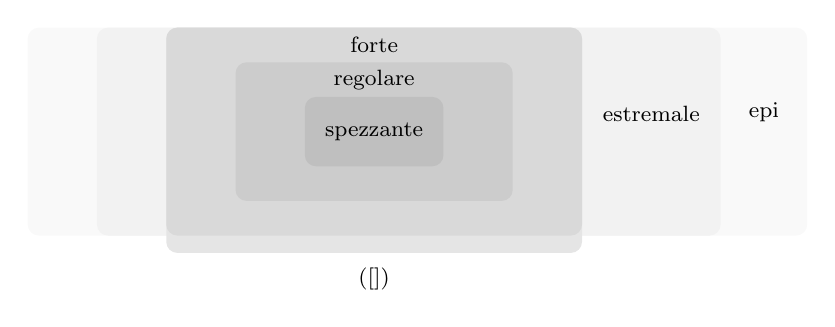
\begin{tikzpicture}[scale=1.1]
   % Outer to inner boxes
   \fill[gray!5,rounded corners] (-4,-1.2) rectangle (5,1.2);
   \node[font=\footnotesize,above] at (4.5,0.0) {epi};

   \fill[gray!10,rounded corners] (-3.2,-1.2) rectangle (4,1.2);
   \node[font=\footnotesize,above] at (3.2,0.0) {estremale};

   \fill[gray!20,rounded corners] (-2.4,-1.4) rectangle (2.4,1.2);
   \node[font=\footnotesize] at (0,-1.7) {$\lort(\Mono[\ctC])$};
   \fill[gray!30,rounded corners] (-2.4,-1.2) rectangle (2.4,1.2);
   \node[font=\footnotesize] at (0,1) {forte};

   \fill[gray!40,rounded corners] (-1.6,-0.8) rectangle (1.6,0.8);
   \node[font=\footnotesize] at (0,0.6) {regolare};

   \fill[gray!50,rounded corners] (-0.8,-0.4) rectangle (0.8,0.4);
   \node[font=\footnotesize] at (0,0) {spezzante};
  \end{tikzpicture}
 \end{center}
 \caption{Gerarchia delle classi di epimorfismi in una categoria \(\ctC\). Le inclusioni si possono invertire sotto le ipotesi indicate. Le classi \(\Epi[\ctC]^s\) degli epi forti di \ref{mepi_forte} e l'ortogonale sinistro \(\lort(\Mono[\ctC])\) sono `essenzialmente sempre' coincidenti nei casi reali, ma \ref{strepi_not_epi} è un controesempio. Ipotesi opportune su \(\ctC\) rovesciano alcune di queste inclusioni.}\label{fig_gerarchia}
\end{figure}
\subsection{Interazioni tra limiti e colimiti, completamenti}\index{Completamento!--- libero}
\subsubsection{Sulla commutatività dei limiti con i colimiti}\label{sec_comm_limcolim}

\begin{color}{blue}
 Questa parte dovrebbe essere la prosecuzione naturale della sezione precedente.
\end{color}

\begin{remark}\label{rem_noncomm_limcolim}
 È importante chiarire che, benché la proposizione \ref{prop_fubini} valga tanto per i limiti che (nella sua versione duale)
 per i colimiti, in generale i limiti non commutano con i colimiti. Precisiamo il problema: se \(G \colon \ctC \times \ctD \fun \ctB\)
 è un funtore, si ha effettivamente una freccia canonica \(\delta\) determinata dalla commutatività del seguente diagramma,
 dove le frecce senza nome sono le frecce canoniche del limite e del colimite
 \[\xymatrix{\colim_{\ctD}(\lim_{\ctC}G(C,D)) \ar[rr]^{\delta} & & \lim_{\ctC}(\colim_{\ctD}G(C,D)) \ar[d] \\
  \lim_{\ctC}G(C,D) \ar[u] \ar[r] & G(C,D) \ar[r] & \colim_{\ctD}G(C,D)}\]
 (ammesso evidentemente che tali limiti e colimiti esistano in \(\ctB\)), ma in generale tale freccia non è un isomorfismo,
 come mostra il seguente esempio.
\end{remark}

\begin{example}\label{ex_noncomm_limcolim}
 Prendiamo \(\ctC = \ctD = \{0,1\}\), la categoria discreta con due oggetti distinti, e \(G \colon \ctC \times \ctD \fun \ctSet\)
 il funtore costante che associa a ogni oggetto l'insieme 2 a due elementi. Il dominio e il codominio della freccia \(\delta\)
 in questo caso sono, rispettivamente, \((2 \times 2) + (2 \times 2)\) e \((2 + 2) \times (2 + 2)\). Per ovvie ragioni di cardinalità,
 non ci può essere nessuna biiezione fra tali insiemi.
\end{example}

Nei teoremi \ref{th_caratt_sifted} e \ref{th_caratt_filtr} espliciteremo due casi importanti in cui la freccia \(\delta\) dell'osservazione
\ref{rem_noncomm_limcolim} è un isomorfismo. Come risultato preliminare alla dimostrazione del teorema \ref{th_caratt_sifted}
ci occorre una caratterizzazione dei funtori iniziali in termini di colimiti. Ci limitiamo a dimostrare solo una delle due implicazioni
(quella che interviene nella prova del teorema), la seconda sarà proposta come esercizio. Ricordiamo che una categoria \(\ctD\) è
connessa se è non vuota e se per ogni coppia di oggetti \(X,Y \in \ctD\) esiste uno zig-zag di frecce che li connette
\[X \longleftarrow D_1 \longrightarrow D_2 \longleftarrow D_3 \longrightarrow D_4 \ldots\ldots D_{n-1} \longleftarrow D_n \longrightarrow Y\]
(vedi esercizio \ref{E.2.6.7}). Ricordiamo anche che un funtore \(F \colon \ctC \fun \ctD\) è iniziale se, per ogni oggetto \(D \in \ctD\), la
categoria comma \(D/F\) è connessa (vedi definizione \ref{2.8.61}).

\begin{lemma}\label{lemma_caract_funt_iniz}
 Un funtore \(F \colon \ctC \fun \ctD\) è iniziale se e solo se per ogni categoria \(\ctA\) e per ogni funtore \(G \colon \ctD \fun \ctA\),
 l'esistenza del colimite di \(G \cdot F\) implica che esiste il colimite di \(G\) e che la freccia canonica
 \[\beta \colon \colim_{\ctC}(G \cdot F) \to \colim_{\ctD}(G)\]
 è un isomorfismo.
\end{lemma}

\begin{proof} Precisiamo che \(\beta\) è l'unica freccia tale che il diagramma
 \[\xymatrix{\colim_{\ctC}(G \cdot F) \ar[rr]^-{\beta} & & \colim_{\ctD}(G) \\
  & G(FC) \ar[lu]^{\sigma_C} \ar[ru]_{s_{FC}} }\]
 commuta per ogni \(C \in \ctC\), dove le frecce \(\sigma_C\) e \(s_D\) sono le iniezioni nel colimite. \\
 \(\Rightarrow \colon\) Dobbiamo costruire il cocono colimite \(\{s_D \colon GD \to \colim_{\ctC}(G \cdot F)\}_{D \in \ctD}\).
 Per un oggetto \(D \in \ctD\) fissato, la categoria comma \(D/F\) è non vuota (perché connessa). Possiamo dunque scegliere
 una freccia \(u_D \colon D \to FX\) e porre
 \[s_D = \sigma_X \cdot G(u_D) \colon GD \to G(FX) \to \colim_{\ctC}(G \cdot F)\]
 Dobbiamo verificare che \(s_D\) è ben definita, cioè non dipende dalla scelta della freccia \(u_D\). Una volta fatto questo,
 la verifica che la famiglia \(\{s_D\}_{D \in \ctD}\) è naturale è simile (ma più semplice) e la verifica della proprietà universale
 è diretta (usando naturalmente la proprietà universale del colimite di \(G \cdot F\)). Supponiamo quindi di avere una seconda
 freccia \(v_D \colon D \to FY\). Poiché \(D/F\) è connessa, si può trovare uno zig-zag in \(D/F\) che connette \(u_D\) e \(v_D\)
 (per semplificare la scrittura dei diagrammi utilizzati nella dimostrazione, supponiamo che lo zig-zag sia ridotto a un'unica spanna,
 ma l'argomento è chiaramente generale), ovvero che si abbia un diagramma commutativo del tipo
 \[\xymatrix{ & D \ar[ld]_{u_D} \ar[d]^{f} \ar[rd]^{v_D} \\
  FX & FZ \ar[l]^-{Fx} \ar[r]_-{Fy} & FY}\]
 Applicando il funtore \(G\) a tale diagramma, si ottiene
 \[\xymatrix{ & &\colim_{\ctC}(G \cdot F) \\
  G(FX) \ar[rru]^{\sigma_X} & & & & GD  \ar[llll]_-{G(u_D)} \ar@{-->}[llu]_{s_D} \ar[llld]_>>>>>>>>>>>>>>>>>>>>{G(f)} \ar[ld]^{G(v_D)} \\
  & G(FZ) \ar[lu]^{G(Fx)} \ar[ruu]^>>>>>>>>>>{\sigma_Z} \ar[rr]_{G(Fy)} & & G(FY) \ar[luu]_>>>>>>>>>>{\sigma_Y} }\]
 Bisogna mostrare che \(\sigma_X \cdot G(u_D) = \sigma_Y \cdot G(v_D)\) usando la naturalità del cocono \(\{\sigma_C\}_{C \in \ctC} \colon\)
 \[\sigma_X \cdot G(u_D) = \sigma_X \cdot G(Fx) \cdot G(f) = \sigma_Z \cdot G(f) = \sigma_Y \cdot G(Fy) \cdot G(f) = \sigma_Y \cdot G(v_D)\]
 Consideriamo che questo sia sufficiente come dimostrazione della prima implicazione.
\end{proof}

Per la prova del teorema \ref{th_caratt_sifted} ci saranno utili 	anche i seguenti facili esercizi.

\begin{exercise}\label{exer_set_conn}
 Ogni categoria setacciata è connessa.
\end{exercise}

\begin{exercise}\label{exer_colim_cost}
 Sia \(F \colon \ctD \fun \ctB\) un funtore costante di valore \(X \in \ctB\). Se \(\ctD\) è connessa, allora il colimite di \(F\)
 è \(\{\id_X \colon F(D) = X \to X\}_{D \in \ctD}\). (Se \(X\) è l'oggetto iniziale di \(\ctB\), allora l'ipotesi che \(\ctD\) sia
 connessa è superflua.)
\end{exercise}

Enunciamo ora i due teoremi che caratterizzano le categorie setacciate e filtrate in termini di commutazione fra limiti e colimiti.
Per il momento ci limitiamo a dimostrare l'implicazione \(\Rightarrow\) del teorema \ref{th_caratt_sifted}, in quanto è quella
che serve nel capitolo \ref{cap_cat_alg}, dedicato alle categorie algebriche, per costruire certi colimiti. L'implicazione opposta e
la dimostrazione del teorema \ref{th_caratt_filtr} saranno proposte come esercizi.

\begin{theorem}\label{th_caratt_sifted}
 Una categoria piccola \(\ctD\) è setacciata (nel senso della definizione \ref{2.5.44}) se e solo se per ogni categoria discreta e
 finita \(\ctC\) e per ogni funtore \(G \colon \ctC \times \ctD \fun \ctSet\), la freccia canonica
 \[\delta \colon \colim_{\ctD}(\lim_{\ctC}G(C,D)) \to \lim_{\ctC}(\colim_{\ctD}G(C,D))\]
 è un isomorfismo.
\end{theorem}

\begin{proof} \(\Rightarrow \colon\) Assumiamo che la categoria \(\ctD\) sia setacciata e mostriamo che la freccia \(\delta\)
 dell'osservazione \ref{rem_noncomm_limcolim} è un isomorfismo. Poiché \(\ctC\) è finita e discreta, per induzione
 basta considerare due casi, il caso in  cui \(\ctC\) contiene solo due elementi distinti e il caso in  cui \(\ctC\) è vuota. \\
 Caso \(\ctC = \{1,2\} \colon\) in questa situazione dare un funtore \(G \colon \ctC \times \ctD \fun \ctSet\) significa scegliere due
 funtori \(H_1 = G(1,-), H_2 = G(2,-) \colon \ctD \fun \ctSet\). La freccia \(\delta\) è dunque
 \[\xymatrix{\colim_{\ctD}(H_1 \times H_2) \ar[rr]^-{\delta} & & \colim_{\ctD}(H_1) \times \colim_{\ctD}(H_2) \\
  & H_1(D) \times H_2(D) \ar[lu]^{\sigma_D} \ar[ru]_{s^1_D \times s^2_D} }\]
 dove \(H_1 \times H_2 \colon \ctD \fun \ctSet\) è il prodotto di \(H_1\) e \(H_2\) nella categoria \(\ctSet^{\ctD}\) (vedi proposizione
 \ref{prop_lim_puntuali}) e \(\{\sigma_D\}_{D \in \ctD}, \{s^1_D\}_{D \in \ctD}, \{s^2_D\}_{D \in \ctD}\) sono i coconi colimite.
 Osserviamo che
 \[\xymatrix{ & \ctD \times \ctD \ar[rd]^{H_1 \boxtimes H_2} \\
   \ctD \ar[ru]^{\Delta} \ar[rr]_{H_1 \times H_2} & & \ctSet }\]
 dove \(\Delta(D) = (D,D)\) e \(H_1 \boxtimes H_2)(D_1,D_2) = H_1(D_1) \times H_2(D_2)\) (questo è un caso particolarmente
 semplice dell'esercizio \ref{exer_lim_puntuali}). Poichè \(\ctD\) è setacciata, il funtore \(\Delta\) è iniziale (teorema \ref{2.8.65})
 e quindi, per il lemma \ref{lemma_caract_funt_iniz}, si ha un isomorfismo
 \[\beta \colon \colim_{\ctD}(H_1 \times H_2) = \colim_{\ctD}((H_1 \boxtimes H_2) \cdot \Delta) \to
  \colim_{\ctD \times \ctD}(H_1 \boxtimes H_2)\]
 Per mostrare che \(\delta = \beta\), e quindi che \(\delta\) è un isomorfismo, rimane da provare che
 \[\{s^1_{D_1} \times s^2_{D_2} \colon H_1(D_1) \times H_2(D_2) \to
  \colim_{\ctD}(H_1) \times \colim_{\ctD}(H_2)\}_{(D_1,D_2) \in \ctD \times \ctD}\]
 è il cocono colimite del funtore \(H_1 \boxtimes H_2\). Questa è una conseguenza del fatto che \(\ctSet\) è cartesiana chiusa
 (esempio \ref{ex_set_cartcl}). Esplicitamente, dato un cocono
 \[\{x_{D_1,D_2} \colon H_1(D_1) \times H_2(D_2) \to X\}_{(D_1,D_2) \in \ctD \times \ctD}\]
 l'unica fattorizzazione \(x \colon \colim_{\ctD}(H_1) \times \colim_{\ctD}(H_2) \to X\) delle frecce \(x_{D_1,D_2}\) attraverso le frecce
 \(s^1_{D_1} \times s^2_{D_2}\) si ottiene grazie alle seguenti biiezioni naturali fra l'insieme delle funzioni al di sopra della linea
 orizzontale e l'insieme delle funzioni al di sotto della linea:
 \[\begin{array}{c}
   x \colon \colim_{\ctD}(H_1) \times \colim_{\ctD}(H_2) \to X           \\ \hline
   \colim_{\ctD}(H_2) \to \ctSet(\colim_{\ctD}(H_1),X)                   \\ \hline
   \{H_2(D_2) \to \ctSet(\colim_{\ctD}(H_1),X)\}_{D_2 \in \ctD}          \\ \hline
   \{\colim_{\ctD}(H_1) \times H_2(D_2) \to X\}_{D_2 \in \ctD}           \\ \hline
   \{\colim_{\ctD}(H_1) \to \ctSet(H_2(D_2),X)\}_{D_2 \in \ctD}          \\ \hline
   \{\{H_1(D_1) \to \ctSet(H_2(D_2),X)\}_{D_1 \in \ctD}\}_{D_2 \in \ctD} \\ \hline
   \{\{x_{D_1,D_2} \colon H_1(D_1) \times H_2(D_2) \to X\}_{D_1 \in \ctD}\}_{D_2 \in \ctD}
  \end{array}\]
 Caso \(\ctC = \emptyset \colon\) in questa situazione la freccia \(\delta\) è la freccia terminale
 \[\delta \colon \colim_{\ctD}(T) \to \{\ast\}\]
 dove \(T \colon \ctD \fun \ctSet\) è l'oggetto terminale della categoria \(\ctSet^{\ctD}\), cioè il funtore costante definito
 da \(T(D) = \{\ast\}\). Poichè \(\ctD\) è setacciata, è anche connessa (esercizio \ref{exer_set_conn}) e quindi l'esercizio
 \ref{exer_colim_cost} permette di concludere che \(\delta\) è un isomorfismo.
\end{proof}

\begin{theorem}\label{th_caratt_filtr}
 Una categoria piccola \(\ctD\) è filtrata (nel senso della definizione \ref{2.5.41}) se e solo se per ogni categoria
 finite \(\ctC\) e per ogni funtore \(G \colon \ctC \times \ctD \fun \ctSet\), la freccia canonica
 \[\delta \colon \colim_{\ctD}(\lim_{\ctC}G(C,D)) \to \lim_{\ctC}(\colim_{\ctD}G(C,D))\]
 è un isomorfismo.
\end{theorem}

\begin{remark}\label{oss_unioni_filtr_sg}
 Per aiutare la lettrice a capire l'interesse dei teoremi \ref{th_caratt_sifted} e \ref{th_caratt_filtr} ricordiamo che, come già detto,
 nel capitolo \ref{cap_cat_alg} essi saranno utilizzati per mostrare che nelle categorie algebriche i colimiti setacciati si calcolano
 come colimiti degli insiemi soggiacenti (in un senso che verrà precisato), come è per altro il caso di tutti i limiti nelle categorie
 algebriche. Per vedere un esempio facile di tale situazione, si può pensare a una famiglia \(\{H_i\}_{i \in I}\) di sottogruppi di un
 gruppo \(G\), famiglia indicizzata da un insieme \(I\). L'intersezione insiemistica \(\bigcap_{i \in I}H_i\)  (che è un tipo di limite)
 è chiaramente un sottogruppo di \(G\). Invece l'unione \(\bigcup_{i \in I}H_i\) (che è un colimite) in generale non lo è.
 Se però l'insieme \(I\) è un insieme ordinato in cui ogni sottoinsieme finito ammette un maggiorante (e in particolare se è un
 insieme totalmente ordinato), ovvero se, visto come categoria, è filtrata, allora l'unione (che diventa in tal caso un colimite filtrato)
 è chiaramente un sottogruppo. Questa situazione, benché semplice, è di notevole importanza: si pensi alla dimostrazione
 del teorema di Krull (ogni ideale proprio di un anello commutativo è contenuto in un ideale massimale) o al fatto che in un
 anello noetheriano ogni catena ascendente di ideali si stabilizza.
\end{remark}


\begin{proposition}[Commutatività di colimiti filtrati e limiti finiti]\label{prop_commutativita_colimiti_filtrati_limiti_finiti}\index{Colimite!filtrato!commutatività con limiti finiti}\index{Limite!finito!commutatività con colimiti filtrati}
 \Todo{}
\end{proposition}

\begin{proposition}[Commutatività di colimiti setacciati e prodotti]\label{prop_commutativita_colimiti_setacciati_prodotti}\index{Colimite!--- setacciato}
 \Todo{}
\end{proposition}

\begin{definition}[Categoria di funtori polinomiali]\label{def_categoria_funtori_polinomiali}\index{Funtore!polinomiale}\index{Funtore!--- polinomiale}
 limiti e colimiti interagiscono per formare un polinomio
 \Todo{}
\end{definition}
\begin{example}\label{ex_colim_liste}\index{Liste!--- come colimite}
 \Todo{Liste come polinomi}
\end{example}
\begin{definition}[Completamento libero per diagrammi di forma \(\ctJ\)]\label{def_completamento_libero_diagrammi_ctJ}
 \Todo{}
\end{definition}

\Todo{Questa parte va riordinata secondo uno schema più razionale oppure rischia di diventare lunghissima e dispersiva; i completamenti liberi sono importanti, quindi vorrei dare: la definizione generale, l'esempio del completamento per coprodotti (e dualmente allora per prodotti) e il completamento di Cauchy; quindi copio `brutalmente' quello che ha scritto EnricoV e lo metteremo a posto}
\subsubsection{Completamento libero per prodotti}\label{sec_compl_somme_e_prod}
\Todo{}
\subsubsection{Completamento libero per idempotenti}\label{sec_compl_idemp}

\begin{color}{blue}
 Il completamento per idempotenti di una categoria è un argomento interessante che rientra nei teoremi di dualità
 per le teorie algebriche. Non so bene quale è il punto migliore del libro per introdurlo. Porta vari nomi: completamento per
 idempotenti, Cauchy completion, Karoubi envelope, \ldots Esito fra completamento per idempotenti e il più suggestivo
 completamento di Cauchy, che però, se adottato, richiede una spiegazione.
\end{color}

\hfill

Come secondo esempio di completamento, studiamo il completamento per idempotenti di una categoria.

\begin{definition}\label{def_idempotente}
 Una freccia \(f \colon X \to X\) di una categoria è detta idempotente se \(f \cmp f = f\).
\end{definition}

\begin{remark}\label{oss_idemp_eq}
 Dalla proposizione \ref{prop_equal_ass} sappiamo che, a partire da un diagramma commutativo del tipo
 seguente (che esprime il fatto che \(R\) è un  retratto di \(X\))
 \[ \xymatrix{R \ar[rr]^-{\id_R} \ar[rd]_{s} & & R \\ & X \ar[ru]_{r} } \]
 si ottengono un equalizzatore assoluto e un coequalizzatore assoluto nel modo seguente
 \[\xymatrix{R \ar[r]^-{s} & X \ar@<0.5ex>[r]^-{s \cmp r} \ar@<-0.5ex>[r]_-{\id_X} & X}
  \;\;\;\;\;\;\;\;\;\;\;\;
  \xymatrix{X \ar@<0.5ex>[r]^-{s \cmp r} \ar@<-0.5ex>[r]_-{\id_X} & X \ar[r]^-{r} & R}\]
 Osserviamo che la freccia \(s \cmp r \colon X \to X\) è idempootente, infatti \(s \cmp r \cmp s \cmp r = s \cmp \id \cmp r = s \cmp r\). \\
 Il prossimo lemma chiarisce il legame fra l'idempotenza della freccia \(s \cmp r\) e l'esistenza dell'equalizzatore e del coequalizzatore
 della coppia \((s \cmp r, \id_X)\).
\end{remark}

\begin{lemma}\label{lemma_spezz_idemp}
 Sia \(f \colon X \to X\) una freccia in una categoria \(\ctA\). Le condizioni seguenti sono equivalenti:
 \begin{enumerate}
  \item La freccia \(f\) si spezza: esistono \(s \colon R \to X\) ed \(r \colon X \to R\) tali che \(s \cmp r = f\) ed
        \(r \cmp s = \id_R\).
  \item La freccia \(f\) è idempotente ed esiste l'equalizzatore \(\xymatrix{R \ar[r]^-{s} & X \ar@<0.5ex>[r]^-{f} \ar@<-0.5ex>[r]_-{\id_X} & X}\)
  \item La freccia \(f\) è idempotente ed esiste il coequalizzatore \(\xymatrix{X \ar@<0.5ex>[r]^-{f} \ar@<-0.5ex>[r]_-{\id_X} & X \ar[r]^-{r} & R}\)
 \end{enumerate}
\end{lemma}

\begin{proof}
 \(1 \Rightarrow 2\) e \(1 \Rightarrow 3 \colon\) Questo è il contenuto della proposizione \ref{prop_equal_ass} e
 dell'osservazione \ref{oss_idemp_eq}. \\
 Ora mostriamo che \(2 \Rightarrow 1\), la prova dell'implicazione \(3 \Rightarrow 1\) è duale. Poiché \(f\) è
 idempotente, si ha \(f \cmp f = f = \id_X \cmp f\). La propriet\'a universale dell'equalizzatore fornisce un'unica freccia
 \(s \colon X \to R\) tale che \(s \cmp r = f\). Resta da mostrare che \(r \cmp s = \id_R\). Poiché \(s\) è un mono, tale
 uguaglianza si deduce dal fatto che \(s\) equalizza \(f\) e \(\id_X\), infatti \(s \cmp r \cmp s = f \cmp s = \id_X \cmp s = s \cmp \id_R\).
\end{proof}

\begin{definition}\label{def_idemp_compl}
 Una categoria è completa per idempotenti se tutte le sue frecce idempotenti si spezzano.
\end{definition}

\begin{remark}\label{oss_idCompl_retr}
 Segnaliamo qualche semplice conseguenza del lemma \ref{lemma_spezz_idemp}:
 \begin{enumerate}
  \item Una categoria che ha gli equalizzatori (o i coequalizzatori), è completa per idempotenti.
  \item Il fatto di essere completa per idempotenti è una condizione autoduale: una categoria \(\ctC\)
        è completa per idempotenti se e solo se \(\ctC^{\op}\) lo è.
  \item Una sottocategoria piena \(\ctB\) di una categoria \(\ctA\) completa per idempotenti è a sua
        volta completa per idempotenti se e solo se è chiusa in \(\ctA\) per retratti.
  \item Lo spezzamento di una freccia idempotente, quando esiste, è unico a meno di isomorfismi.
 \end{enumerate}
\end{remark}

Vediamo come si può costruire in modo universale una categoria completa per idemopotenti a partire da una categoria qualsiasi.

\begin{proposition}\label{prop_compl_idemp}
 Sia \(\ctC\) una categoria. Esistono una categoria completa per idempotenti \(\mathrm{Ic}(\ctC)\) e un funtore
 \(\mathrm{Ic}_{\ctC} \colon \ctC \fun \mathrm{Ic}(\ctC)\) tali che, per ogni categoria completa per idempotenti \(\ctB\) e per
 ogni funtore \(F \colon \ctC \fun \ctB\), esiste un funtore \(F' \colon \mathrm{Ic}(\ctC) \fun \ctB\) tale che il diagramma
 \[ \xymatrix{\ctC \ar[rr]^-{\mathrm{Ic}_{\ctC}} \ar[rd]_{F} & & \mathrm{Ic}(\ctC) \ar[ld]^{F'} \\ & \ctB }\]
 commuta a meno di un isomorfismo naturale. Inoltre, tale funtore \(F'\) è essenzialmente unico.
\end{proposition}

\begin{proof}
 Cominciamo col descrivere la categoria \(\mathrm{Ic}(\ctC)\).Un oggetto de \(\mathrm{Ic}(\ctC)\) è una freccia idempotente
 \(f \colon X \to X\) di \(\ctC\). Una freccia \(a \colon (f \colon X \to X) \to (g \colon Y \to Y)\) è una freccia \(a \colon X \to Y\) di
 \(\ctC\) tale che \(g \cmp a \cmp f = a\) o, equivalentemente, tale che \(a \cmp f = a\) e \(g \cmp a = a\)
 \[ \xymatrix{X \ar[r]^-{a} \ar[d]_{f} & Y \ar[d]^{g} \\
  X \ar[ru]^{a} \ar[r]_-{a} & Y }\]
 In effetti, se \(a \cmp f = f\) e \(g \cmp a = a\), allora \(g \cmp a \cmp f = g \cmp a = a\); viceversa, se \(g \cmp a \cmp f = a\),
 allora \(g \cmp a = g \cmp g \cmp a \cmp f = g \cmp a \cmp f = a\) e, analogamente, \(a \cmp f = a\). La composizione in
 \(\mathrm{Ic}(\ctC)\) è quella di \(\ctC\). La freccia identità in \(\mathrm{Ic}(\ctC)\) è
 \(f \colon (f \colon X \to X) \to (f \colon X \to X)\).
 Il funtore \(\mathrm{Ic}_{\ctC} \colon \ctC \fun \mathrm{Ic}(\ctC)\) è definito da
 \[ a \colon X \to Y \;\mapsto \; a \colon (\id_X \colon X \to X) \to (\id_Y \colon Y \to Y)\]
 Se \(h \colon (f \colon X \to X) \to (f \colon X \to X)\) è una freccia idempotente in \(\mathrm{Ic}(\ctC)\), il suo spezzamento è
 \[ (f \colon X \to X) \xto{h} (h \colon X \to X) \xto{h} (f \colon X \to X) \]
 Questo dimostra che \(\mathrm{Ic}(\ctC)\) è completa per idempotenti. \\
 Verifichiamo ora la proprietà universale. Se si applica la descrizione dello spezzamento di
 una freccia idempotente al caso dell'immagine in \(\mathrm{Ic}(\ctC)\) di una freccia idempotente \(f \colon X \to X\) di \(\ctC\),
 ne segue che, per ogni freccia \(a \colon (f \colon X \to X) \to (g \colon Y \to Y)\) di \(\mathrm{Ic}(\ctC)\), le due righe del
 diagramma commutativo
 \[ \xymatrix{(X \xto{f} X) \ar[rr]^-{f} \ar[d]_{a} & &
  \mathrm{Ic}_{\ctC}(X) \ar@<0.5ex>[rr]^-{\mathrm{Ic}_{\ctC}(f)} \ar@<-0.5ex>[rr]_-{\id} \ar[d]_{\mathrm{Ic}_{\ctC}(a)}
  & & \mathrm{Ic}_{\ctC}(X) \ar[d]^{\mathrm{Ic}_{\ctC}(a)} \\
  (Y \xto{g} Y) \ar[rr]_-{g} & & \mathrm{Ic}_{\ctC}(Y) \ar@<0.5ex>[rr]^-{\mathrm{Ic}_{\ctC}(g)} \ar@<-0.5ex>[rr]_-{\id}
  & & \mathrm{Ic}_{\ctC}(Y) }\]
 sono equalizzatori assoluti. Se ora abbiamo un funtore \(F \colon \ctC \fun \ctB\), l'unico modo di definire un funtore
 \(F' \colon \mathrm{Ic}(\ctC) \fun \ctB\) tale che \(F' \cmp \mathrm{Ic}_{\ctC} \simeq F\) è di definirlo come l'estensione
 agli equalizzatori nel diagramma seguente
 \[ \xymatrix{F'(f) \ar[r] \ar[d]_{F'(a)} & FX \ar@<0.5ex>[rr]^-{F(f)} \ar@<-0.5ex>[rr]_-{\id} \ar[d]_{F(a)} & & FX \ar[d]^{F(a)} \\
  F'(g) \ar[r] & FY \ar@<0.5ex>[rr]^-{F(g)} \ar@<-0.5ex>[rr]_-{\id} & & FY }\]
 Tale definizione è possibile perché \(\ctB\) è completa per idempotenti e le frecce \(F(f)\) e \(F(g)\) sono idempotenti.
\end{proof}

Per esprimere la proprietà universale \ref{prop_compl_idemp} in termini di un'equivalenza di categorie, utilizziamo un
lemma generale che richiede la nozione di suriettività a meno di retratti.

\begin{definition}\label{fef_sur_utr}
 Un funtore \(M \colon \ctC \fun \ctD\) è suriettivo a meno di retratti se ogni oggetto di \(\ctD\) è un retratto di un pggetto
 proveniente da \(\ctC\): per ogni \(D \in \ctD\) esiste un oggetto \(X \in \ctC\) e un diagramma del tipo
 \[\xymatrix{D \ar[rr]^-{\id_D} \ar[rd]_{s} & & D \\ & MX \ar[ru]_{r} }\]
\end{definition}

\begin{lemma}\label{lemma_indsur}
 Siano \(\ctB\) una categoria ed \(M\colon \ctC \fun \ctD\) un funtore. Consideriamo il funtore \(\ctB^M \colon \ctB^\ctD \fun \ctB^\ctC\)
 indotto per composizione con \(M\).
 \begin{enumerate}
  \item Se \(M\) è suriettivo a meno di retratti, allora \(\ctB^M\) è fedele.
  \item Se \(M\) è pieno e suriettivo a meno di retratti, allora \(\ctB^M\) è pieno e fedele.
 \end{enumerate}
\end{lemma}

\begin{proof}
 1. Consideriamo due trasformazioni naturali \(\beta,\gamma \colon A \nat B \colon \ctD \rightrightarrows \ctB\) e supponiamo
 che per ogni oggetto \(X \in \ctC\) si abbia \(\beta_{MX} = \gamma_{MX} \colon AMX \to BMX\). Per un oggetto \(D \in \ctD\),
 scegliamo una presentazione del tipo
 \[(X \in \ctC, s \colon D \to MX, r \colon MX \to D, r \cmp s = \id_D)\]
 La commutatività del diagramma seguente, dovuta alla naturalità di \(\beta\) e \(\gamma\), mostra che
 \(\beta_D = \gamma_D\), il che conclude la prova della fedeltà del funtore \(\ctB^M\)
 \[\xymatrix{AD \ar[r]^-{As} \ar[d]_{\beta_D} & AMX \ar[r]^-{Ar} \ar[d]_{\beta_{MX}} \ar[d]|{=} \ar[d]^{\gamma_{MX}} & AD \ar[d]^{\gamma_D} \\
  BD \ar[r]_-{Bs} & BMX \ar[r]_-{Br} & BD }\]
 2. Sia ora \(\alpha \colon A \cmp M \nat B \cdot M \colon \ctC \rightrightarrows \ctB\) una trasformazione naturale. Cerchiamo
 una trasformazione naturale \(\beta \colon A \nat B \colon \ctD \rightrightarrows \ctB\) tale che \(\ctB^M(\beta) = \alpha\).
 Per un oggetto \(D \in \ctD\), scegliamo una presentazione
 \[(X \in \ctC, s \colon D \to MX, r \colon MX \to D, r \cmp s = \id_D)\]
 e poniamo
 \[\beta_D \colon \xymatrix{AD \ar[r]^-{As} & AMX \ar[r]^-{\alpha_X} & BMX \ar[r]^-{Br} & BD}\]
 Cominciamo col mostrare il carattere naturale della famiglia \(\beta = \{\beta_D \colon AD \to BD \mid D \in \ctD\}\). Per questo, sia
 \(h \colon D \to E\) una freccia in \(\ctD\) e scegliamo una presentazione
 \[(Y \in \ctC, v \colon E \to MY, u \colon MY \to E, u \cmp v = \id_E)\]
 per l'oggetto \(E\). Otteniamo una freccia \(v \cmp h \cmp r \colon MX \to MY\) e, poiché \(M\) è pieno, esiste una freccia
 \(f \colon X \to Y\) tale che \(M(f) = v \cmp h \cmp r\). Ora possiamo considerare il diagramma seguente, la cui commutatività mostra
 il carattere naturale di \(\beta\):
 \[\xymatrix{AD \ar[r]^-{As} \ar[d]_{Ah} & AMX \ar[r]^-{\alpha_X} \ar[d]_{AMf} & BMX \ar[r]^-{Br} \ar[d]^{BMf} & BD \ar[d]^{Bh} \\
  AE \ar[r]_-{Av} & AMY \ar[r]_-{\alpha_Y} & BMY \ar[r]_-{Bu} & BE }\]
 Il quadrato centrale commuta per la naturalità di \(\alpha\), il quadrato a destra commuta perché \(u
 \cmp M(f) = u \cmp v \cmp h \cmp r = h \cmp r\) e il quadrato di sinistra commuta perché \(M(f) \cmp s = v \cmp h \cmp r \cmp s = v \cmp h\).
 Se ora scegliamo \(E=D\) e \(h=\id_D\), lo stesso argomento mostra che \(\beta\) è ben definiuta, cioè \(\beta_D\) non dipende
 dalla presentazione scelta per \(D\). In particolrae, se \(D=MX\), come prsentazione possiamo scegliere
 \[(X \in \ctC, \id_{MX} \colon MX \to MX, \id_{MX} \colon MX \to MX)\]
 e otteniamo che \(\beta_{MX} = \alpha_X\), cioè che \(\ctB^M(\beta)=\alpha\).
\end{proof}

\begin{corollary}\label{cor_equiv_idcompl}
 Consideriamo due categorie \(\ctB\) e \(\ctC\), con \(\ctB\) completa per idempotenti. Il funtore
 \(\mathrm{Ic}_\ctC \colon \ctC \fun \mathrm{Ic}(\ctC)\) induce un'equivalenza
 \(\ctB^{\mathrm{Ic}_{\ctC}} \colon \ctB^{\mathrm{Ic}(\ctC)} \fun \ctB^\ctC\).
\end{corollary}

\begin{proof}
 Il funtore \(\mathrm{Ic}_{\ctC}\) è chiaramente pieno. Inoltre è anche suriettivo a meno di retratti perché il diagramma
 \[ \xymatrix{ (X \xto{f} X) \ar[r]^-{f} & \mathrm{Ic}_{\ctC}(X) \ar[r]^-{f} & (X \xto{f} X) }\]
 mostra che ogni oggetto di \(\mathrm{Ic}(\ctC)\) è un retratto di un oggetto proveniente da \(\ctC\). Qunidi il lemma
 \ref{lemma_indsur} garantisce che \(\ctB^{\mathrm{Ic}_{\ctC}}\) è pieno e fedele. Il carattere essenzialmente suriettivo di
 \(\ctB^{\mathrm{Ic}_{\ctC}}\) segue immediatamente dalla proprietà universale \ref{prop_compl_idemp}.
\end{proof}

Nel caso in cui la categoria \(\ctC\) sia piccola, ci tornerà utile più tardi una descrizione alternativa del completamento
per idempotenti (corollario \ref{cor_idcompl_ap}). Per preparare tale descrizione, e per completare il corollario
\ref{cor_equiv_idcompl}, analizziamo la proprietà universale di \(\mathrm{Ic}_{\ctC} \colon \ctC \fun \mathrm{Ic}(\ctC)\).

\begin{lemma}\label{lemma_caratt_idcompl}
 Siano \(\ctC\) e \(\ctD\) due categorie, con \(\ctD\) completa per idempotenti.
 Consideriamo la situazione della proposizione \ref{prop_compl_idemp}
 \[ \xymatrix{\ctC \ar[rr]^-{\mathrm{Ic}_{\ctC}} \ar[rd]_{M} & & \mathrm{Ic}(\ctC) \ar[ld]^{M'} \\ & \ctD }\]
 \begin{enumerate}
  \item Il funtore \(M'\) è un'equivalenza se e solo se \(M\) è pieno, fedele e suriettivo a meno di retratti.
  \item In particolare, \(\ctC\) è completa per idempotenti se e solo se \(\mathrm{Ic}_{\ctC}\) è un'equivalenza.
 \end{enumerate}
\end{lemma}

\begin{proof}
 1. Il funtore \(\mathrm{Ic}_{\ctC}\) è pieno, fedele e suriettivo a meno di retratti, come spiegato nella dimostrazione
 del corollario  \ref{cor_equiv_idcompl}. \\
 Viceversa, le frecce \((f \colon X \to X) \to (g \colon Y \to Y)\) di \(\mathrm{Ic}(\ctC)\) si riconducono a frecce del tipo
 \((f \colon X \to X) \to \mathrm{Ic}_{\ctC}(Y)\) perché \((g \colon Y \to Y)\) è un limite di oggetti provenienti da \(\ctC\). Inoltre,
 le frecce del tipo \((f \colon X \to X) \to \mathrm{Ic}_{\ctC}(Y)\) si riconducono a loro volta a frecce del tipo
 \(\mathrm{Ic}_{\ctC}(X) \to \mathrm{Ic}_{\ctC}(Y)\) perché \((f \colon X \to X)\) è un colimite di oggetti provenienti da \(\ctC\).
 Ma l'azione di \(M'\) su una freccia del tipo \(\mathrm{Ic}_{\ctC}(X) \to \mathrm{Ic}_{\ctC}(Y)\) coincide con l'azione di \(M\)
 sulla corrispondente freccia \(X \to Y\) e quindi \(M'\) è pieno e fedele se \(M\) lo è. Sia ora \(D \in \ctD\). Per ipotesi,
 esistono un oggetto \(X \in \ctC\) e due frecce \(s \colon D \to MX\) e \(r \colon MX \to D\) tali che \(r \cmp s = \id_D\). Poiché
 \(M\) è pieno, esiste una freccia \(f \colon X \to X\) tale che \(M(f) = s \cmp r\). Inoltre, tale freccia \(f\) è idempotente perché
 \(M(f)\) lo è e \(M\) è fedele. Finalmente, \(M'(f)\) è per definizione lo spezzamento di \(M(f)\) in \(\ctD\) e quindi è isomorfo
 a \(D\) perché lo spezzamento è essenzialmente unico. \\
 2. Se \(\mathrm{Ic}_{\ctC}\) è un'equivalenza, allora \(\ctC\) è completa per idempotenti perché \(\mathrm{Ic}(\ctC)\) lo è.
 Viceversa, se \(\ctC\) è completa per idempotenti, si può applicare il punto precedente prendendo come funtore \(F\) il funtore
 identico su \(\ctC\) e si ottiene che \(\mathrm{Ic}_{\ctC}\) è un'equivalenza.
\end{proof}

\begin{corollary}\label{cor_equiv_sutr}
 Consideriamo tre categorie \(\ctB, \ctC\) e \(\ctD\), con \(\ctB\) e \(\ctD\) complete per idempotenti, e un funtore \(M \colon \ctC \fun \ctD\).
 Se \(M\) è pieno, fedele e suriettivo a meno di retratti, allora il funtore indotto \(\ctB^M \colon \ctB^\ctD \fun \ctB^\ctC\) è
 un'equivalenza.
\end{corollary}

\begin{proof}
 Dalla decomposizione \(M = M' \cmp \mathrm{Ic}_\ctC\) della proposizione \ref{prop_compl_idemp} segue che
 \(\ctB^M = \ctB^{M' \cmp \mathrm{Ic}_{\ctC}} = \ctB^{\mathrm{Ic}_{\ctC}} \cmp \ctB^{M'}\). Poiché \(\ctB^{\mathrm{Ic}_{\ctC}}\)
 è un'equivalenza (corollario \ref{cor_equiv_idcompl}) e \(\ctB^{M'}\) è un'equivalenza (lemma \ref{lemma_caratt_idcompl}),
 anche \(\ctB^M\) è un'equivalenza.
\end{proof}

\begin{remark}\label{oss_idcompl_duale}
 Poiché il fatto di essere completa per idempotenti è una condizione autoduale, possiamo applicare il lemma
 \ref{lemma_caratt_idcompl} alla configurazione
 \[ \xymatrix{\ctC^{\op} \ar[rr]^-{\mathrm{Ic}_{\ctC^{\op}}} \ar[rd]_{M=\mathrm{Ic}_{\ctC}^{\op}} & & \mathrm{Ic}(\ctC^{\op}) \ar[ld]^{M'} \\
  & \mathrm{Ic}(\ctC)^{\op} }\]
 e il funtore \(M'\) che si ottiene fornisce un'equvalenza \(\mathrm{Ic}(\ctC^{\op}) \simeq \mathrm{Ic}(\ctC)^{\op}\).
\end{remark}

\begin{theorem}[Complemento]\label{mk_kelly_closure}
 Kelly closure of a class of colimits
 \cite{paper_kelly_closure}
 \Todo{}
\end{theorem}

% \input{cap/02/sec/05-costruzioni-con-limiti.tex}
\section{Limiti e colimiti nella pratica matematica}
perché si chiamano limiti?
\begin{remark}
 \Todo{Limiti in analisi come limiti categoriali}
\end{remark}
\subsection{Limiti in algebra, topologia e logica}
\begin{example}\label{ex_lim_kernel}
 Il \emph{nucleo} di una applicazione lineare \(f \colon V \to W\) tra spazi vettoriali (o tra gruppi abeliani, o \(R\)-moduli,\dots), già introdotto in \ref{ker_e_coker}, è un esempio di limite: si tratta dell'equalizzatore della coppia
 % https://q.uiver.app/#q=WzAsMixbMCwwLCJWIl0sWzEsMCwiVyJdLFswLDEsIjAiLDAseyJvZmZzZXQiOi0yfV0sWzAsMSwiZiIsMix7Im9mZnNldCI6MX1dXQ==
 \[\begin{tikzcd}[cramped]
   V & W
   \arrow["0", shift left=2, from=1-1, to=1-2]
   \arrow["f"', shift right, from=1-1, to=1-2]
  \end{tikzcd}\]
 In effetti una nozione di `nucleo' in questo senso si può dare in ogni categoria che abbia un \emph{oggetto zero}, nel senso di un oggetto che sia allo stesso tempo iniziale e terminale (questo è il caso di ciascuna delle categorie appena menzionate, ma anche della categoria degli insiemi puntati di \ref{}). In tal caso, si ricordi che la `mappa zero' consiste della composizione \(0_{VW} \colon V \to 0 \to W\) e in un certo senso evidente \(\ker f\) è in quel caso il massimo sottoggetto \(i_{\ker f} \colon \ker f \mono V\) tale che \(f\circ i_{\ker f} = 0_{VW}\). Nel caso degli insiemi puntati, dove \(V=(A,a_0)\), si tratta del sottoinsieme \(K\subseteq A\) determinato come \(K=\{a\in A\mid fa = b_0\}\), se \(W=(B,b_0)\) è l'insieme puntato codominio.
\end{example}
\begin{example}\label{exa_sottoggetti_limite}\index{Funtore!--- dei sottoggetti}\index{Sottoggetto}
 Il funtore dei sottoggetti introdotto in \ref{def_fun_sub_onset} fa uso della nozione di prodotto fibrato in \(\ctSet\): infatti, data una funzione \(u \colon A\to B\) tra insiemi, la funzione \(\Sub(u) \colon \Sub(B) \to \Sub(A)\) si determina dal prodotto fibrato
 \[\begin{tikzcd}
   u^*E =\pull AEB \arrow[r] \arrow[d, hook] & E \arrow[d, hook] \\
   A \arrow[r, "u"'] & B
  \end{tikzcd}\]
 Infatti, la funzione \(\Sub(u)\) manda un sottoggetto \(E\mono B\) nel sottoggetto \(u^*E\mono A\).
\end{example}

\begin{example}\label{exa_grafico_limite}\index{Grafico!--- di una funzione}
 \Todo{Grafici di funzioni}
\end{example}

\begin{example}\label{exa_tabulatore_relazione_limite}\index{Tabulatore}\index{Relazione}
 \Todo{Tabulatore di una relazione}
\end{example}

\begin{example}\label{exa_punti_fissi_limite}\index{Punto fisso}\index{Limite!Punti fissi come ---e}
 \Todo{Punti fissi come limiti}
\end{example}

\begin{example}\label{exa_categoria_elementi_limite}\index{Categoria!--- degli elementi}
 \Todo{La categoria degli elementi come limite}
\end{example}

\begin{example}\label{exa_comma_limite}\index{Categoria!--- comma}
 \Todo{\((F/G)\) come limite}
\end{example}

\begin{example}\label{exa_nat_fg_limite}\index{Trasformazione naturale}
 \Todo{\(Nat(F,G)\) come limite}
\end{example}

\begin{example}\label{exa_spazi_lacci_limite}\index{Spazio!--- di lacci}
 \Todo{Spazi di lacci come limite}
\end{example}

\begin{example}\label{exa_costruzione_limiti_cat}
 \Todo{Costruzione dei limiti in \(\ctCat\)}
\end{example}

\begin{example}\label{exa_estensione_destra_lungo_g}\index{Estensione!--- destra}
 \Todo{Estensione destra di F lungo G}
\end{example}

\begin{examples}\label{exas_estensioni_destre}
 Esempi di estensioni destre
\end{examples}
\subsection{Colimiti in algebra, topologia e logica}
\begin{example}\label{exa_prodotto_semidiretto_gruppi_monoidi}\index{Prodotto semidiretto!--- di gruppi e monoidi}\index{Gruppo!--- prodotto semidiretto}\index{Monoide!--- prodotto semidiretto}
 \Todo{Prodotto semidiretto di gruppi e monoidi}
\end{example}

\begin{example}\label{exa_colimite_da_completare}\index{Colimite}
 \Todo{}
\end{example}

\begin{example}\label{exa_conuclei_quozienti}\index{Conucleo}\index{Quoziente!---i e conuclei}
 \Todo{Conuclei e quozienti}
\end{example}

\begin{example}\label{exa_spazi_orbite_colimiti}\index{Spazio!--- di orbite}\index{Colimite!spazio di orbite come ---}
 \Todo{Spazi di orbite come colimiti}
\end{example}

\begin{example}\label{exa_pi_zero_colimite}\index{\(\pi_0\)}\index{Colimite!\(\pi_0\) come ---}
 \Todo{\(\pi_0\) come colimite.}
\end{example}

\begin{example}\label{exa_categoria_elementi_colimite}\index{Categoria!--- degli elementi}
 \Todo{La categoria degli elementi come colimite}
\end{example}

\begin{example}\label{exa_c_star_d_colimite}\index{Giunto}
 \Todo{\(\ctC\star\ctD\) come colimite}
\end{example}

\begin{example}\label{exa_sospensione_colimite}\index{Sospensione!--- ridotta}\index{Colimite!--- sospensione ridotta come}
 \Todo{Sospensione e Sospensione ridotta come colimite}
\end{example}

\begin{example}\label{exa_costruzione_colimiti_cat}\index{Categoria!--- dei colimiti in \(\ctCat\)}\index{Colimite!--- costruzione in \(\ctCat\)}
 \Todo{Costruzione dei colimiti in \(\ctCat\)}
\end{example}

\begin{example}\label{exa_estensione_sinistra_lungo_g}\index{Estensione!--- sinistra}
 \Todo{Estensione sinistra di F lungo G}
\end{example}

\begin{examples}\label{exas_estensioni_sinistre}
 Esempi di estensioni sinistre
\end{examples}
\begin{theorem}
 Teorema di Knaster-Tarski (l'esistenza di un punto fisso è determinata da una `prop univ')
\end{theorem}
\subsection{Costruzioni più sofisticate che usano limiti}
\Todo{molti esempi disseminati per il capitolo 1 sono stati architettati per evitare di usare il linguaggio dei limiti;	ora diventano molto più snelli. Metto qui un po' di esempi senza pretesa di ordine (andranno spostati qua e là in ogni caso).}
\begin{example}\label{ex_N_coequalizzatore_ctCat}\index{Coequalizzatore!in \(\ctCat\)}\index{Gruppo libero!come coequalizzatore}
 \(\bbN\) come coequalizzatore in \(\ctCat\); più in generale, gruppo libero come coequalizzatore in \(\ctCat\).
\end{example}

\begin{example}\label{ex_coequalizzatori_riflessivi_ctMod}\index{Coequalizzatore!riflessivo}\index{\(\ctMod(\Omega,s)\)!coequalizzatori riflessivi}
 Coequalizzatori riflessivi in categorie della forma \(\ctMod(\Omega,s)\) costruiscono i coprodotti (e.g., in monoidi, gruppi, anelli, \dots).
\end{example}

\begin{proposition}\label{prop_categorie_filtrate_setacciate}\index{Categoria!filtrata}\index{Categoria!setacciata}
 \Todo{Categorie filtrate e setacciate}
\end{proposition}

\begin{definition}\label{def_funtore_sottooggetti}\index{Funtore!--- dei sottooggetti}\index{Sottoggetto!funtore dei ---}
 \Todo{Il funtore dei sottoggetti, stavolta per davvero}
\end{definition}

\begin{example}\label{ex_spiga_prefascio}\index{Spiga}\index{Fascio!spiga}\index{Prefascio!spiga}
 Spiga di un (pre)fascio
\end{example}

\begin{remark}\label{mk_colimiti_filtrati_quoziente}\index{Colimite!filtrato!relazione di equivalenza}\index{Coequalizzatore!relazione di equivalenza}
 I colimiti filtrati sono importanti perché la relazione che genera il quoziente che definisce il coeq è già di equivalenza (grazie agli assiomi di cat filtrata, si apprezza particolarmente bene per gli ordini diretti...)
\end{remark}

\begin{example}\label{ex_completamenti_adici}\index{Completamento!adico}
 Completamenti adici
\end{example}

\begin{example}\label{ex_algebre_iniziali_coalgebre_terminali}\index{Algebra iniziale}\index{Coalgebra terminale}
 Algebre iniziali, coalgebre terminali
\end{example}

\begin{examples}\label{exs_algebre_iniziali_coalgebre_terminali}\index{Algebra iniziale!esempi}\index{Coalgebra terminale!esempi}
 Esempi di algebre iniziali e coalgebre terminali.
\end{examples}

\begin{theorem}\label{thm_adamek}\index{Teorema!di Adamek}\index{Adamek!teorema di}
 Teorema di Adamek
\end{theorem}
% \subsection{Limiti e colimiti in categorie concrete}
% \subsection{Colimiti in categorie algebriche}
\begin{esercizi}
 \item
 \item
 \item
 \item
 \item
\end{esercizi}

\section{Limiti e funtori}
\begin{proposition}[Limiti e colimiti in categorie di funtori]\label{prop_limiti_colimiti_categorie_funtori}\index{Limite!in categorie di funtori}\index{Colimite!in categorie di funtori}\index{Categoria!di funtori}
	\Todo{}
\end{proposition}

\begin{remark}\label{mk_colim_prefasci_pi0_elts}\index{Colimite!in \(\ctSet\)}\index{Prefascio!colimite}\index{\(\pi_0\)}\index{Elementi!categoria degli ---}
	Il caso particolare di limiti in \(\ctSet\) (prefasci): per \(F \colon \ctC^\op\fun\ctSet\), \(\colim F\cong \pi_0(\Elts\ctC F)\). E il limite?
\end{remark}

\begin{definition}[Preservazione, riflessione, creazione di limiti]\label{def_preservazione_riflessione_creazione}\index{Limite!preservazione}\index{Limite!riflessione}\index{Limite!creazione}\index{Colimite!preservazione}\index{Colimite!riflessione}\index{Colimite!creazione}
	\Todo{}
\end{definition}

\begin{proposition}[Il dimenticante da \(\ctAlg(F)\) crea i limiti]\label{prop_dimenticante_alg_crea_limiti}\index{Algebra!di un funtore}\index{Coalgebra!di un funtore}\index{Funtore!dimenticante!creazione di limiti}\index{Limite!creazione}\index{Colimite!creazione}
	\Todo{}
\end{proposition}

\begin{theorem}\label{thm_yoneda_preserva_limiti}\index{Yoneda!immersione di ---!preserva i limiti}\index{Limite!preservato da Yoneda}
	\Todo{Yoneda preserva i limiti}
\end{theorem}
\begin{theorem}
	\Todo{Funtori pienamente fedeli e riflessione di co/limiti}
\end{theorem}
\begin{theorem}
	\Todo{Funtore dimenticante che crea sia limiti che colimiti}
\end{theorem}
\begin{corollary}
	\Todo{Co/limiti in categorie di funtori	si calcolano punto a punto (già fatto sopra, ora ottenibile in modo elegante).}
\end{corollary}
\begin{definition}[Teorie-prodotto]\label{def_teorie_prodotto}\index{Teoria!algebrica}\index{Teoria!prodotto}
	% i.e. teorie algebriche
	\Todo{}
\end{definition}

\begin{definition}[Teorie-finlimite]\label{def_teorie_finlimite}\index{Teoria!essenzialmente algebrica}\index{Teoria!finlimite}
	% i.e. teorie essenzialmente algebriche
	\Todo{}
\end{definition}

\begin{theorem}[Relazione di Yoneda con le teorie limite]\label{thm_yoneda_teorie_limite}\index{Yoneda!teorie limite}\index{Teoria!limite}
	\Todo{}
\end{theorem}

\subsection{Coincidenza di limiti e colimiti}

\begin{definition}[Biprodotti finiti in \(\ctAb\)]\label{def_biprodotti}\index{Biprodotto}
	\Todo{}
\end{definition}
Questa proprietà è condivisa da molte altre categorie oltre a \(\ctAb\); più in generale, tutte le categorie \(\ctMod(R)\) di moduli su un anello hanno biprodotti, e più in generale ancora, tutte le categorie abeliane (si veda \ref{def_categoria_abeliana}) hanno biprodotti. In effetti, la presenza di biprodotti è caratterizzante delle categorie abeliane, che sono particolari categorie \emph{additive} (si veda \ref{def_categoria_additiva}).
\begin{definition}[Quadrati esatti]\label{def_quadrati_esatti}\index{Quadrato esatto}\index{Quadrato esatto!in \(\ctAb\)}
	\Todo{}
\end{definition}
\begin{proposition}
	\Todo{Limiti assoluti sono anche colimiti, or something}
\end{proposition}
\begin{proposition}[Esattezza e successioni esatte corte]\label{prop_esattezza_successioni_esatte_corte}\index{Successione esatta corta}\index{Quadrato esatto!relazione con successioni esatte}
	\Todo{}
\end{proposition}

\begin{definition}[Categoria abeliana]\label{def_categoria_abeliana}\index{Categoria!abeliana}
	\Todo{}
\end{definition}

\subsection{Proprietà di oggetti specificate da limiti}
\begin{definition}[Diagramma iniziale, diagramma finale]\label{def_diagramma_iniziale_finale}\index{Diagramma!iniziale}\index{Diagramma!finale}\index{Funtore!iniziale}\index{Funtore!finale}
	\Todo{}
\end{definition}
(il contenuto della sezione \ref{} su funtori iniziali e finali ora è in contesto)

\begin{definition}[Funtore denso, sottocategoria densa, funtore codenso, sottocategoria codensa]\label{def_funtore_denso_codenso}\index{Funtore!denso}\index{Funtore!codenso}\index{Sottocategoria!densa}\index{Sottocategoria!codensa}
	\Todo{}
\end{definition}

\begin{definition}[Oggetto \(\kappa\)-compatto]\label{def_oggetto_kappa_compatto}\index{Oggetto!\(\kappa\)-compatto}\index{Compattezza}
	\Todo{}
\end{definition}

\begin{definition}[Oggetto minuscolo]\label{def_oggetto_minuscolo}\index{Oggetto!minuscolo}
	\Todo{}
\end{definition}

\begin{definition}[Oggetto connesso]\label{def_oggetto_connesso}\index{Oggetto!connesso}
	\Todo{}
\end{definition}

\begin{definition}[Oggetto \(\bbD\)-presentabile]\label{def_oggetto_D_presentabile}\index{Oggetto!\(\bbD\)-presentabile}\index{Presentabilità}
	\Todo{}
\end{definition}

\section{Addenda \& paralipomena}\color{gray}
\begin{remark}\label{esercizio_epi}
 \hfill
 \begin{enumerate}
  \item Se una categoria ha gli equalizzatori, allora nella definizione di epi estremale la condizione di essere un epi è ridondante.
  \item Se una categoria ha i prodotti binari, allora nella definizione di epi forte la condizione di essere un epi è ridondante.
  \item Se una categoria ha i limiti finiti, allora ogni epi estremale è un epi forte.
 \end{enumerate}
\end{remark}

\paragraph{Sulla definizione di limite}

\begin{color}{blue}
 Sicuramente più modi di esprimere la definizione di limite saranno proposti. Avrei bisogno dell'osservazione seguente per uso
 già nel capitolo sui limiti e poi nel capitolo sulle categorie algebriche.
\end{color}

\begin{definition}\label{def_preserv_limiti}
 Consideriamo una categoria piccola \(\ctD\) e due funtori
 \[\xymatrix{\ctD \ar[r]^-{F} & \ctC \ar[r]^-{G} & \ctB}\]
 e sia \(\lim_{\ctD}(F) = \langle L \in \ctC, \{\pi_D \colon L \to F(D)\}_{D \in \ctD}\rangle\). Diciamo che \(G\) preserva il limite di \(F\) se
 \[\lim_{\ctD}(G \cdot F) =  \langle G(L) \in \ctB, \{G(\pi_D) \colon G(L) \to G(FD)\}_{D \in \ctD}\rangle\]
\end{definition}

\begin{remark}\label{oss_rappr_lim}
 Le definizione \ref{def_preserv_limiti} permette di parafrasare la definizione stessa di limite. Più precisamente:
 \begin{enumerate}
  \item Sia \(\ctC\) una categoria e fissiamo un oggeto \(C \in \ctC\). Il funtore rappresentabile covariante \(\ctC(C,-) \colon \ctC \fun \ctSet\)
        preserva tutti i limiti che esistono in \(\ctC\).
  \item Sia \(F \colon \ctD \fun \ctC\) un funtore definito su una categoria piccola \(\ctD\). Un cono naturale \(\{\pi_D \colon L \to F(D)\}_{D \in \ctD}\)
        è il limite di \(F\) se (e solo se) per ogni \(C \in \ctC\) il cono
        \[\{\pi_D \cdot - \colon \ctC(C,L) \to \ctC(C,FD)\}_{D \in \ctD}\]
        è il cono limite del funtore composto \(\ctC(C,-) \cdot F \colon \ctD \fun \ctC \fun \ctSet\).
 \end{enumerate}
 La verifica del primo punto è immediata. La verifica del secondo punto è un'applicazione interessante del lemma di Yoneda. \\
 Attenzione alla controvarianza quando si dualizzano le affermazioni precedenti. Il funtore \(\ctC(-,C)\) preserva i limiti di \(\ctC^{\op}\),
 ovvero trasforma i colimiti di \(\ctC\) in limiti in \(\ctSet\).
\end{remark}

Una condizione molto forte su un limite è quella di essere assoluto.

\begin{definition}\label{def_lim_assoluto}
 Sia \(F \colon \ctD \fun \ctC\) un funtore definito su una categoria piccola e che ammette limite. Il limite di \(F\) è assoluto
 se è preservato da tutti i funtori \(G \colon \ctC \fun \ctB\).
\end{definition}

La seguente proprosizione fornisce un esempio di (co)limite assoluto.

\begin{proposition}\label{prop_equal_ass}
 In una categoria \(\ctC\), un oggetto \(R\) sia un retratto di un oggetto \(A\), ovvero supponiamo che esistano due frecce
 \(s \colon R \to A\) ed \(r \colon A \to R\)
 %\[\xymatrix{R \ar[r]^-{s} & A \ar[r]^-{r} & R}\]
 tali che \(r \cdot s = \id_R\). I due diagrammi seguenti sono, rispettivamente, un equalizzatore assoluto e un coequalizzatore assoluto:
 \[\xymatrix{R \ar[r]^-{s} & A \ar@<0.5ex>[r]^-{s \cdot r} \ar@<-0.5ex>[r]_-{\id_A} & A}
  \;\;\;\;\;\;\;\;\;\;\;\;
  \xymatrix{A \ar@<0.5ex>[r]^-{s \cdot r} \ar@<-0.5ex>[r]_-{\id_A} & A \ar[r]^-{r} & R}\]
\end{proposition}

\begin{proof} Trattiamo il caso dell'equalizzatore. Chiaramente \(s\) equalizza perché \(s \cdot r \cdot s = s \cdot \id_R = \id_A \cdot s\).
 Sia ora \(x \colon X \to A\) una freccia tale che \(s \cdot r \cdot x = x\). La fattorizzazione di \(x\) attraverso \(s\) è \(r \cdot x\) ed è unica
 perché \(s\) è un mono (spezzante). Se ora \(F \colon \ctC \fun \ctB\) è un funtore, si ha \(F(r) \cdot F(s) = \id_{FR}\). Quindi l'argomento
 usato per mostrare che \(s\) è l'equalizzatore di \(s \cdot r\) e \(\id_A\) si può ripetere per mostrare che \(F(s)\) è l'equalizzatore di
 \(F(s \cdot r)\) e \(F(\id_A)\).
\end{proof}

\paragraph{A propositio del teorema di esistenza dei colimiti}\label{sec_exist_colim}

\begin{color}{blue}
 Propongo la seguente formulazione, prima nel caso finito e poi nel caso generale, del teorema generale sull'esistenza dei (co)limiti.
 Il primo esempio prepara il teorema \ref{th_colim_piccoli}.
 L'esercizio conclusivo non c'entra niente con il teorema e può andare ovunque a condizione che si disponga delle nozioni di
 oggetto zero e di coprodotto.
\end{color}

\hfill

\noindent
Nella prossima proposizione vedremo due esempi, collegati fra di loro, di colimiti filtrati. Il secondo esempio sarà utilizzato nella
dimostrazione del teorema \ref{th_colim_piccoli}, teorema che permette di dedurre l'esistenza di tutti i colimiti piccoli dall'esistenza
di alcuni colimiti particolari.

\begin{proposition}\label{prop_coprod_colimfiltr}
 \hfill
 \begin{enumerate}
  \item Ogni insieme è il colimite dei suoi sottoinsiemi finiti. Inoltre tale colimite è filtrato perché l'insieme ordinato
        \(\ctP_f(I)\) dei sottoinsiemi finiti di un insieme \(I\) è chiaramente una categoria filtrata.
  \item Sia \(\ctC\) una categoria con i coprodotti finiti e sia \(\{X_i\}_{i \in I}\) una famiglia di oggetti di \(\ctC\) indicizzata da
        un insieme \(I\). Se il coprodotto della famiglia \(\{X_i\}_{i \in I}\) esiste, allora tale coprodotto è il colimite filtrato dei suoi sottocoprodotti
        finiti:
        \[\coprod_{i \in I}X_i = \colim_{A \in {\cal P}_f(I)}\left(\coprod_{a \in A}X_a\right)\]
        La stessa formula esprime il fatto che se in \(\ctC\) esistono i coprodotti finiti e i colimiti filtrati, allora in \(\ctC\) esistono tutti i coprodotti.
 \end{enumerate}
 Segnaliamo che i colimiti filtrati di questi esempi vengono chiamati anche colimiti diretti in quanto la categoria di base \(\ctP_f(I)\)
 utilizzata per definirli è un insieme ordinato diretto, cioè non vuoto e tale che ogni coppia di oggetti ha un maggiorante (vedi
 esempio \ref{esempio_2.5.42}).
\end{proposition}

\begin{proof} 1. La dimostrazione è facile e lasciata come esercizio per la lettrice. Alternativamente, il punto 1 si può trattare come
 caso particolare del punto 2, basta vedere un insieme \(I\) come il coprodotto di copie del singleton, una copia per ogni elemento di \(I\). \\
 2. Sia \(A \in \ctP_f(I)\), e sia
 \[s_A^a \colon X_a \to \coprod_{a \in A}X_a\]
 il coprodotto con le iniezioni canoniche. Consideriamo il funtore \(S \colon \ctP_f(I) \fun \ctC\) che associa ad \(A \in \ctP_f(I)\) il coprodotto
 \(\coprod_{a \in A}X_a\). A un'inclusione \(A \subseteq B\), il funtore \(S\) associa la freccia \(f^A_B\) definita dalla commutatività,
 per ogni \(a \in A\), del diagramma seguente:
 \[\xymatrix{\coprod_{a \in A} X_a \ar[rr]^-{f^A_B} & & \coprod_{b \in B} X_b \\
  & X_a \ar[lu]^{s^a_A} \ar[ru]_{s^a_B} }\]
 \(\bullet\) Se si assume l'esistenza del coprodotto \(\coprod_{i \in I}X_i\) con le iniezioni \(s^i_I \colon X_i \to \coprod_{i \in I}X_i\)
 allora tale coprodotto è anche il colimite del funtore \(S\).  Per ogni \(A \in \ctP_f(I)\), l'iniezione \(\sigma_A\) nel colimite è
 data dall'unica freccia che rende commutativo, per ogni \(a \in A\), il diagramma seguente:
 \[\xymatrix{\coprod_{a \in A} X_a \ar[rr]^-{\sigma_A} & & \coprod_{i \in I} X_i \\
  & X_a \ar[lu]^{s^a_A} \ar[ru]_{s^a_I} }\]
 \(\bullet\) Viceversa, se si assume l'esistenza del colimite del funtore \(S\) con iniezioni canoniche
 \[\sigma_A \colon \coprod_{a \in A}X_a \to \colim_{A \in \ctP_f(I)}(\coprod_{a \in A}X_a)\]
 allora tale colimite fornisce il coprodotto \(\coprod_{i \in I}X_i\). Come iniezione nel coprodotto si prende, per ogni \(i \in I\), la freccia
 \[\sigma_{\{i\}} \colon X_i \to \colim_{A \in \ctP_f(I)}(\coprod_{a \in A}X_a)\]
 Segnaliamo solo che per verificare la condizione di unicità nella proprietà universale del coprodotto è essenziale utilizzare la
 naturalità della famiglia \(\{\sigma_A \mid A \in \ctP_f(I)\}\). Lasciamo alla lettrice il resto della verifica.
\end{proof}

\begin{theorem}\label{th_colim_fin}
 Sia \(\ctA\) una categoria. Le condizioni seguenti sono equivalenti:
 \begin{enumerate}
  \item \(\ctA\) ha i colimiti finiti.
  \item \(\ctA\) ha i coprodotti finiti e i coequalizzatori riflessivi.
 \end{enumerate}
\end{theorem}

\begin{proof}
 \begin{color}{blue}È la costruzione usuale, ma si osserva che la coppia di frecce parallele di cui si prende il
  coequalizzatore è un grafo riflessivo in \(\ctA\). \end{color}
\end{proof}

\begin{theorem}\label{th_colim_piccoli}
 Sia \(\ctA\) una categoria. Le condizioni seguenti sono equivalenti:
 \begin{enumerate}
  \item \(\ctA\) ha i colimiti piccoli.
  \item \(\ctA\) ha i colimiti finiti e i colimiti filtranti.
  \item \(\ctA\) ha i coprodotti finiti, i coequalizzatori riflessivi e i colimiti filtranti.
  \item \(\ctA\) ha i coprodotti finiti e i colimiti setaccianti.
  \item \(\ctA\) ha i coprodotti e i coequalizzatori riflessivi.
 \end{enumerate}
\end{theorem}

\begin{proof}
 \begin{color}{blue} Piuttosto che cercare la dimostrazione più rapida possibile, qua mi sembrerebbe
  interessante mettere in evidenza gli argomenti interessanti delle varie implicazioni.\end{color} \\
 \(2 \Rightarrow 1 \colon\) ogni colimite è il colimite del diagramma filtrato dei suoi sotto-colimiti finiti. \\
 \(2 \Leftrightarrow 3 \colon\) basta applicare il teorema \ref{th_colim_fin}.\\
 \(4 \Rightarrow 3 \colon\) i colimiti filtranti e i coequalizzatori riflessivi sono colimiti setaccianti. \\
 \(3 \Rightarrow 5 \colon\) ogni coprodotto è il colimite del diagramma filtrato dei sotto-coprodotti finiti. \\
 \(5 \Rightarrow 1 \colon\) si adatta in modo ovvio la costruzione fatta nella prova del teorema \ref{th_colim_fin}. \\
 Se si aggiunge che la condizione 1 implica ovviamente ognuna delle altre condizioni, la prova è completa.
\end{proof}

\begin{exercise}\label{exer_copr_retr}
 In questo esercizio ritroviamo una situazione ben nota nel caso dei monoidi, dei gruppi (abeliani o no), dei moduli
 su un anello, degli anelli senza unità. Sia \(\ctC\) una categoria con oggetto zero. Sia \(\{X_i\}_{i \in I}\) una famiglia
 di oggetti di \(\ctC\) e sia \(X = \coprod_{i \in I}X_i\) il loro coprodotto. Ogni oggetto \(X_i\) è un retratto di \(X\).
\end{exercise}

La prossima proprietà si può esprimere dicendo che limiti e
colimiti nelle categorie di funtori si calcolano ``punto a punto''. Nelle proposizioni \ref{prop_lim_puntuali} e \ref{prop_fubini} e
nell'osservazione \ref{rem_fubini} trattiamo solo il caso dei limiti perché tutto si dualizza in modo ovvio. In particolare, nei
corollari \ref{cor_fun_cat_compl} e \ref{cor_lim_cat_pref} diamo per acquisita la duale della proposizione \ref{prop_lim_puntuali}.

\begin{proposition}\label{prop_lim_puntuali}
 Siano \(\ctB,\ctC,\ctD\) tre categorie, con \(\ctC\) e \(\ctD\) piccole. Consideriamo un funtore \(F \colon \ctD \fun \ctB^{\ctC}\) e,
 per ogni oggetto \(C \in \ctC\), il funtore di valutazione \(\mathrm{ev}_C \colon \ctB^{\ctC} \fun \ctB\). Se per ogni \(C \in \ctC\)
 \[\lim(\mathrm{ev}_C \cdot F) = \langle F^C \in \ctB,\{\pi^C_D \colon F^C \to (FD)(C)\}_{D \in \ctD}\rangle\]
 allora
 \[\lim(F) = \langle F^- \colon \ctC \fun \ctB,\{\pi^-_D \colon F^- \nat FD\}_{D \in \ctD}\rangle\]
\end{proposition}

\begin{proof} Ci limitiamo a esplicitare la definizione del funtore \(F^- \colon \ctC \to \ctB\) sulle frecce. Sia \(c \colon C \to C'\)
 una freccia in \(\ctC\). La proprietà universale di \(F^{C'}\) fornisce un'unica freccia \(F^c\) tale che il diagramma
 \[\xymatrix{F^C \ar[r]^-{\pi^C_D} \ar[d]_{F^c} & (FD)(C) \ar[d]^{(FD)(c)} \\
  F^{C'} \ar[r]_-{\pi^{C'}_D} & (FD)(C')}\]
 commuta per ogni \(D \in \ctD\). Osserviamo che la commutatività di tale diagramma esprime anche il fatto che la famiglia
 \(\pi^-_D = \{\pi^C_D\}_{C \in \ctC}\) è una trasformazione naturale \(F^- \nat FD\).
\end{proof}

\begin{corollary}\label{cor_fun_cat_compl}
 Siano \(\ctB,\ctC\) due categorie, con \(\ctC\) piccola.
 \begin{enumerate}
  \item Se \(\ctB\) è (finitamente) completa, anche \(\ctB^{\ctC}\) lo è.
        Se \(\ctB\) è (finitamente) cocompleta, anche \(\ctB^{\ctC}\) lo è.
  \item I mono in \(\ctB^{\ctC}\) sono le trasformazioni naturali le cui componenti sono dei mono in \(\ctB\).
        Gli epi in \(\ctB^{\ctC}\) sono le trasformazioni naturali le cui componenti sono degli epi in \(\ctB\).
 \end{enumerate}
\end{corollary}

\begin{corollary}\label{cor_lim_cat_pref}
 Sia \(\ctC\) una categoria piccola.
 \begin{enumerate}
  \item La categoria \(\ctSet^{\ctC}\) è completa e cocompleta.
  \item I mono in \(\ctSet^{\ctC}\) sono le trasformazioni naturali le cui componenti sono delle funzioni iniettive.
        Gli epi in \(\ctSet^{\ctC}\) sono le trasformazioni naturali le cui componenti sono delle funzioni suriettive.
 \end{enumerate}
\end{corollary}

La situazione analizzata nei corollari \ref{cor_fun_cat_compl} e \ref{cor_lim_cat_pref} sarà ulteriormente
approfondita quando disporremo delle nozioni di mono regolare e di epi regolare, vedi in particolare l'esempio
\ref{esempio_set_reg}.

Il prossimo risultato viene qualche volta chiamato ``teorema di Fubini'' per i limiti in quanto esprime il limite di un funtore
definito su una categoria prodotto come due limiti iterati. Per un funtore \(F \colon \ctD \fun \ctB^{\ctC}\) e per il funtore composto
\(\mathrm{ev}_C \cdot F \colon \ctD \fun \ctB^{\ctC} \fun \ctC\)  usiamo le notazioni
\[\lim(\mathrm{ev}_C \cdot F) = \langle F^C \in \ctB,\{\pi^C_D\}_{D \in \ctD}\rangle
 \;\;\;\;\;\;
 \lim(F) = \langle F^- \colon \ctC \fun \ctB,\{\pi^-_D\}_{D \in \ctD}\rangle\]
introdotte nella proprietà \ref{prop_lim_puntuali}.

\begin{proposition}\label{prop_fubini}
 Siano \(\ctB,\ctC,\ctD\) tre categorie, con \(\ctC\) e \(\ctD\) piccole, e sia \(G \colon \ctC \times \ctD \to \ctB\) un funtore.
 Consideriamo anche il funtore \(F \colon \ctD \fun \ctB^{\ctC}\) definito da \(FD = G(-,D)\). Se per ogni \(C \in \ctC\)
 esiste \(\lim(\mathrm{ev}_C \cdot F)\) e se
 \[\lim(F^{-}) = \langle P \in \ctB, \{p_C \colon P \to F^C\}_{C \in \ctC}\rangle\]
 allora
 \[\lim(G) = \langle P \in \ctB, \{\pi^C_D \cdot p_C \colon P \to F^C \to G(C,D)\}_{(C,D) \in \ctC \times \ctD}\rangle\]
\end{proposition}

\begin{proof} La naturalità della famiglia \(\{\pi^C_D \cdot p_C\}\) è espressa dalla commutatività del seguente
 diagramma, dove \((c,d) \colon (C,D) \to (C',D')\) è una freccia nella categoria \(\ctC \times \ctD\)
 \[\xymatrix{ & P \ar[ld]_{p_C} \ar[rd]^{p_{C'}} \ar@{}[d]|{(1)} \\
  F^C \ar[rr]^-{F^c} \ar[rd]^{\pi^C_{D'}} \ar[dd]_{\pi^C_D} & & F^{C'} \ar[dd]^{\pi^{C'}_{D'}} \\
  & G(C,D') \ar[rd]^{G(c,\id)} \ar@{}[ru]|{(3)} \ar@{}[l]|-{(2)} \ar@{}[d]|{(4)} \\
  G(C,D) \ar[ru]^{G(\id,d)} \ar[rr]_-{G(c,d)} & & G(C',D')}\]
 Infatti le componenti (1) e (2) sono, rispettivamente, la naturalità della famiglia \(\{p_C\}\) e della famiglia \(\{\pi^C_D\}\),
 la componente (3) è la definizione del funtore \(F^{-}\) sulle frecce e la componente (4) è la definizione della composizione
 nella categoria prodotto \(\ctC \times \ctD\). L'universalità della famiglia \(\{\pi^C_D \cdot p_C\}\) si ottiene in due
 tappe: se \(\{q_{C,D} \colon B \to G(C,D)\}_{(C,D) \in \ctC \times \ctD}\) è una famiglia naturale,
 la proprietà universale di \(\lim(\mathrm{ev}_C \cdot F)\) fornisce, per ogni \(C \in \ctC\), un'unica freccia \(q^C \colon B \to F^C\)
 tale che \(\pi^C_D \cdot q^C = q_{C,D}\) per ogni \(D \in \ctD\). Dopodiché la proprietà universale di \(\lim(F^{-})\) fornisce
 un'unica freccia \(q \colon B \to P\) tale che \(p_C \cdot q = q^C\) per ogni \(C \in \ctC\). Il resto della dimostrazione è una verifica semplice.
\end{proof}

\begin{remark}\label{rem_fubini}
 Nella situazione della proprietà \ref{prop_fubini}, si può scambiare il ruolo delle due categorie piccole \(\ctC\) e \(\ctD\).
 Se chiamiamo \(H \colon \ctC \fun \ctB^{\ctD}\) il funtore definito da \(H(C) = G(C,-)\) e se i limiti in \(\ctB\)
 \[\lim(\mathrm{ev}_D \cdot H) = \langle H^D \in \ctB, \{\tau^D_C \colon H^D \to G(C,D)\}_{C \in \ctC}\rangle\]
 \[\lim(H^{-}) = \langle T \in \ctB, \{t_D \colon T \to H^D\}_{D \in \ctD}\rangle\]
 esistono, si ottiene che
 \[\lim(G) = \langle T \in \ctB, \{\tau^D_C \cdot t_D \colon T \to H^D \to G(C,D)\}_{(C,D) \in \ctC \times \ctD}\rangle\]
 Poiché il limite di \(G\) è essenzialmente unico, se ne deduce che le frecce \(p \colon P \to T\) e \(t \colon T \to P\)
 che commutano con le proiezioni
 \[\xymatrix{P \ar@<0.5ex>[rr]^-{p} \ar[d]_{p_C} & & T \ar@<0.5ex>[ll]^-{t} \ar[d]^{t_D} \\
  F^C \ar[r]_-{\pi^C_D} & G(C,D) & H^D \ar[l]^-{\tau^D_C}}\]
 realizzano un isomorfismo. Usando una notazione meno precisa ma suggestiva, si può riscrivere tale isomorfismo come
 \[\lim_{\ctC}(\lim_{\ctD}G(C,D)) \simeq \lim_{\ctC \times \ctD}G \simeq \lim_{\ctD}(\lim_{\ctC}G(C,D))\]
 che esprime l'idea che i limiti commutano con i limiti.
\end{remark}

\begin{example}\label{ex_comm_lim}
 Se si considera una categoria \(\ctB\) con prodotti ed equalizzatori e se come categorie \(\ctC\) e \(\ctD\) si scelgono la
 categoria discreta con due oggetti distinti e la categoria con due oggetti distinti e due frecce parallele distinte, l'isomorfismo
 dell'osservazione \ref{rem_fubini} esprime il fatto che il prodotto di due equalizzatori coincide con l'equalizzatore delle frecce
 prodotto: nel diagramma commutativo
 \[\xymatrix{E_1 \ar[r] & X_1 \ar@<0.5ex>[r] \ar@<-0.5ex>[r] & Y_1 \\
   E \ar[u] \ar[r] \ar[d] & X_1 \times X_2 \ar@<0.5ex>[r] \ar@<-0.5ex>[r] \ar[u] \ar[d] & Y_1 \times Y_2 \ar[u] \ar[d] \\
   E_2 \ar[r] & X_2 \ar@<0.5ex>[r] \ar@<-0.5ex>[r] & Y_2}\]
 se la prima e la terza riga sono equalizzatori e se la seconda e la terza colonna sono prodotti, allora
 la seconda riga è un equalizzatore se e solo se la prima colonna è un prodotto.
\end{example}

\begin{exercise}\label{exer_lim_puntuali}
 Torniamo alla situazione della proprietà \ref{prop_lim_puntuali}: siano \(\ctB,\ctC,\ctD\) tre categorie, con \(\ctC\)
 e \(\ctD\) piccole. Consideriamo due funtori \(F \colon \ctD \fun \ctB^{\ctC}\) e \(H \colon \ctC \fun \ctB^{\ctD}\)
 legati mutualmente dalla condizione
 \[(FD)(C) = (HC)(D)\]
 per ogni \(D \in \ctD\) e per ogni \(C \in \ctC\), e analogamente per le frecce (lasciamo alla lettrice di esprimere precisamente
 cosa ciò significhi). Se in \(\ctB\) esistono i limiti dei funtori definiti su \(\ctC\), allora il limite di \(H\) si può descrivere
 nel modo seguente:
 \[\begin{array}{rcl}
   \lim_{\ctC}(H) & = & \xymatrix{\ctD \ar[r]^-{F}     & \ctB^{\ctC} \ar[r]^-{\lim_{\ctC}} & \ctB}                                     \\
                  & = & \xymatrix{\ctD \ar[r]^{\Delta} & \ctD^{\ctC} \ar[r]^{\widehat{F}}  & \ctB^{\ctC} \ar[r]^-{\lim_{\ctC}} & \ctB}
  \end{array}\]
 dove \(\Delta\) è il funtore diagonale definito da \(\Delta(D)(C) = D\) per ogni \(C \in \ctC\) e \(\widehat{F}\) è l'unico funtore
 tale che \(\widehat{F} \cdot \Delta = F\) o, equivalentemente, tale che \(\mathrm{ev}_C \cdot \widehat{F} = H(C) \cdot \mathrm{ev}_C\)
 per ogni \(C \in \ctC\). Naturalmente si può trattare in modo analogo il limite di \(F\).
\end{exercise}

Terminiamo questa sezione con un'applicazione delle proposizioni \ref{prop_lim_puntuali} e \ref{prop_fubini} in cui consideriamo la
categoria dei funtori \(\ctB^{\ctC}\) senza imporre che \(\ctC\) sia piccola. Ci prendiamo questa libertà
perché tale categoria di funtori ci serve solo per esprimere la condizione di retrazione fra due funtori.

\begin{proposition}\label{prop_funt_retratto}
 Consideriamo due funtori \(G,H \colon \ctC \fun \ctB\). Se \(G\) è un retratto di \(H\) nella categoria \(\ctB^{\ctD}\), allora \(G\)
 preserva tutti i limiti preservati da \(H\).
\end{proposition}

\begin{proof}
 Siano \(\sigma \colon G \nat H\) e \(\rho \colon H \nat G\) due trasformazioni naturali che testimoniano che \(G\) è un retratto di \(H\).
 Notiamo \(\ctI = \{x \rightrightarrows y\}\) la categoria con due frecce parallele distinte e \(I \colon \ctI \to \ctB^{\ctD}\) il funtore che
 associa a \(\ctI\) le due trasformazioni naturali \(\sigma \cdot \rho \colon H \nat H\) e \(\id \colon H \nat H\). Per la proposizione
 \ref{prop_equal_ass} sappiamo che \(G\) è il limite di \(I\). Sia ora \(F \colon D \fun \ctC\) un funtore il cui limite esiste ed è preservato
 da \(H\). La prova che \(G\) preserva il limite di \(F\) è fornita dalla seguente catena di isomorfismi naturali:
 \[\begin{array}{rclcl}
   G(\lim_{\ctD}FD) & \simeq & (\lim_{\ctI}Ii)(\lim_{\ctD}FD)     &  & (G \mbox{ è un retratto di } H)               \\
                    & \simeq & \lim_{\ctI}((Ii)(\lim_{\ctD}FD))   &  & (\mbox{proposizione \ref{prop_lim_puntuali}}) \\
                    & \simeq & \lim_{\ctI}(\lim_{\ctD}((Ii)(FD))) &  & (H \mbox{ preserve } \lim_{\ctD}FD)           \\
                    & \simeq & \lim_{\ctD}(\lim_{\ctI}((Ii)(FD))) &  & (\mbox{proposizione \ref{prop_fubini}})       \\
                    & \simeq & \lim_{\ctD}((\lim_{\ctI}Ii)(FD))   &  & (\mbox{proposizione \ref{prop_lim_puntuali}}) \\
                    & \simeq & \lim_{\ctD}G(FD)                   &  & (G \mbox{ è un retratto di } H)
  \end{array}\]
 dove abbiamo indicato con \(i\) un oggetto generico di \(\ctI\).
\end{proof}

\paragraph{Sulla commutatività dei limiti con i colimiti}\label{sec_comm_limcolim}

\begin{color}{blue}
 Questa parte dovrebbe essere la prosecuzione naturale della sezione precedente.
\end{color}

\begin{remark}\label{rem_noncomm_limcolim}
 È importante chiarire che, benché la proposizione \ref{prop_fubini} valga tanto per i limiti che (nella sua versione duale)
 per i colimiti, in generale i limiti non commutano con i colimiti. Precisiamo il problema: se \(G \colon \ctC \times \ctD \fun \ctB\)
 è un funtore, si ha effettivamente una freccia canonica \(\delta\) determinata dalla commutatività del seguente diagramma,
 dove le frecce senza nome sono le frecce canoniche del limite e del colimite
 \[\xymatrix{\colim_{\ctD}(\lim_{\ctC}G(C,D)) \ar[rr]^{\delta} & & \lim_{\ctC}(\colim_{\ctD}G(C,D)) \ar[d] \\
  \lim_{\ctC}G(C,D) \ar[u] \ar[r] & G(C,D) \ar[r] & \colim_{\ctD}G(C,D)}\]
 (ammesso evidentemente che tali limiti e colimiti esistano in \(\ctB\)), ma in generale tale freccia non è un isomorfismo,
 come mostra il seguente esempio.
\end{remark}

\begin{example}\label{ex_noncomm_limcolim}
 Prendiamo \(\ctC = \ctD = \{0,1\}\), la categoria discreta con due oggetti distinti, e \(G \colon \ctC \times \ctD \fun \ctSet\)
 il funtore costante che associa a ogni oggetto l'insieme 2 a due elementi. Il dominio e il codominio della freccia \(\delta\)
 in questo caso sono, rispettivamente, \((2 \times 2) + (2 \times 2)\) e \((2 + 2) \times (2 + 2)\). Per ovvie ragioni di cardinalità,
 non ci può essere nessuna biiezione fra tali insiemi.
\end{example}

Nei teoremi \ref{th_caratt_sifted} e \ref{th_caratt_filtr} espliciteremo due casi importanti in cui la freccia \(\delta\) dell'osservazione
\ref{rem_noncomm_limcolim} è un isomorfismo. Come risultato preliminare alla dimostrazione del teorema \ref{th_caratt_sifted}
ci occorre una caratterizzazione dei funtori iniziali in termini di colimiti. Ci limitiamo a dimostrare solo una delle due implicazioni
(quella che interviene nella prova del teorema), la seconda sarà proposta come esercizio. Ricordiamo che una categoria \(\ctD\) è
connessa se è non vuota e se per ogni coppia di oggetti \(X,Y \in \ctD\) esiste uno zig-zag di frecce che li connette
\[X \longleftarrow D_1 \longrightarrow D_2 \longleftarrow D_3 \longrightarrow D_4 \ldots\ldots D_{n-1} \longleftarrow D_n \longrightarrow Y\]
(vedi esercizio \ref{E.2.6.7}). Ricordiamo anche che un funtore \(F \colon \ctC \fun \ctD\) è iniziale se, per ogni oggetto \(D \in \ctD\), la
categoria comma \(D/F\) è connessa (vedi definizione \ref{2.8.61}).

\begin{lemma}\label{lemma_caract_funt_iniz}
 Un funtore \(F \colon \ctC \fun \ctD\) è iniziale se e solo se per ogni categoria \(\ctA\) e per ogni funtore \(G \colon \ctD \fun \ctA\),
 l'esistenza del colimite di \(G \cdot F\) implica che esiste il colimite di \(G\) e che la freccia canonica
 \[\beta \colon \colim_{\ctC}(G \cdot F) \to \colim_{\ctD}(G)\]
 è un isomorfismo.
\end{lemma}

\begin{proof} Precisiamo che \(\beta\) è l'unica freccia tale che il diagramma
 \[\xymatrix{\colim_{\ctC}(G \cdot F) \ar[rr]^-{\beta} & & \colim_{\ctD}(G) \\
  & G(FC) \ar[lu]^{\sigma_C} \ar[ru]_{s_{FC}} }\]
 commuta per ogni \(C \in \ctC\), dove le frecce \(\sigma_C\) e \(s_D\) sono le iniezioni nel colimite. \\
 \(\Rightarrow \colon\) Dobbiamo costruire il cocono colimite \(\{s_D \colon GD \to \colim_{\ctC}(G \cdot F)\}_{D \in \ctD}\).
 Per un oggetto \(D \in \ctD\) fissato, la categoria comma \(D/F\) è non vuota (perché connessa). Possiamo dunque scegliere
 una freccia \(u_D \colon D \to FX\) e porre
 \[s_D = \sigma_X \cdot G(u_D) \colon GD \to G(FX) \to \colim_{\ctC}(G \cdot F)\]
 Dobbiamo verificare che \(s_D\) è ben definita, cioè non dipende dalla scelta della freccia \(u_D\). Una volta fatto questo,
 la verifica che la famiglia \(\{s_D\}_{D \in \ctD}\) è naturale è simile (ma più semplice) e la verifica della proprietà universale
 è diretta (usando naturalmente la proprietà universale del colimite di \(G \cdot F\)). Supponiamo quindi di avere una seconda
 freccia \(v_D \colon D \to FY\). Poiché \(D/F\) è connessa, si può trovare uno zig-zag in \(D/F\) che connette \(u_D\) e \(v_D\)
 (per semplificare la scrittura dei diagrammi utilizzati nella dimostrazione, supponiamo che lo zig-zag sia ridotto a un'unica spanna,
 ma l'argomento è chiaramente generale), ovvero che si abbia un diagramma commutativo del tipo
 \[\xymatrix{ & D \ar[ld]_{u_D} \ar[d]^{f} \ar[rd]^{v_D} \\
  FX & FZ \ar[l]^-{Fx} \ar[r]_-{Fy} & FY}\]
 Applicando il funtore \(G\) a tale diagramma, si ottiene
 \[\xymatrix{ & &\colim_{\ctC}(G \cdot F) \\
  G(FX) \ar[rru]^{\sigma_X} & & & & GD  \ar[llll]_-{G(u_D)} \ar@{-->}[llu]_{s_D} \ar[llld]_>>>>>>>>>>>>>>>>>>>>{G(f)} \ar[ld]^{G(v_D)} \\
  & G(FZ) \ar[lu]^{G(Fx)} \ar[ruu]^>>>>>>>>>>{\sigma_Z} \ar[rr]_{G(Fy)} & & G(FY) \ar[luu]_>>>>>>>>>>{\sigma_Y} }\]
 Bisogna mostrare che \(\sigma_X \cdot G(u_D) = \sigma_Y \cdot G(v_D)\) usando la naturalità del cocono \(\{\sigma_C\}_{C \in \ctC} \colon\)
 \[\sigma_X \cdot G(u_D) = \sigma_X \cdot G(Fx) \cdot G(f) = \sigma_Z \cdot G(f) = \sigma_Y \cdot G(Fy) \cdot G(f) = \sigma_Y \cdot G(v_D)\]
 Consideriamo che questo sia sufficiente come dimostrazione della prima implicazione.
\end{proof}

Per la prova del teorema \ref{th_caratt_sifted} ci saranno utili 	anche i seguenti facili esercizi.

\begin{exercise}\label{exer_set_conn}
 Ogni categoria setacciata è connessa.
\end{exercise}

\begin{exercise}\label{exer_colim_cost}
 Sia \(F \colon \ctD \fun \ctB\) un funtore costante di valore \(X \in \ctB\). Se \(\ctD\) è connessa, allora il colimite di \(F\)
 è \(\{\id_X \colon F(D) = X \to X\}_{D \in \ctD}\). (Se \(X\) è l'oggetto iniziale di \(\ctB\), allora l'ipotesi che \(\ctD\) sia
 connessa è superflua.)
\end{exercise}

Enunciamo ora i due teoremi che caratterizzano le categorie setacciate e filtrate in termini di commutazione fra limiti e colimiti.
Per il momento ci limitiamo a dimostrare l'implicazione \(\Rightarrow\) del teorema \ref{th_caratt_sifted}, in quanto è quella
che serve nel capitolo \ref{cap_cat_alg}, dedicato alle categorie algebriche, per costruire certi colimiti. L'implicazione opposta e
la dimostrazione del teorema \ref{th_caratt_filtr} saranno proposte come esercizi.

\begin{theorem}\label{th_caratt_sifted}
 Una categoria piccola \(\ctD\) è setacciata (nel senso della definizione \ref{2.5.44}) se e solo se per ogni categoria discreta e
 finita \(\ctC\) e per ogni funtore \(G \colon \ctC \times \ctD \fun \ctSet\), la freccia canonica
 \[\delta \colon \colim_{\ctD}(\lim_{\ctC}G(C,D)) \to \lim_{\ctC}(\colim_{\ctD}G(C,D))\]
 è un isomorfismo.
\end{theorem}

\begin{proof} \(\Rightarrow \colon\) Assumiamo che la categoria \(\ctD\) sia setacciata e mostriamo che la freccia \(\delta\)
 dell'osservazione \ref{rem_noncomm_limcolim} è un isomorfismo. Poiché \(\ctC\) è finita e discreta, per induzione
 basta considerare due casi, il caso in  cui \(\ctC\) contiene solo due elementi distinti e il caso in  cui \(\ctC\) è vuota. \\
 Caso \(\ctC = \{1,2\} \colon\) in questa situazione dare un funtore \(G \colon \ctC \times \ctD \fun \ctSet\) significa scegliere due
 funtori \(H_1 = G(1,-), H_2 = G(2,-) \colon \ctD \fun \ctSet\). La freccia \(\delta\) è dunque
 \[\xymatrix{\colim_{\ctD}(H_1 \times H_2) \ar[rr]^-{\delta} & & \colim_{\ctD}(H_1) \times \colim_{\ctD}(H_2) \\
  & H_1(D) \times H_2(D) \ar[lu]^{\sigma_D} \ar[ru]_{s^1_D \times s^2_D} }\]
 dove \(H_1 \times H_2 \colon \ctD \fun \ctSet\) è il prodotto di \(H_1\) e \(H_2\) nella categoria \(\ctSet^{\ctD}\) (vedi proposizione
 \ref{prop_lim_puntuali}) e \(\{\sigma_D\}_{D \in \ctD}, \{s^1_D\}_{D \in \ctD}, \{s^2_D\}_{D \in \ctD}\) sono i coconi colimite.
 Osserviamo che
 \[\xymatrix{ & \ctD \times \ctD \ar[rd]^{H_1 \boxtimes H_2} \\
   \ctD \ar[ru]^{\Delta} \ar[rr]_{H_1 \times H_2} & & \ctSet }\]
 dove \(\Delta(D) = (D,D)\) e \(H_1 \boxtimes H_2)(D_1,D_2) = H_1(D_1) \times H_2(D_2)\) (questo è un caso particolarmente
 semplice dell'esercizio \ref{exer_lim_puntuali}). Poichè \(\ctD\) è setacciata, il funtore \(\Delta\) è iniziale (teorema \ref{2.8.65})
 e quindi, per il lemma \ref{lemma_caract_funt_iniz}, si ha un isomorfismo
 \[\beta \colon \colim_{\ctD}(H_1 \times H_2) = \colim_{\ctD}((H_1 \boxtimes H_2) \cdot \Delta) \to
  \colim_{\ctD \times \ctD}(H_1 \boxtimes H_2)\]
 Per mostrare che \(\delta = \beta\), e quindi che \(\delta\) è un isomorfismo, rimane da provare che
 \[\{s^1_{D_1} \times s^2_{D_2} \colon H_1(D_1) \times H_2(D_2) \to
  \colim_{\ctD}(H_1) \times \colim_{\ctD}(H_2)\}_{(D_1,D_2) \in \ctD \times \ctD}\]
 è il cocono colimite del funtore \(H_1 \boxtimes H_2\). Questa è una conseguenza del fatto che \(\ctSet\) è cartesiana chiusa
 (esempio \ref{ex_set_cartcl}). Esplicitamente, dato un cocono
 \[\{x_{D_1,D_2} \colon H_1(D_1) \times H_2(D_2) \to X\}_{(D_1,D_2) \in \ctD \times \ctD}\]
 l'unica fattorizzazione \(x \colon \colim_{\ctD}(H_1) \times \colim_{\ctD}(H_2) \to X\) delle frecce \(x_{D_1,D_2}\) attraverso le frecce
 \(s^1_{D_1} \times s^2_{D_2}\) si ottiene grazie alle seguenti biiezioni naturali fra l'insieme delle funzioni al di sopra della linea
 orizzontale e l'insieme delle funzioni al di sotto della linea:
 \[\begin{array}{c}
   x \colon \colim_{\ctD}(H_1) \times \colim_{\ctD}(H_2) \to X           \\ \hline
   \colim_{\ctD}(H_2) \to \ctSet(\colim_{\ctD}(H_1),X)                   \\ \hline
   \{H_2(D_2) \to \ctSet(\colim_{\ctD}(H_1),X)\}_{D_2 \in \ctD}          \\ \hline
   \{\colim_{\ctD}(H_1) \times H_2(D_2) \to X\}_{D_2 \in \ctD}           \\ \hline
   \{\colim_{\ctD}(H_1) \to \ctSet(H_2(D_2),X)\}_{D_2 \in \ctD}          \\ \hline
   \{\{H_1(D_1) \to \ctSet(H_2(D_2),X)\}_{D_1 \in \ctD}\}_{D_2 \in \ctD} \\ \hline
   \{\{x_{D_1,D_2} \colon H_1(D_1) \times H_2(D_2) \to X\}_{D_1 \in \ctD}\}_{D_2 \in \ctD}
  \end{array}\]
 Caso \(\ctC = \emptyset \colon\) in questa situazione la freccia \(\delta\) è la freccia terminale
 \[\delta \colon \colim_{\ctD}(T) \to \{\ast\}\]
 dove \(T \colon \ctD \fun \ctSet\) è l'oggetto terminale della categoria \(\ctSet^{\ctD}\), cioè il funtore costante definito
 da \(T(D) = \{\ast\}\). Poichè \(\ctD\) è setacciata, è anche connessa (esercizio \ref{exer_set_conn}) e quindi l'esercizio
 \ref{exer_colim_cost} permette di concludere che \(\delta\) è un isomorfismo.
\end{proof}

\begin{theorem}\label{th_caratt_filtr}
 Una categoria piccola \(\ctD\) è filtrata (nel senso della definizione \ref{2.5.41}) se e solo se per ogni categoria
 finite \(\ctC\) e per ogni funtore \(G \colon \ctC \times \ctD \fun \ctSet\), la freccia canonica
 \[\delta \colon \colim_{\ctD}(\lim_{\ctC}G(C,D)) \to \lim_{\ctC}(\colim_{\ctD}G(C,D))\]
 è un isomorfismo.
\end{theorem}

\begin{remark}\label{oss_unioni_filtr_sg}
 Per aiutare la lettrice a capire l'interesse dei teoremi \ref{th_caratt_sifted} e \ref{th_caratt_filtr} ricordiamo che, come già detto,
 nel capitolo \ref{cap_cat_alg} essi saranno utilizzati per mostrare che nelle categorie algebriche i colimiti setacciati si calcolano
 come colimiti degli insiemi soggiacenti (in un senso che verrà precisato), come è per altro il caso di tutti i limiti nelle categorie
 algebriche. Per vedere un esempio facile di tale situazione, si può pensare a una famiglia \(\{H_i\}_{i \in I}\) di sottogruppi di un
 gruppo \(G\), famiglia indicizzata da un insieme \(I\). L'intersezione insiemistica \(\bigcap_{i \in I}H_i\)  (che è un tipo di limite)
 è chiaramente un sottogruppo di \(G\). Invece l'unione \(\bigcup_{i \in I}H_i\) (che è un colimite) in generale non lo è.
 Se però l'insieme \(I\) è un insieme ordinato in cui ogni sottoinsieme finito ammette un maggiorante (e in particolare se è un
 insieme totalmente ordinato), ovvero se, visto come categoria, è filtrata, allora l'unione (che diventa in tal caso un colimite filtrato)
 è chiaramente un sottogruppo. Questa situazione, benché semplice, è di notevole importanza: si pensi alla dimostrazione
 del teorema di Krull (ogni ideale proprio di un anello commutativo è contenuto in un ideale massimale) o al fatto che in un
 anello noetheriano ogni catena ascendente di ideali si stabilizza.
\end{remark}


\paragraph{Completamento per idempotenti}\label{sec_compl_idemp}

\begin{color}{blue}
 Il completamento per idempotenti di una categoria è un argomento interessante che rientra nei teoremi di dualità
 per le teorie algebriche. Non so bene quale è il punto migliore del libro per introdurlo. Porta vari nomi: completamento per
 idempotenti, Cauchy completion, Karoubi envelope, \ldots Esito fra completamento per idempotenti e il più suggestivo
 completamento di Cauchy, che però, se adottato, richiede una spiegazione.
\end{color}

\hfill

Vista l'importanza delle categorie del tipo \(\ctSet^{\ctC}\) con \(\ctC\) piccola, ci si può chiedere quando due categorie
piccole \(\ctC\) e \(\ctD\) danno luogo a categorie di prefasci equivalenti: \(\ctSet^{\ctC} \simeq \ctSet^{\ctD}\).
Per rispondere in modo esaustivo a tale domanda dobbiamo interessarci alle frecce idempotenti.

\begin{definition}\label{def_idempotente}
 Una freccia \(f \colon X \to X\) di una categoria è detta idempotente se \(f \cmp f = f\).
\end{definition}

\begin{remark}\label{oss_idemp_eq}
 Dalla proposizione \ref{prop_equal_ass} sappiamo che, a partire da un diagramma commutativo del tipo
 \[ \xymatrix{R \ar[rr]^-{\id_R} \ar[rd]_{s} & & R \\ & X \ar[ru]_{r} } \]
 si ottengono un equalizzatore assoluto e un coequalizzatore assoluto nel modo seguente
 \[\xymatrix{R \ar[r]^-{s} & X \ar@<0.5ex>[r]^-{s \cmp r} \ar@<-0.5ex>[r]_-{\id_X} & X}
  \;\;\;\;\;\;\;\;\;\;\;\;
  \xymatrix{X \ar@<0.5ex>[r]^-{s \cmp r} \ar@<-0.5ex>[r]_-{\id_X} & X \ar[r]^-{r} & R}\]
 Osserviamo che la freccia \(s \cmp r \colon X \to X\) è idempootente, infatti \(s \cmp r \cmp s \cmp r = s \cmp \id \cmp r = s \cmp r\). \\
 Il prossimo lemma chiarisce il legame fra l'idempotenza della freccia \(s \cmp r\) e l'esistenza dell'equalizzatore e del coequalizzatore
 della coppia \((s \cmp r, \id_X)\).
\end{remark}

\begin{lemma}\label{lemma_spezz_idemp}
 Sia \(f \colon X \to X\) una freccia in una categoria \(\ctA\). Le condizioni seguenti sono equivalenti:
 \begin{enumerate}
  \item La freccia \(f\) si spezza: esistono \(s \colon R \to X\) ed \(r \colon X \to R\) tali che \(s \cmp r = f\) ed
        \(r \cmp s = \id_R\).
  \item La freccia \(f\) è idempotente ed esiste l'equalizzatore \(\xymatrix{R \ar[r]^-{s} & X \ar@<0.5ex>[r]^-{f} \ar@<-0.5ex>[r]_-{\id_X} & X}\)
  \item La freccia \(f\) è idempotente ed esiste il coequalizzatore \(\xymatrix{X \ar@<0.5ex>[r]^-{f} \ar@<-0.5ex>[r]_-{\id_X} & X \ar[r]^-{r} & R}\)
 \end{enumerate}
\end{lemma}

\begin{proof}
 \(1 \Rightarrow 2\) e \(1 \Rightarrow 3 \colon\) Questo è il contenuto della proposizione \ref{prop_equal_ass} e
 dell'osservazione \ref{oss_idemp_eq}. \\
 Ora mostriamo che \(2 \Rightarrow 1\), la prova dell'implicazione \(3 \Rightarrow 1\) è duale. Poiché \(f\) è
 idempotente, si ha \(f \cmp f = f = \id_X \cmp f\). La propriet\'a universale dell'equalizzatore fornisce un'unica freccia
 \(s \colon X \to R\) tale che \(s \cmp r = f\). Resta da mostrare che \(r \cmp s = \id_R\). Poiché \(s\) è un mono, tale
 uguaglianza si deduce dal fatto che \(s\) equalizza \(f\) e \(\id_X\), infatti \(s \cmp r \cmp s = f \cmp s = \id_X \cmp s = s \cmp \id_R\).
\end{proof}

\begin{definition}\label{def_idemp_compl}
 Una categoria è completa per idempotenti se tutte le sue frecce idempotenti si spezzano.
\end{definition}

\begin{remark}\label{oss_idCompl_retr}
 Segnaliamo qualche semplice conseguenza del lemma \ref{lemma_spezz_idemp}:
 \begin{enumerate}
  \item Una categoria che ha gli equalizzatori (o i coequalizzatori), è completa per idempotenti.
  \item Il fatto di essere completa per idempotenti è una condizione autoduale: una categoria \(\ctC\)
        è completa per idempotenti se e solo se \(\ctC^{\op}\) lo è.
  \item Una sottocategoria piena \(\ctB\) di una categoria \(\ctA\) completa per idempotenti è a sua
        volta completa per idempotenti se e solo se è chiusa in \(\ctA\) per retratti.
  \item Lo spezzamento di una freccia idempotente, quando esiste, è unico a meno di isomorfismi.
 \end{enumerate}
\end{remark}

Vediamo come si può costruire in modo universale una categoria completa per idemopotenti a partire da una categoria qualsiasi.

\begin{proposition}\label{prop_compl_idemp}
 Sia \(\ctC\) una categoria. Esiste una categoria completa per idempotenti \(\mathrm{Ic}(\ctC)\) e un funtore
 \(\mathrm{Ic}_{\ctC} \colon \ctC \fun \mathrm{Ic}(\ctC)\) tale che, per ogni categoria completa per idempotenti \(\ctB\) e per
 ogni funtore \(F \colon \ctC \fun \ctB\), esiste un funtore \(F' \colon \mathrm{Ic}(\ctC) \fun \ctB\) tale che il diagramma
 \[ \xymatrix{\ctC \ar[rr]^-{\mathrm{Ic}_{\ctC}} \ar[rd]_{F} & & \mathrm{Ic}(\ctC) \ar[ld]^{F'} \\ & \ctB }\]
 commuta a meno di un isomorfismo naturale. Inoltre, tale funtore \(F'\) è essenzialmente unico.
\end{proposition}

\begin{proof}
 Cominciamo col descrivere la categoria \(\mathrm{Ic}(\ctC)\).Un oggetto de \(\mathrm{Ic}(\ctC)\) è una freccia idempotente
 \(f \colon X \to X\) di \(\ctC\). Una freccia \(a \colon (f \colon X \to X) \to (g \colon Y \to Y)\) è una freccia \(a \colon X \to Y\) di
 \(\ctC\) tale che \(g \cmp a \cmp f = a\) o, equivalentemente, tale che \(a \cmp f = a\) e \(g \cmp a = a\)
 \[ \xymatrix{X \ar[r]^-{a} \ar[d]_{f} & Y \ar[d]^{g} \\
  X \ar[ru]^{a} \ar[r]_-{a} & Y }\]
 In effetti, se \(a \cmp f = f\) e \(g \cmp a = a\), allora \(g \cmp a \cmp f = g \cmp a = a\); viceversa, se \(g \cmp a \cmp f = a\),
 allora \(g \cmp a = g \cmp g \cmp a \cmp f = g \cmp a \cmp f = a\) e, analogamente, \(a \cmp f = a\). La composizione in
 \(\mathrm{Ic}(\ctC)\) è quella di \(\ctC\). La freccia identità in \(\mathrm{Ic}(\ctC)\) è
 \(f \colon (f \colon X \to X) \to (f \colon X \to X)\).
 Il funtore \(\mathrm{Ic}_{\ctC} \colon \ctC \fun \mathrm{Ic}(\ctC)\) è definito da
 \[ a \colon X \to Y \;\mapsto \; a \colon (\id_X \colon X \to X) \to (\id_Y \colon Y \to Y)\]
 Se \(h \colon (f \colon X \to X) \to (f \colon X \to X)\) è una freccia idempotente in \(\mathrm{Ic}(\ctC)\), il suo spezzamento è
 \[ (f \colon X \to X) \xto{h} (h \colon X \to X) \xto{h} (f \colon X \to X) \]
 Questo dimostra che \(\mathrm{Ic}(\ctC)\) è completa per idempotenti. \\
 Verifichiamo ora la proprietà universale. Se si applica la descrizione dello spezzamento di
 una freccia idempotente al caso dell'immagine in \(\mathrm{Ic}(\ctC)\) di una freccia idempotente \(f \colon X \to X\) di \(\ctC\),
 ne segue che, per ogni freccia \(a \colon (f \colon X \to X) \to (g \colon Y \to Y)\) di \(\mathrm{Ic}(\ctC)\), le due righe del
 diagramma commutativo
 \[ \xymatrix{(X \xto{f} X) \ar[rr]^-{f} \ar[d]_{a} & &
  \mathrm{Ic}_{\ctC}(X) \ar@<0.5ex>[rr]^-{\mathrm{Ic}_{\ctC}(f)} \ar@<-0.5ex>[rr]_-{\id} \ar[d]_{\mathrm{Ic}_{\ctC}(a)}
  & & \mathrm{Ic}_{\ctC}(X) \ar[d]^{\mathrm{Ic}_{\ctC}(a)} \\
  (Y \xto{g} Y) \ar[rr]_-{g} & & \mathrm{Ic}_{\ctC}(Y) \ar@<0.5ex>[rr]^-{\mathrm{Ic}_{\ctC}(g)} \ar@<-0.5ex>[rr]_-{\id}
  & & \mathrm{Ic}_{\ctC}(Y) }\]
 sono equalizzatori assoluti. Se ora abbiamo un funtore \(F \colon \ctC \fun \ctB\), l'unico modo di definire un funtore
 \(F' \colon \mathrm{Ic}(\ctC) \fun \ctB\) tale che \(F' \cmp \mathrm{Ic}_{\ctC} \simeq F\) è di definirlo come l'estensione
 agli equalizzatori nel diagramma seguente
 \[ \xymatrix{F'(f) \ar[r] \ar[d]_{F'(a)} & FX \ar@<0.5ex>[rr]^-{F(f)} \ar@<-0.5ex>[rr]_-{\id} \ar[d]_{F(a)} & & FX \ar[d]^{F(a)} \\
  F'(g) \ar[r] & FY \ar@<0.5ex>[rr]^-{F(g)} \ar@<-0.5ex>[rr]_-{\id} & & FY }\]
 Tale definizione è possibile perché \(\ctB\) è completa per idempotenti e le frecce \(F(f)\) e \(F(g)\) sono idempotenti.
\end{proof}

Per preparare una descrizione alternativa del completamento per idempotenti di una categoria (corollario \ref{cor_idcompl_ap}),
analizziamo la proprietà universale di \(\mathrm{Ic}_{\ctC} \colon \ctC \fun \mathrm{Ic}(\ctC)\).

\begin{lemma}\label{lemma_caratt_idcompl}
 Sia \(\ctC\) una categoria e consideriamo la situazione della proposizione \ref{prop_compl_idemp}
 \[ \xymatrix{\ctC \ar[rr]^-{\mathrm{Ic}_{\ctC}} \ar[rd]_{F} & & \mathrm{Ic}(\ctC) \ar[ld]^{F'} \\ & \ctB }\]
 \begin{enumerate}
  \item Il funtore \(F'\) è un'equivalenza se e solo se \(F\) è pieno e fedele e ogni oggetto di \(\ctB\) è un retratto di un
        oggetto del tipo \(FX\) con \(X \in \ctC\).
  \item In particolare, \(\ctC\) è completa per idempotenti se e solo se \(\mathrm{Ic}_{\ctC}\) è un'equivalenza.
 \end{enumerate}
\end{lemma}

\begin{proof}
 1. Chiaramente il funtore \(\mathrm{Ic}_{\ctC}\) è pieno e fedele. Inoltre, se \(f \colon X \to X\) è una feeccia idempotente
 di \(\ctC\), il diagramma
 \[ \xymatrix{ (X \xto{f} X) \ar[r]^-{f} & \mathrm{Ic}_{\ctC}(X) \ar[r]^-{f} & (X \xto{f} X) }\]
 mostra che ogni oggetto di \(\mathrm{Ic}(\ctC)\) è un retratto di un oggetto proveniente da \(\ctC\). Quindi, se \(F'\) è
 un'equivalenza, tali caratteristiche di \(\mathrm{Ic}_{\ctC}\) sono soddisfatte anche da \(F\). \\
 Viceversa, le frecce \((f \colon X \to X) \to (g \colon Y \to Y)\) di \(\mathrm{Ic}(\ctC)\) si riconducono a frecce del tipo
 \((f \colon X \to X) \to \mathrm{Ic}_{\ctC}(Y)\) perché \((g \colon Y \to Y)\) è un limite di oggetti provenienti da \(\ctC\). Inoltre,
 le frecce del tipo \((f \colon X \to X) \to \mathrm{Ic}_{\ctC}(Y)\) si riconducono a loro volta a frecce del tipo
 \(\mathrm{Ic}_{\ctC}(X) \to \mathrm{Ic}_{\ctC}(Y)\) perché \((f \colon X \to X)\) è un colimite di oggetti provenienti da \(\ctC\).
 Ma l'azione di \(F'\) su una freccia del tipo \(\mathrm{Ic}_{\ctC}(X) \to \mathrm{Ic}_{\ctC}(Y)\) coincide con l'azione di \(F\)
 sulla corrispondente freccia \(X \to Y\) e quindi \(F'\) è pieno e fedele se \(F\) lo è. Sia ora \(B \in \ctB\). Per ipotesi,
 esistono un oggetto \(X \in \ctC\) e due frecce \(s \colon B \to FX\) e \(r \colon FX \to B\) tali che \(r \cmp s = \id_R\). Poiché
 \(F\) è pieno, esiste una freccia \(f \colon X \to X\) tale che \(F(f) = s \cmp r\). Inoltre, tale freccia \(f\) è idempotente perché
 \(F(f)\) lo è e \(F\) è fedele. Finalmente, \(F'(f)\) è per definizione lo spezzamento di \(F(f)\) in \(\ctB\) e quindi è isomorfo
 a \(B\) perché lo spezzamento è essenzialmente unico. \\
 2. Se \(\mathrm{Ic}_{\ctC}\) è un'equivalenza, allora \(\ctC\) è completa per idempotenti perché \(\mathrm{Ic}(\ctC)\) lo è.
 Viceversa, se \(\ctC\) è completa per idempotenti, si può applicare il punto precedente prendendo come funtore \(F\) il funtore
 identico su \(\ctC\) e si ottiene che \(\mathrm{Ic}_{\ctC}\) è un'equivalenza.
\end{proof}

\begin{remark}\label{oss_idcompl_duale}
 Poiché il fatto di essere completa per idempotenti è una condizione autoduale, possiamo applicare il lemma
 \ref{lemma_caratt_idcompl} alla configurazione
 \[ \xymatrix{\ctC^{\op} \ar[rr]^-{\mathrm{Ic}_{\ctC^{\op}}} \ar[rd]_{F=\mathrm{Ic}_{\ctC}^{\op}} & & \mathrm{Ic}(\ctC^{\op}) \ar[ld]^{F'} \\
  & \mathrm{Ic}(\ctC)^{\op} }\]
 e il funtore \(F'\) che si ottiene fornisce un'equvalenza \(\mathrm{Ic}(\ctC^{\op}) \simeq \mathrm{Ic}(\ctC)^{\op}\).
\end{remark}

\begin{corollary}\label{cor_idcompl_ap}
 Sia \(\ctC\) una categoria piccola.
 \begin{enumerate}
  \item Il completamento per idempotenti \(\mathrm{Ic}(\ctC)\) è una categoria piccola.
  \item Il completamento per idempotenti di \(\ctC^{\op}\) è equivalente alla corestrizione dell'immersione di Yoneda
        alla sottocategoria \(\ctSet^{\ctC}_{\mathrm{ap}}\) di \(\ctSet^{\ctC}\) degli oggetti assolutamente presentabili.
  \item Se \(\ctC\) è completa per idempotenti, la corestrizione
        \(\ctY_{\ctC} \colon \ctC^{\op} \fun \ctSet^{\ctC}_{\mathrm{ap}}\) è un'equivalenza.
 \end{enumerate}
\end{corollary}

\begin{proof}
 1. \(\mathrm{Ic}(\ctC)\) è localmente piccola perché \(\mathrm{Ic}(\ctC)((X \to X),(Y \to Y)) \subseteq \ctC(X,Y)\).
 Inoltre, gli oggetti di \(\ctC\) costituiscono un insieme e, per ogni oggetto \(X\), le frecce idempotenti \(X \to X\)
 costituiscono anch'esse un insieme. Quindi \(\mathrm{Ic}(\ctC)\) ha un insieme di oggetti. \\
 2. Un retratto di un oggetto assolutamente presentabile è assolutamente presentabile (proposizione \ref{prop_stab_present}.
 Ne segue che \(\ctSet^{\ctC}_{\mathrm{ap}}\) è chiusa in \(\ctSet^{\ctC}\) per retratti ed è quindi completa per idempotenti
 (osservazione \ref{oss_idCompl_retr}). Ora possiamo utilizzare la proprietè universale \ref{prop_compl_idemp} per completare
 il diagramma
 \[ \xymatrix{\ctC^{\op} \ar[rr]^-{\mathrm{Ic}_{\ctC^{\op}}} \ar[rd]_{\ctY_{\ctC}} & & \mathrm{Ic}(\ctC^{\op}) \ar[ld]^{\ctY_{\ctC}'} \\
  & \ctSet^{\ctC}_{\mathrm{ap}} } \]
 Grazie all'esempio \ref{ex_ass_present_pref} possiamo applicare il primo punto del lemma \ref{lemma_caratt_idcompl} e
 otteniamo che \(\ctY_{\ctC}' \colon \mathrm{Ic}(\ctC^{\op}) \to \ctSet^{\ctC}_{\mathrm{ap}}\) è un'equivalenza. \\
 3. Se \(\ctC\) è completa per idempotenti, nel diagramma precedente anche \(\mathrm{Ic}_{\ctC^{\op}}\) è un'equivalenza.
\end{proof}

Il prossimo passo per rispondere alla domanda che ci siamo posti all'inizio di questa sezione è di studiare il funtore fra le categorie
di prefasci indotto da un funtore fra categorie piccole.

\begin{proposition}\label{prop_funt_indotto_pref}
 Ogni funtore \(M \colon \ctC \fun \ctD\) fra categorie piccole induce un funtore
 \[ \ctSet^M \colon \ctSet^{\ctD} \fun \ctSet^{\ctC}, \; \ctSet^M(B) = B \cmp M \colon \ctC \fun \ctD \fun \ctSet \]
 che preserva i colimiti e che ha aggiunto sinistro.
\end{proposition}

\begin{proof}
 Per mostrare che \(\ctSet^M\) preserva i colimiti, consideriamo una categoria piccola \(\ctP\) e un funtore
 \(H \colon \ctP \fun \ctSet^{\ctD}\). Usando due volte che i colimiti nelle categorie di prefasci si calcolano punto
 a punto in \(\ctSet\) (proposizione \ref{prop_lim_puntuali}) e la definizione di \(\ctSet^M\), si ha
 \[ (\ctSet^M(\colim_{\ctP}H))(X) = (\colim_{\ctP}H)(MX) = \colim_{\ctP}((HP)(MX)) = \]
 \[ = \colim_{\ctP}((\ctSet^M(HP))(X)) = (\colim_{\ctP}(\ctSet^M(HP)))(X) \]
 Per mostrare che \(\ctSet^M\) ha aggiunto sinistro, consideriamo il seguente diagramma
 \[ \xymatrix{\ctC^{\op} \ar[d]_{M^{\op}} \ar[r]^-{\ctY_{\ctC}} \ar@{.>}[rd]^{F} & \ctSet^{\ctC} \ar[d]^{F^*} \\
  \ctD^{\op} \ar[r]_-{\ctY_{\ctD}} & \ctSet^{\ctD}} \]
 dove abbiamo posto \(F = \ctY_{\ctD} \cmp M^{\op}\) e abbiamo usato la proprietà universale dell'immersione di
 Yoneda \(\ctY_{\ctC}\) (proposizione \ref{prop_univ_yon}) per ottenere il funtore \(F^*\) che preserva i colimiti e
 che rende il diagramma commutativo a meno di isomorfismo naturale. Sappiamo che \(F^*\) ha un aggiunto destro
 \[ R_F \colon \ctSet^{\ctD} \fun \ctSet^{\ctC}, \; R_F(B) = \Nat(F-,B) \colon \ctC \fun \ctSet \]
 e resta da mostrare che \(R_F\) è isomorfo a \(\ctSet^M\). Per ogni \(X \in \ctC\) si ha
 \[ (R_F(B))(X) = \Nat(FX,B) = \Nat(\ctD(MX,-),B) \simeq B(MX) = (\ctSet^M(B))(X) \]
 avendo usato alla penultima tappa il lemma di Yoneda.
\end{proof}

I due lemmi seguenti forniscono delle condizioni sufficienti affinché il funtore \(\ctSet^M\), introdotto nella proposizione
\ref{prop_funt_indotto_pref}, sia un'equivalenza. La lettrice costaterà che sono le stesse condizioni che appaiono
nel lemma \ref{lemma_caratt_idcompl}.

\begin{lemma}\label{lemma_ind_iniziale}
 Sia \(M \colon \ctC \fun \ctD\) un funtore fra categorie piccole.
 \begin{enumerate}
  \item Per ogni oggetto \(B \in \ctSet^{\ctD}\), il funtore \(M\) induce un funtore \(M_B \colon \mathrm{El}(B \cmp M) \fun \mathrm{El}(B)\)
        che rende il seguente diagramma commutativo
        \[ \xymatrix{ \ctC^{\op} \ar[d]_{M^{\op}} & \mathrm{El}(B \cmp M) \ar[l]_-{\Phi_{B \cmp M}} \ar[d]^{M_B} \\
         \ctD^{\op} & \mathrm{El}(B) \ar[l]^{\Phi_B} }\]
  \item Se \(M\) è pieno e se ogni oggetto di \(\ctD\) è un retratto di un  oggetto del tipo \(MZ\) con \(Z \in \ctC\),
        allora il funtore \(M_B\) è iniziale.
 \end{enumerate}
\end{lemma}

\begin{proof}
 1. Data una freccia di \(\mathrm{El}(B \cmp M)\)
 \[ f \colon (X \in \ctC, x \in BMX) \to (Y \in \ctC, y \in BMY) \]
 con \(f \colon Y \to X\) tale che \((BMf)(y)=x\), la sua immagine attraverso \(M_B\) è la freccia
 \[ Mf \colon (MX \in \ctD, x \in BMX) \to (MY \in \ctD, y \in BMY) \]
 di \(\mathrm{El}(B)\). Con tale definizione, la commutatività del diagramma dell'enunciato è ovvia. \\
 2. Fissiamo un oggetto \((D \in \ctD, d \in BD)\) in \(\mathrm{El}(B)\).
 Per ipotesi, esiste un diagramma commutativo
 \[ \xymatrix{ D \ar[rr]^-{\id} \ar[rd]_{s} & & D \\ & MZ \ar[ru]_{r} }\]
 Otteniamo un oggetto \(r \colon (D,d) \to (MZ, (Bs)(d))\) della categoria comma \((D,d) / M_B\),
 infatti \((Br)((Bs)(d)) = (B(r \cmp s))(d) = (B\id)(d) = d\). Consideriamo ora due oggetti
 \[ \xymatrix{ & (D,d) \ar[ld]_{g} \ar[rd]^{h} \\
   (MX,x) & & (MY,y) } \]
 della categoria comma, cioè \(g \colon MX \to D\) e \(h \colon MY \to D\) tali che \((Bg)(x) = d = (Bh)(y)\).
 Possiamo costruire un nuovo diagramma commutativo
 \[ \xymatrix{ & & D \\
  MX \ar[rru]^{g} \ar[r]_-{g} & D \ar[r]_-{s} & MZ \ar[u]_{r} & D \ar[l]^-{s} & MY \ar[l]^-{h} \ar[llu]_{h} } \]
 Poiché \(M\) è pieno, esistono \(g' \colon  X \to Z\) e \(h' \colon Y \to Z\) tali che \(Mg' = s \cmp g\) e \(Mh' = s \cmp h\).
 Questo ci fornisce uno zig-zag in \((D,d) / M_B\)
 \[ \xymatrix{ & (D,d) \ar[ld]_{g} \ar[rd]^{h} \ar[d]^{r} \\
  (MX,x) & (MZ, (Bs)(d)) \ar[l]^-{Mg'} \ar[r]_-{Mh'} & (MY,y) } \]
 infatti \((BMg')(x) = (B(s \cmp g))(x) = (Bs)((Bg)(x)) = (Bs)(d)\) e, analogamente, \((BMh')(y) = (Bs)(d)\). Abbiamo così
 mostrato che \((D,d) / M_B\) è connessa, ovvero che \(M_B\) è iniziale.
\end{proof}

\begin{lemma}\label{lemma_Set^M_equiv}
 Sia \(M \colon \ctC \fun \ctD\) un funtore fra categorie piccole.
 Se \(M\) è pieno e fedele e se ogni oggetto di \(\ctD\) è un retratto di un  oggetto del tipo \(MZ\) con \(Z \in \ctC\),
 allora il funtore \(\ctSet^{M} \colon \ctSet^{\ctD} \fun \ctSet^{\ctC}\) è un'equivalenza.
\end{lemma}

\begin{proof}
 Consideriamo il diagramma
 \[ \xymatrix{ \ctC^{\op} \ar[rr]^-{\ctY_{\ctC}} \ar[d]_{M^{\op}} & & \ctSet^{\ctC} \ar@<-0.8ex>[d]_{F^*} \\
  \ctD^{\op} \ar[rr]_-{\ctY_{\ctD}} & & \ctSet^{\ctD} \ar@<-0.5ex>[u]_{\ctSet^M} } \]
 dove abbiamo posto \(F = \ctY_{\ctD} \cmp M^{\op}\), il funtore \(F^*\) è fornito dalla proprietà universale di \(\ctY_{\ctC}\)
 (proposizione \ref{prop_univ_yon}) ed è l'aggiunto sinistro di \(\ctSet^M\) (vedi prova della proposizione \ref{prop_funt_indotto_pref}).
 Poiché \(F\) è pieno e fedele (perché \(M\) e \(\ctY_{\ctD}\) lo sono) e poiché, per ogni \(X \in \ctC\), il prefascio \(FX = \ctD(MX,-)\)
 è assolutamente presentabile, il lemma \ref{lemma_caratt_pref} garantisce che \(F^*\) è pieno e fedele. Per mostrare che
 \(F^*\) è anche essenzialmente suriettivo, consideriamo il diagramma commutativo
 \[ \xymatrix{ \mathrm{El}(B \cmp M) \ar[r]^-{\Phi_{B \cmp M}} \ar[rd]_{M_B} & \ctC^{\op} \ar[r]^-{M^{\op}}
  & \ctD^{\op} \ar[r]^-{\ctY_{\ctD}} & \ctSet^M \\
  & \mathrm{El}(B) \ar[ru]_{\Phi_B} } \]
 dove \(B \in \ctSet^{\ctD}\) e \(M_B\) è il funtore introdotto nel lemma \ref{lemma_ind_iniziale}.
 Poiché \(M_B\) è iniziale, possiamo usare il lemma \ref{lemma_caract_funt_iniz} e abbiamo
 \[ B = \colim_{\mathrm{El}(B)}(\ctY_{\ctD} \cmp \Phi_B) \simeq \colim_{\mathrm{El}(B \cmp M)}(\ctY_{\ctD} \cmp \Phi_B \cmp M_B)
  = \colim_{\mathrm{El}(B \cmp M)}(\ctY_{\ctD} \cmp M^{\op} \cmp \Phi_{B \cmp M}) \simeq \]
 \[ \simeq \colim_{\mathrm{El}(B \cmp M)}(F^* \cmp \ctY_{\ctC} \cmp \Phi_{B \cmp M}) \simeq
  F^*(\colim_{\mathrm{El}(B \cmp M)}(\ctY_{\ctC} \cmp \Phi_{B \cmp M})) = F^*(B \cmp M) \]
 Questo conclude la prova perché \(\ctSet^M\), essendo aggiunto destro di \(F^*\) che è un'equivalenza, è anch'esso
 un'equivalenza.
\end{proof}

Possiamo ora rispondere alla domanda che ci siamo posti all'inizio di questa sezione.

\begin{proposition}\label{prop_morita_prefasci}
 Siano \(\ctC\) e \(\ctD\) due categorie piccole.
 \begin{enumerate}
  \item Il funtore \(\mathrm{Ic}_{\ctC} \colon \ctC \fun \mathrm{Ic}(\ctC)\) induce un'equivalenza
        \(\ctSet^{\mathrm{Ic}_{\ctC}} \colon \ctSet^{\mathrm{Ic}(\ctC)} \fun \ctSet^{\ctC}\).
  \item  \(\ctSet^{\ctC} \simeq \ctSet^{\ctD}\) se e solo se \(\ctSet^{\ctC}_{\mathrm{ap}} \simeq \ctSet^{\ctD}_{\mathrm{ap}}\)
        se e solo se \(\mathrm{Ic}(\ctC) \simeq \mathrm{Ic}(\ctD)\).
 \end{enumerate}
\end{proposition}

\begin{proof}
 1. Le condizioni richieste dal lemma \ref{lemma_Set^M_equiv} affinché \(\ctSet^M\) sia un'equivalenza sono
 chiaramente soddisfatte se si prende come \(M\) il funtore  \(\mathrm{Ic}_{\ctC}\). \\
 2. L'equivalenza fra le condizioni \(\ctSet^{\ctC}_{\mathrm{ap}} \simeq \ctSet^{\ctD}_{\mathrm{ap}}\) e
 \(\mathrm{Ic}(\ctC) \simeq \mathrm{Ic}(\ctD)\) segue subito dall'osservazione \ref{oss_idcompl_duale} e dal
 corollario \ref{cor_idcompl_ap}. \\
 Se \(\mathrm{Ic}(\ctC) \simeq \mathrm{Ic}(\ctD)\), allora usando il primo punto si ha
 \(\ctSet^{\ctC} \simeq \ctSet^{\mathrm{Ic}(\ctC)} \simeq \ctSet^{\mathrm{Ic}(\ctD)} \simeq \ctSet^{\ctD}\). \\
 Viceversa, per la proposizione \ref{prop_stab_perf_pres} ogni equivalenza \(\ctSet^{\ctC} \simeq \ctSet^{\ctD}\)
 si restringe alle sottocategorie \(\ctSet^{\ctC}_{\mathrm{ap}} \simeq \ctSet^{\ctD}_{\mathrm{ap}}\) degli oggetti
 assolutamente presentabili.
\end{proof}

\begin{remark}\label{oss_dualita}
 Il primo punto della proposizione \ref{prop_morita_prefasci} si può ottenere direttamente
 dalla proprietà universale di \(\mathrm{Ic}_{\ctC} \colon \ctC \fun \mathrm{Ic}(\ctC)\) (proposizione
 \ref{prop_compl_idemp}) prendendo come categoria \(\ctB\) completa per idempotenti la categoria \(\ctSet\),
 evitando dunque la proposizione \ref{prop_funt_indotto_pref} e il lemma \ref{lemma_Set^M_equiv}.
 Tuttavia, in tal caso bisogna verificare che \(\ctSet^{\mathrm{Ic}_{\ctC}}\) è pieno e fedele. D'altra parte,
 la proposizione \ref{prop_morita_prefasci} è parte di una dualità fra 2-categorie che non
 svilupperemo in dettaglio, ma di cui diamo di seguito il secondo ingrediente fondamentale (la cui prova
 dipende dalla proposizione \ref{prop_funt_indotto_pref}).
\end{remark}

\begin{proposition}\label{prop_dualita_cat_pref}
 Sia \(M \colon \ctC \fun \ctD\) un funtore fra categorie piccole.
 Se \(\ctC\) e \(\ctD\) sono complete per idempotenti, allora la costruzione
 \[ M \colon \ctC \fun \ctD \; \mapsto \; \ctSet^M \colon \ctSet^{\ctD} \fun \ctSet^{\ctC} \]
 della proposizione \ref{prop_funt_indotto_pref} realizza un'equivalenza fra la categoria dei funtori da
 \(\ctC\) a \(\ctD\) e la categoria dei funtori da \(\ctSet^{\ctD}\) a
 \(\ctSet^{\ctC}\) che preservano i colimiti e hanno aggiunto sinistro.
\end{proposition}

\begin{proof}
 Data un'aggiunzione
 \[ \xymatrix{\ctSet^{\ctD} \ar@<-0.5ex>[r]_-{R} & \ctSet^{\ctC} \ar@<-0.5ex>[l]_-{L} } \;\;\; L \dashv R \]
 assumiamo che \(R\) preservi i colimiti e cerchiamo un funtore \(M \colon \ctC \fun \ctD\) tale che \(R \simeq \ctSet^M\).
 Per questo, consideriamo il diagramma
 \[ \xymatrix{\ctC^{\op} \ar@{.>}[ddd]_{M^{\op}} \ar[rr]^-{\ctY_{\ctC}} \ar[rd]^{\simeq} & & \ctSet^{\ctC} \ar[ddd]^{L} \\
  & \ctSet^{\ctC}_{\mathrm{ap}} \ar@{.>}[d]^{L_{\mathrm{ap}}} \ar[ru] \\
  & \ctSet^{\ctD}_{\mathrm{ap}} \ar[rd] \\
  \ctD^{op} \ar[ru]_{\simeq} \ar[rr]_-{\ctY_{\ctD}} & & \ctSet^{\ctD} } \]
 Poiché \(\ctC\) e \(\ctD\) sono complete per idempotenti, le corestrizioni di \(\ctY_{\ctC}\) e di \(\ctY_{\ctD}\) alle
 sottocategorie dei prefasci assolutamente presentabili sono delle equivalenze (corollario \ref{cor_idcompl_ap}).
 Inoltre, per la proprietà \ref{prop_stab_perf_pres}, l'aggiunto sinistro \(L\) si restringe alle sottocategorie dei prefasci
 assolutamente presentabili. Chiamiamo \(L_{\mathrm{ap}}\) tale restrizione e poniamo
 \[ M^{\op} \colon \ctC^{\op} \simeq \ctSet^{\ctC}_{\mathrm{ap}} \xto{L_{\mathrm{ap}}} \ctSet^{\ctD}_{\mathrm{ap}} \simeq \ctD^{\op} \]
 Poiché il diagramma completo commuta, il funtore \(L\) è l'estensione di \(\ctY_{\ctD} \cmp M^{\op}\) fornita dalla
 proprietà universale dell'immersione di Yoneda \(\ctY_{\ctC}\) (proposizione \ref{prop_univ_yon}) e quindi il suo aggiunto destro
 \(R\) coincide, a meno di iso naturale, con \(\ctSet^M\), come mostrato nella prova della proposizione \ref{prop_funt_indotto_pref}.
\end{proof}

\color{black}